%&preformat-disser
\RequirePackage[l2tabu,orthodox]{nag} % Раскомментировав, можно в логе получать рекомендации относительно правильного использования пакетов и предупреждения об устаревших и нерекомендуемых пакетах
% Формат А4, 14pt (ГОСТ Р 7.0.11-2011, 5.3.6)
\documentclass[a4paper,14pt,oneside,openany]{memoir}

%% Режим черновика
\makeatletter
\@ifundefined{c@draft}{
  \newcounter{draft}
  \setcounter{draft}{0}  % 0 --- чистовик (максимальное соблюдение ГОСТ)
                         % 1 --- черновик (отклонения от ГОСТ, но быстрая сборка итоговых PDF)
}{}
\makeatother

%% Библиография

%% Внимание! При использовании bibtex8 необходимо удалить все
%% цитирования из  ../common/characteristic.tex
%\newcounter{bibliosel}
%\setcounter{bibliosel}{1}           % 0 --- встроенная реализация с загрузкой файла через движок bibtex8; 1 --- реализация пакетом biblatex через движок biber
               % общие настройки шаблона
%%% Проверка используемого TeX-движка %%%
\usepackage{iftex}[2013/04/04]
\newif\ifxetexorluatex   % определяем новый условный оператор (http://tex.stackexchange.com/a/47579/79756)
\ifXeTeX
    \xetexorluatextrue
\else
    \ifLuaTeX
        \xetexorluatextrue
    \else
        \xetexorluatexfalse
    \fi
\fi

\RequirePackage{etoolbox}[2015/08/02]               % Для продвинутой проверки разных условий

%%% Поля и разметка страницы %%%
\usepackage{pdflscape}                              % Для включения альбомных страниц
\usepackage[left=2cm,right=2cm]{geometry}                               % Для последующего задания полей

%%% Математические пакеты %%%
\usepackage{amsthm,amsfonts,amsmath,amssymb,amscd}  % Математические дополнения от AMS
\usepackage{mathtools}                              % Добавляет окружение multlined

%%%% Установки для размера шрифта 14 pt %%%%
%% Формирование переменных и констант для сравнения (один раз для всех подключаемых файлов)%%
%% должно располагаться до вызова пакета fontspec или polyglossia, потому что они сбивают его работу
\newlength{\curtextsize}
\newlength{\bigtextsize}
\setlength{\bigtextsize}{13.9pt}

\makeatletter
%\show\f@size                                       % неплохо для отслеживания, но вызывает стопорение процесса, если документ компилируется без команды  -interaction=nonstopmode 
\setlength{\curtextsize}{\f@size pt}
\makeatother

%%% Кодировки и шрифты %%%
\ifxetexorluatex
    \usepackage{polyglossia}[2014/05/21]            % Поддержка многоязычности (fontspec подгружается автоматически)
\else
    \RequirePDFTeX                                  % tests for PDFTEX use and throws an error if a different engine is being used
   %%% Решение проблемы копирования текста в буфер кракозябрами
%    \input glyphtounicode.tex
%    \input glyphtounicode-cmr.tex %from pdfx package
%    \pdfgentounicode=1
    \usepackage{cmap}                               % Улучшенный поиск русских слов в полученном pdf-файле
    \defaulthyphenchar=127                          % Если стоит до fontenc, то переносы не впишутся в выделяемый текст при копировании его в буфер обмена
    \usepackage[T2A]{fontenc}                       % Поддержка русских букв
    \usepackage[utf8]{inputenc}[2014/04/30]         % Кодировка utf8
    \usepackage[english, russian]{babel}[2014/03/24]% Языки: русский, английский
    \IfFileExists{pscyr.sty}{\usepackage{pscyr}}{}  % Красивые русские шрифты
\fi

%%% Оформление абзацев %%%
\usepackage{indentfirst}                            % Красная строка

%%% Цвета %%%
\usepackage[dvipsnames,usenames]{color}
\usepackage{colortbl}
%\usepackage[dvipsnames, table, hyperref, cmyk]{xcolor} % Вероятно, более новый вариант, вместо предыдущих двух строк. Конвертация всех цветов в cmyk заложена как удовлетворение возможного требования типографий. Возможно конвертирование и в rgb.

%%% Таблицы %%%
\usepackage{longtable}                              % Длинные таблицы
\usepackage{multirow,makecell}                      % Улучшенное форматирование таблиц

%%% Общее форматирование
\usepackage{soulutf8}                               % Поддержка переносоустойчивых подчёркиваний и зачёркиваний
\usepackage{icomma}                                 % Запятая в десятичных дробях


%%% Гиперссылки %%%
\usepackage{hyperref}[2012/11/06]

%%% Изображения %%%
\usepackage{graphicx}[2014/04/25]                   % Подключаем пакет работы с графикой

%%% Списки %%%
\usepackage{enumitem}

%%% Подписи %%%
\usepackage{caption}[2013/05/02]                    % Для управления подписями (рисунков и таблиц) % Может управлять номерами рисунков и таблиц с caption %Иногда может управлять заголовками в списках рисунков и таблиц
\usepackage{subcaption}[2013/02/03]                 % Работа с подрисунками и подобным

%%% Счётчики %%%
\usepackage[figure,table]{totalcount}               % Счётчик рисунков и таблиц
\usepackage{totcount}                               % Пакет создания счётчиков на основе последнего номера подсчитываемого элемента (может требовать дважды компилировать документ)
\usepackage{totpages}                               % Счётчик страниц, совместимый с hyperref (ссылается на номер последней страницы). Желательно ставить последним пакетом в преамбуле

%%% Продвинутое управление групповыми ссылками (пока только формулами) %%%
\ifxetexorluatex
    \usepackage{cleveref}                           % cleveref корректно считывает язык из настроек polyglossia
\else
    \usepackage[russian]{cleveref}                  % cleveref имеет сложности со считыванием языка из babel. Такое решение русификации вывода выбрано вместо определения в documentclass из опасности что-то лишнее передать во все остальные пакеты, включая библиографию.
\fi
\creflabelformat{equation}{#2#1#3}                  % Формат по умолчанию ставил круглые скобки вокруг каждого номера ссылки, теперь просто номера ссылок без какого-либо дополнительного оформления


\ifnumequal{\value{draft}}{1}{% Черновик
    \usepackage[firstpage]{draftwatermark}
    \SetWatermarkText{DRAFT}
    \SetWatermarkFontSize{14pt}
    \SetWatermarkScale{15}
    \SetWatermarkAngle{45}
}{}

  % Пакеты общие для диссертации и автореферата
\input{Dissertation/dispackages}         % Пакеты для диссертации
\usepackage{tabu, tabulary}  %таблицы с автоматически подбирающейся шириной столбцов
\usepackage{fr-longtable}    %ради \endlasthead
% Листинги с исходным кодом программ
\usepackage{fancyvrb}
\usepackage{listings}
\lccode`\~=0\relax %Без этого хака из-за особенностей пакета listings перестают работать конструкции с \MakeLowercase и т. п. в (xe|lua)latex

% Русская традиция начертания греческих букв
\usepackage{upgreek} % прямые греческие ради русской традиции

% Микротипографика
%\ifnumequal{\value{draft}}{0}{% Только если у нас режим чистовика
%    \usepackage[final]{microtype}[2016/05/14] % улучшает представление букв и слов в строках, может помочь при наличии отдельно висящих слов
%}{}

% Отметка о версии черновика на каждой странице
% Чтобы работало надо в своей локальной копии по инструкции
% https://www.ctan.org/pkg/gitinfo2 создать небходимые файлы в папке
% ./git/hooks
% If you’re familiar with tweaking git, you can probably work it out for
% yourself. If not, I suggest you follow these steps:
% 1. First, you need a git repository and working tree. For this example,
% let’s suppose that the root of the working tree is in ~/compsci
% 2. Copy the file post-xxx-sample.txt (which is in the same folder of
% your TEX distribution as this pdf) into the git hooks directory in your
% working copy. In our example case, you should end up with a file called
% ~/compsci/.git/hooks/post-checkout
% 3. If you’re using a unix-like system, don’t forget to make the file executable.
% Just how you do this is outside the scope of this manual, but one
% possible way is with commands such as this:
% chmod g+x post-checkout.
% 4. Test your setup with “git checkout master” (or another suitable branch
% name). This should generate copies of gitHeadInfo.gin in the directories
% you intended.
% 5. Now make two more copies of this file in the same directory (hooks),
% calling them post-commit and post-merge, and you’re done. As before,
% users of unix-like systems should ensure these files are marked as
% executable.
\ifnumequal{\value{draft}}{1}{% Черновик
   \IfFileExists{.git/gitHeadInfo.gin}{                                        
      \usepackage[mark,pcount]{gitinfo2}
      \renewcommand{\gitMark}{rev.\gitAbbrevHash\quad\gitCommitterEmail\quad\gitAuthorIsoDate}
      \renewcommand{\gitMarkFormat}{\color{Gray}\small\bfseries}
   }{}
}{}        % Пакеты для специфических пользовательских задач

%% Режим черновика
\makeatletter
\@ifundefined{c@draft}{
  \newcounter{draft}
  \setcounter{draft}{0}  % 0 --- чистовик (максимальное соблюдение ГОСТ)
                         % 1 --- черновик (отклонения от ГОСТ, но быстрая сборка итоговых PDF)
}{}
\makeatother

%% Библиография

%% Внимание! При использовании bibtex8 необходимо удалить все
%% цитирования из  ../common/characteristic.tex
%\newcounter{bibliosel}
%\setcounter{bibliosel}{1}           % 0 --- встроенная реализация с загрузкой файла через движок bibtex8; 1 --- реализация пакетом biblatex через движок biber
               % Упрощённые настройки шаблона

\input{Dissertation/preamblenames}       % Переопределение именований, чтобы можно было и в преамбуле использовать
\input{common/newnames}  % Новые переменные, которые могут использоваться во всём проекте

%%% Основные сведения %%%
\newcommand{\thesisAuthor}             % Диссертация, ФИО автора
{%
    \texorpdfstring{% \texorpdfstring takes two arguments and uses the first for (La)TeX and the second for pdf
        Филатов Сергей Васильевич% так будет отображаться на титульном листе или в тексте, где будет использоваться переменная
    }{%
        Филатов, Сергей Васильевич% эта запись для свойств pdf-файла. В таком виде, если pdf будет обработан программами для сбора библиографических сведений, будет правильно представлена фамилия.
    }%
}
\newcommand{\thesisAuthorShort}        % Диссертация, ФИО автора инициалами
{С.В.~Филатов}

\newcommand{\thesisUdk}                % Диссертация, УДК
{532.59}
\newcommand{\thesisTitle}              % Диссертация, название
{\texorpdfstring{\MakeUppercase{Волны и вихри на свободной поверхности жидкости}}{Название диссертационной работы}}
\newcommand{\thesisSpecialtyNumber}    % Диссертация, специальность, номер
{\texorpdfstring{01.04.07}}
\newcommand{\thesisSpecialtyTitle}     % Диссертация, специальность, название
{физика конденсированного состояния}
\newcommand{\thesisDegree}             % Диссертация, ученая степень
{кандидата физико-математических наук}
\newcommand{\thesisDegreeShort}        % Диссертация, ученая степень, краткая запись
{канд. физ.-мат. наук}
\newcommand{\thesisCity}               % Диссертация, город написания диссертации
{Черноголовка}
\newcommand{\thesisYear}               % Диссертация, год написания диссертации
{2017}
\newcommand{\thesisOrganization}       % Диссертация, организация
{Федеральное государственное бюджетное учреждение науки Институт физики твердого тела Российской академии наук}
\newcommand{\thesisOrganizationShort}  % Диссертация, краткое название организации для доклада
{ИФТТ РАН}

\newcommand{\thesisInOrganization}     % Диссертация, организация в предложном падеже: Работа выполнена в ...
{\todo{учреждении, в~котором выполнялась данная диссертационная работа}}

\newcommand{\supervisorFio}            % Научный руководитель, ФИО
{Левченко Александр Алексеевич}
\newcommand{\supervisorRegalia}        % Научный руководитель, регалии
{доктор физико-математических наук}
\newcommand{\supervisorFioShort}       % Научный руководитель, ФИО
{{А.А.~Левченко}}
\newcommand{\supervisorRegaliaShort}   % Научный руководитель, регалии
{докт. физ.-мат. наук}


\newcommand{\opponentOneFio}           % Оппонент 1, ФИО
{\todo{Фамилия Имя Отчество}}
\newcommand{\opponentOneRegalia}       % Оппонент 1, регалии
{\todo{доктор физико-математических наук, профессор}}
\newcommand{\opponentOneJobPlace}      % Оппонент 1, место работы
{\todo{Не очень длинное название для места работы}}
\newcommand{\opponentOneJobPost}       % Оппонент 1, должность
{\todo{старший научный сотрудник}}

\newcommand{\opponentTwoFio}           % Оппонент 2, ФИО
{\todo{Фамилия Имя Отчество}}
\newcommand{\opponentTwoRegalia}       % Оппонент 2, регалии
{\todo{кандидат физико-математических наук}}
\newcommand{\opponentTwoJobPlace}      % Оппонент 2, место работы
{\todo{Основное место работы c длинным длинным длинным длинным названием}}
\newcommand{\opponentTwoJobPost}       % Оппонент 2, должность
{\todo{старший научный сотрудник}}

\newcommand{\leadingOrganizationTitle} % Ведущая организация, дополнительные строки
{\todo{Федеральное государственное бюджетное образовательное учреждение высшего профессионального образования с~длинным длинным длинным длинным названием}}

\newcommand{\defenseDate}              % Защита, дата
{\todo{DD mmmmmmmm YYYY~г.~в~XX часов}}
\newcommand{\defenseCouncilNumber}     % Защита, номер диссертационного совета
{\todo{Д\,123.456.78}}
\newcommand{\defenseCouncilTitle}      % Защита, учреждение диссертационного совета
{\todo{Название учреждения}}
\newcommand{\defenseCouncilAddress}    % Защита, адрес учреждение диссертационного совета
{\todo{Адрес}}
\newcommand{\defenseCouncilPhone}      % Телефон для справок
{\todo{+7~(0000)~00-00-00}}

\newcommand{\defenseSecretaryFio}      % Секретарь диссертационного совета, ФИО
{\todo{Фамилия Имя Отчество}}
\newcommand{\defenseSecretaryRegalia}  % Секретарь диссертационного совета, регалии
{\todo{д-р~физ.-мат. наук}}            % Для сокращений есть ГОСТы, например: ГОСТ Р 7.0.12-2011 + http://base.garant.ru/179724/#block_30000

\newcommand{\synopsisLibrary}          % Автореферат, название библиотеки
{\todo{Название библиотеки}}
\newcommand{\synopsisDate}             % Автореферат, дата рассылки
{\todo{DD mmmmmmmm YYYY года}}

% To avoid conflict with beamer class use \providecommand
\providecommand{\keywords}%            % Ключевые слова для метаданных PDF диссертации и автореферата
{}      % Основные сведения
%%% Кодировки и шрифты %%%
\ifxetexorluatex
    \setmainlanguage[babelshorthands=true]{russian}  % Язык по-умолчанию русский с поддержкой приятных команд пакета babel
    \setotherlanguage{english}                       % Дополнительный язык = английский (в американской вариации по-умолчанию)
    \setmonofont{Courier New}
    \newfontfamily\cyrillicfonttt{Courier New}
    \ifXeTeX
        \defaultfontfeatures{Ligatures=TeX,Mapping=tex-text}
    \else
        \defaultfontfeatures{Ligatures=TeX}
    \fi
    \setmainfont{Times New Roman}
    \newfontfamily\cyrillicfont{Times New Roman}
    \setsansfont{Arial}
    \newfontfamily\cyrillicfontsf{Arial}
\else
    \IfFileExists{pscyr.sty}{\renewcommand{\rmdefault}{ftm}}{}
\fi

%%% Подписи %%%
\captionsetup{%
singlelinecheck=off,                % Многострочные подписи, например у таблиц
skip=2pt,                           % Вертикальная отбивка между подписью и содержимым рисунка или таблицы определяется ключом
font=small,
%justification=centering,            % Центрирование подписей, заданных командой \caption
}

%%% Рисунки %%%
\DeclareCaptionLabelSeparator*{emdash}{~--- }             % (ГОСТ 2.105, 4.3.1)
\captionsetup[figure]{labelsep=\figlabelsep,position=bottom}

%%% Таблицы %%%
\ifnumequal{\value{tabcap}}{0}{%
    \newcommand{\tabcapalign}{\raggedright}  % по левому краю страницы или аналога parbox

    \DeclareCaptionFormat{tablecaption}{\tabcapalign #1#2#3}
    \captionsetup[table]{labelsep=emdash}        % тире как разделитель идентификатора с номером от наименования
}{%
    \ifnumequal{\value{tablaba}}{0}{%
        \newcommand{\tabcapalign}{\raggedright}  % по левому краю страницы или аналога parbox
    }{}

    \ifnumequal{\value{tablaba}}{1}{%
        \newcommand{\tabcapalign}{\centering}    % по центру страницы или аналога parbox
    }{}

    \ifnumequal{\value{tablaba}}{2}{%
        \newcommand{\tabcapalign}{\raggedleft}   % по правому краю страницы или аналога parbox
    }{}

    \ifnumequal{\value{tabtita}}{0}{%
        \newcommand{\tabtitalign}{\raggedright}  % по левому краю страницы или аналога parbox
    }{}

    \ifnumequal{\value{tabtita}}{1}{%
        \newcommand{\tabtitalign}{\centering}    % по центру страницы или аналога parbox
    }{}

    \ifnumequal{\value{tabtita}}{2}{%
        \newcommand{\tabtitalign}{\raggedleft}   % по правому краю страницы или аналога parbox
    }{}

    \DeclareCaptionFormat{tablecaption}{\tabcapalign #1#2\par%  % Идентификатор таблицы на отдельной строке
        \tabtitalign{#3}}                                       % Наименование таблицы строкой ниже
    \captionsetup[table]{labelsep=\tablabelsep}                 % разделитель идентификатора с номером от наименования
}
\DeclareCaptionFormat{tablenocaption}{\tabcapalign #1\strut}    % Наименование таблицы отсутствует

\captionsetup[table]{format=tablecaption,singlelinecheck=off,position=top,skip=0pt}  % многострочные наименования и прочее
\DeclareCaptionLabelFormat{continued}{Продолжение таблицы~#2}

%%% Подписи подрисунков %%%
\renewcommand{\thesubfigure}{\asbuk{subfigure}}           % Буквенные номера подрисунков
\captionsetup[subfigure]{font={normalsize},               % Шрифт подписи названий подрисунков (не отличается от основного)
    labelformat=brace,                                    % Формат обозначения подрисунка
    justification=centering,                              % Выключка подписей (форматирование), один из вариантов            
}
%\DeclareCaptionFont{font12pt}{\fontsize{12pt}{13pt}\selectfont} % объявляем шрифт 12pt для использования в подписях, тут же надо интерлиньяж объявлять, если не наследуется
%\captionsetup[subfigure]{font={font12pt}}                 % Шрифт подписи названий подрисунков (всегда 12pt)

%%% Настройки гиперссылок %%%
\ifLuaTeX
    \hypersetup{
        unicode,                % Unicode encoded PDF strings
    }
\fi

\hypersetup{
    linktocpage=true,           % ссылки с номера страницы в оглавлении, списке таблиц и списке рисунков
%    linktoc=all,                % both the section and page part are links
%    pdfpagelabels=false,        % set PDF page labels (true|false)
    plainpages=false,           % Forces page anchors to be named by the Arabic form  of the page number, rather than the formatted form
    colorlinks,                 % ссылки отображаются раскрашенным текстом, а не раскрашенным прямоугольником, вокруг текста
    linkcolor={linkcolor},      % цвет ссылок типа ref, eqref и подобных
    citecolor={citecolor},      % цвет ссылок-цитат
    urlcolor={urlcolor},        % цвет гиперссылок
%    hidelinks,                  % Hide links (removing color and border)
    pdftitle={\thesisTitle},    % Заголовок
    pdfauthor={\thesisAuthor},  % Автор
    pdfsubject={\thesisSpecialtyNumber\ \thesisSpecialtyTitle},      % Тема
%    pdfcreator={Создатель},     % Создатель, Приложение
%    pdfproducer={Производитель},% Производитель, Производитель PDF
    pdfkeywords={\keywords},    % Ключевые слова
    pdflang={ru},
}
\ifnumequal{\value{draft}}{1}{% Черновик
    \hypersetup{
        draft,
    }
}{}

%%% Шаблон %%%
\DeclareRobustCommand{\todo}{\textcolor{red}}       % решаем проблему превращения названия цвета в результате \MakeUppercase, http://tex.stackexchange.com/a/187930/79756 , \DeclareRobustCommand protects \todo from expanding inside \MakeUppercase
\AtBeginDocument{%
    \setlength{\parindent}{2.5em}                   % Абзацный отступ. Должен быть одинаковым по всему тексту и равен пяти знакам (ГОСТ Р 7.0.11-2011, 5.3.7).
}

%%% Списки %%%
% Используем короткое тире (endash) для ненумерованных списков (ГОСТ 2.105-95, пункт 4.1.7, требует дефиса, но так лучше смотрится)
\renewcommand{\labelitemi}{\normalfont\bfseries{--}}

% Перечисление строчными буквами латинского алфавита (ГОСТ 2.105-95, 4.1.7)
%\renewcommand{\theenumi}{\alph{enumi}}
%\renewcommand{\labelenumi}{\theenumi)} 

% Перечисление строчными буквами русского алфавита (ГОСТ 2.105-95, 4.1.7)
\makeatletter
\AddEnumerateCounter{\asbuk}{\russian@alph}{щ}      % Управляем списками/перечислениями через пакет enumitem, а он 'не знает' про asbuk, потому 'учим' его
\makeatother
%\renewcommand{\theenumi}{\asbuk{enumi}} %первый уровень нумерации
%\renewcommand{\labelenumi}{\theenumi)} %первый уровень нумерации 
\renewcommand{\theenumii}{\asbuk{enumii}} %второй уровень нумерации
\renewcommand{\labelenumii}{\theenumii)} %второй уровень нумерации 
\renewcommand{\theenumiii}{\arabic{enumiii}} %третий уровень нумерации
\renewcommand{\labelenumiii}{\theenumiii)} %третий уровень нумерации 

\setlist{nosep,%                                    % Единый стиль для всех списков (пакет enumitem), без дополнительных интервалов.
    labelindent=\parindent,leftmargin=*%            % Каждый пункт, подпункт и перечисление записывают с абзацного отступа (ГОСТ 2.105-95, 4.1.8)
}
    % Стили общие для диссертации и автореферата
\input{Dissertation/disstyles}           % Стили для диссертации
\input{Dissertation/userstyles}          % Стили для специфических пользовательских задач
%%% Библиография. Общие настройки для двух способов её подключения %%%


%%% Выбор реализации %%%
%\ifnumequal{\value{bibliosel}}{0}{%
%    \input{biblio/predefined}  % Встроенная реализация с загрузкой файла через движок bibtex8
%}{
%    %%% Реализация библиографии пакетами biblatex и biblatex-gost с использованием движка biber %%%

%\usepackage{csquotes} % biblatex рекомендует его подключать. Пакет для оформления сложных блоков цитирования.
%%% Загрузка пакета с основными настройками %%%
\ifnumequal{\value{draft}}{0}{% Чистовик
\usepackage[%
backend=biber,% движок
bibencoding=utf8,% кодировка bib файла
sorting=none,% настройка сортировки списка литературы
style=gost-numeric,% стиль цитирования и библиографии (по ГОСТ)
language=autobib,% получение языка из babel/polyglossia, default: autobib % если ставить autocite или auto, то цитаты в тексте с указанием страницы, получат указание страницы на языке оригинала
autolang=other,% многоязычная библиография
clearlang=true,% внутренний сброс поля language, если он совпадает с языком из babel/polyglossia
defernumbers=true,% нумерация проставляется после двух компиляций, зато позволяет выцеплять библиографию по ключевым словам и нумеровать не из большего списка
sortcites=true,% сортировать номера затекстовых ссылок при цитировании (если в квадратных скобках несколько ссылок, то отображаться будут отсортированно, а не абы как)
doi=false,% Показывать или нет ссылки на DOI
isbn=false,% Показывать или нет ISBN, ISSN, ISRN
]{biblatex}[2016/09/17]%
}{%Черновик
\usepackage[%
backend=biber,% движок
bibencoding=utf8,% кодировка bib файла
sorting=none,% настройка сортировки списка литературы
]{biblatex}[2016/09/17]%
}

%%% Подключение файлов bib %%%
\addbibresource[label=other]{biblio/othercites.bib}
\addbibresource[label=vak]{biblio/authorpapersVAK.bib}
\addbibresource[label=papers]{biblio/authorpapers.bib}
\addbibresource[label=conf]{biblio/authorconferences.bib}


%http://tex.stackexchange.com/a/141831/79756
%There is a way to automatically map the language field to the langid field. The following lines in the preamble should be enough to do that.
%This command will copy the language field into the langid field and will then delete the contents of the language field. The language field will only be deleted if it was successfully copied into the langid field.
\DeclareSourcemap{ %модификация bib файла перед тем, как им займётся biblatex 
    \maps{
        \map{% перекидываем значения полей language в поля langid, которыми пользуется biblatex
            \step[fieldsource=language, fieldset=langid, origfieldval, final]
            \step[fieldset=language, null]
        }
        \map[overwrite, refsection=0]{% стираем значения всех полей addendum
            \perdatasource{biblio/authorpapersVAK.bib}
            \perdatasource{biblio/authorpapers.bib}
            \perdatasource{biblio/authorconferences.bib}
            \step[fieldsource=addendum, final]
            \step[fieldset=addendum, null] %чтобы избавиться от информации об объёме авторских статей, в отличие от автореферата
        }
        \map{% перекидываем значения полей numpages в поля pagetotal, которыми пользуется biblatex
            \step[fieldsource=numpages, fieldset=pagetotal, origfieldval, final]
            \step[fieldset=pagestotal, null]
        }
        \map{% если в поле medium написано "Электронный ресурс", то устанавливаем поле media, которым пользуется biblatex, в значение eresource.
            \step[fieldsource=medium,
            match=\regexp{Электронный\s+ресурс},
            final]
            \step[fieldset=media, fieldvalue=eresource]
        }
        \map[overwrite]{% стираем значения всех полей issn
            \step[fieldset=issn, null]
        }
        \map[overwrite]{% стираем значения всех полей abstract, поскольку ими не пользуемся, а там бывают "неприятные" латеху символы
            \step[fieldsource=abstract]
            \step[fieldset=abstract,null]
        }
        \map[overwrite]{ % переделка формата записи даты
            \step[fieldsource=urldate,
            match=\regexp{([0-9]{2})\.([0-9]{2})\.([0-9]{4})},
            replace={$3-$2-$1$4}, % $4 вставлен исключительно ради нормальной работы программ подсветки синтаксиса, которые некорректно обрабатывают $ в таких конструкциях
            final]
        }
        \map[overwrite]{ % добавляем ключевые слова, чтобы различать источники
            \perdatasource{biblio/othercites.bib}
            \step[fieldset=keywords, fieldvalue={biblioother,bibliofull}]
        }
        \map[overwrite]{ % добавляем ключевые слова, чтобы различать источники
            \perdatasource{biblio/authorpapersVAK.bib}
            \step[fieldset=keywords, fieldvalue={biblioauthorvak,biblioauthor,bibliofull}]
        }
        \map[overwrite]{ % добавляем ключевые слова, чтобы различать источники
            \perdatasource{biblio/authorpapers.bib}
            \step[fieldset=keywords, fieldvalue={biblioauthornotvak,biblioauthor,bibliofull}]
        }
        \map[overwrite]{ % добавляем ключевые слова, чтобы различать источники
            \perdatasource{biblio/authorconferences.bib}
            \step[fieldset=keywords, fieldvalue={biblioauthorconf,biblioauthor,bibliofull}]
        }
%        \map[overwrite]{% стираем значения всех полей series
%            \step[fieldset=series, null]
%        }
        \map[overwrite]{% перекидываем значения полей howpublished в поля organization для типа online
            \step[typesource=online, typetarget=online, final]
            \step[fieldsource=howpublished, fieldset=organization, origfieldval]
            \step[fieldset=howpublished, null]
        }
        % Так отключаем [Электронный ресурс]
%        \map[overwrite]{% стираем значения всех полей media=eresource
%            \step[fieldsource=media,
%            match={eresource},
%            final]
%            \step[fieldset=media, null]
%        }
    }
}

%%% Убираем неразрывные пробелы перед двоеточием и точкой с запятой %%%
%\makeatletter
%\ifnumequal{\value{draft}}{0}{% Чистовик
%    \renewcommand*{\addcolondelim}{%
%      \begingroup%
%      \def\abx@colon{%
%        \ifdim\lastkern>\z@\unkern\fi%
%        \abx@puncthook{:}\space}%
%      \addcolon%
%      \endgroup}
%
%    \renewcommand*{\addsemicolondelim}{%
%      \begingroup%
%      \def\abx@semicolon{%
%        \ifdim\lastkern>\z@\unkern\fi%
%        \abx@puncthook{;}\space}%
%      \addsemicolon%
%      \endgroup}
%}{}
%\makeatother

%%% Правка записей типа thesis, чтобы дважды не писался автор
%\ifnumequal{\value{draft}}{0}{% Чистовик
%\DeclareBibliographyDriver{thesis}{%
%  \usebibmacro{bibindex}%
%  \usebibmacro{begentry}%
%  \usebibmacro{heading}%
%  \newunit
%  \usebibmacro{author}%
%  \setunit*{\labelnamepunct}%
%  \usebibmacro{thesistitle}%
%  \setunit{\respdelim}%
%  %\printnames[last-first:full]{author}%Вот эту строчку нужно убрать, чтобы автор диссертации не дублировался
%  \newunit\newblock
%  \printlist[semicolondelim]{specdata}%
%  \newunit
%  \usebibmacro{institution+location+date}%
%  \newunit\newblock
%  \usebibmacro{chapter+pages}%
%  \newunit
%  \printfield{pagetotal}%
%  \newunit\newblock
%  \usebibmacro{doi+eprint+url+note}%
%  \newunit\newblock
%  \usebibmacro{addendum+pubstate}%
%  \setunit{\bibpagerefpunct}\newblock
%  \usebibmacro{pageref}%
%  \newunit\newblock
%  \usebibmacro{related:init}%
%  \usebibmacro{related}%
%  \usebibmacro{finentry}}
%}{}

%\newbibmacro{string+doi}[1]{% новая макрокоманда на простановку ссылки на doi
%    \iffieldundef{doi}{#1}{\href{http://dx.doi.org/\thefield{doi}}{#1}}}

%\ifnumequal{\value{draft}}{0}{% Чистовик
%\renewcommand*{\mkgostheading}[1]{\usebibmacro{string+doi}{#1}} % ссылка на doi с авторов. стоящих впереди записи
%\renewcommand*{\mkgostheading}[1]{#1} % только лишь убираем курсив с авторов
%}{}
%\DeclareFieldFormat{title}{\usebibmacro{string+doi}{#1}} % ссылка на doi с названия работы
%\DeclareFieldFormat{journaltitle}{\usebibmacro{string+doi}{#1}} % ссылка на doi с названия журнала
%%% Убрать тире из разделителей элементов в библиографии:
%\renewcommand*{\newblockpunct}{%
%    \addperiod\space\bibsentence}%block punct.,\bibsentence is for vol,etc.

%%% Возвращаем запись «Режим доступа» %%%
%\DefineBibliographyStrings{english}{%
%    urlfrom = {Mode of access}
%}
%\DeclareFieldFormat{url}{\bibstring{urlfrom}\addcolon\space\url{#1}}

%%% В списке литературы обозначение одной буквой диапазона страниц англоязычного источника %%%
\DefineBibliographyStrings{english}{%
    pages = {p\adddot} %заглавность буквы затем по месту определяется работой самого biblatex
}

%%% В ссылке на источник в основном тексте с указанием конкретной страницы обозначение одной большой буквой %%%
%\DefineBibliographyStrings{russian}{%
%    page = {C\adddot}
%}

%%% Исправление длины тире в диапазонах %%%
%\DefineBibliographyExtras{russian}{%
%  \protected\def\bibrangedash{%
%    \textendash\penalty\value{abbrvpenalty}}% almost unbreakable dash
%  \protected\def\bibdaterangesep{\bibrangedash}%тире для дат
%}

%Set higher penalty for breaking in number, dates and pages ranges
\setcounter{abbrvpenalty}{10000} % default is \hyphenpenalty which is 12

%Set higher penalty for breaking in names
\setcounter{highnamepenalty}{10000} % If you prefer the traditional BibTeX behavior (no linebreaks at highnamepenalty breakpoints), set it to ‘infinite’ (10 000 or higher).
\setcounter{lownamepenalty}{10000}

%%% Set low penalties for breaks at uppercase letters and lowercase letters
%\setcounter{biburllcpenalty}{500} %управляет разрывами ссылок после маленьких букв RTFM biburllcpenalty
%\setcounter{biburlucpenalty}{3000} %управляет разрывами ссылок после больших букв, RTFM biburlucpenalty

%%% Список литературы с красной строки (без висячего отступа) %%%
%\defbibenvironment{bibliography} % переопределяем окружение библиографии из gost-numeric.bbx пакета biblatex-gost
%  {\list
%     {\printtext[labelnumberwidth]{%
%	\printfield{prefixnumber}%
%	\printfield{labelnumber}}}
%     {%
%      \setlength{\labelwidth}{\labelnumberwidth}%
%      \setlength{\leftmargin}{0pt}% default is \labelwidth
%      \setlength{\labelsep}{\widthof{\ }}% Управляет длиной отступа после точки % default is \biblabelsep
%      \setlength{\itemsep}{\bibitemsep}% Управление дополнительным вертикальным разрывом между записями. \bibitemsep по умолчанию соответствует \itemsep списков в документе.
%      \setlength{\itemindent}{\bibhang}% Пользуемся тем, что \bibhang по умолчанию принимает значение \parindent (абзацного отступа), который переназначен в styles.tex
%      \addtolength{\itemindent}{\labelwidth}% Сдвигаем правее на величину номера с точкой
%      \addtolength{\itemindent}{\labelsep}% Сдвигаем ещё правее на отступ после точки
%      \setlength{\parsep}{\bibparsep}%
%     }%
%      \renewcommand*{\makelabel}[1]{\hss##1}%
%  }
%  {\endlist}
%  {\item}

%% Счётчик использованных ссылок на литературу, обрабатывающий с учётом неоднократных ссылок
%http://tex.stackexchange.com/a/66851/79756
%\newcounter{citenum}
\newtotcounter{citenum}
\makeatletter
\defbibenvironment{counter} %Env of bibliography
  {\setcounter{citenum}{0}%
  \renewcommand{\blx@driver}[1]{}%
  } %what is doing at the beginining of bibliography. In your case it's : a. Reset counter b. Say to print nothing when a entry is tested.
  {} %Здесь то, что будет выводиться командой \printbibliography. \thecitenum сюда писать не надо
  {\stepcounter{citenum}} %What is printing / executed at each entry.
\makeatother
\defbibheading{counter}{}



\newtotcounter{citeauthorvak}
\makeatletter
\defbibenvironment{countauthorvak} %Env of bibliography
{\setcounter{citeauthorvak}{0}%
    \renewcommand{\blx@driver}[1]{}%
} %what is doing at the beginining of bibliography. In your case it's : a. Reset counter b. Say to print nothing when a entry is tested.
{} %Здесь то, что будет выводиться командой \printbibliography. Обойдёмся без \theciteauthorvak в нашей реализации
{\stepcounter{citeauthorvak}} %What is printing / executed at each entry.
\makeatother
\defbibheading{countauthorvak}{}

\newtotcounter{citeauthornotvak}
\makeatletter
\defbibenvironment{countauthornotvak} %Env of bibliography
{\setcounter{citeauthornotvak}{0}%
    \renewcommand{\blx@driver}[1]{}%
} %what is doing at the beginining of bibliography. In your case it's : a. Reset counter b. Say to print nothing when a entry is tested.
{} %Здесь то, что будет выводиться командой \printbibliography. Обойдёмся без \theciteauthornotvak в нашей реализации
{\stepcounter{citeauthornotvak}} %What is printing / executed at each entry.
\makeatother
\defbibheading{countauthornotvak}{}

\newtotcounter{citeauthorconf}
\makeatletter
\defbibenvironment{countauthorconf} %Env of bibliography
{\setcounter{citeauthorconf}{0}%
    \renewcommand{\blx@driver}[1]{}%
} %what is doing at the beginining of bibliography. In your case it's : a. Reset counter b. Say to print nothing when a entry is tested.
{} %Здесь то, что будет выводиться командой \printbibliography. Обойдёмся без \theciteauthorconf в нашей реализации
{\stepcounter{citeauthorconf}} %What is printing / executed at each entry.
\makeatother
\defbibheading{countauthorconf}{}

\newtotcounter{citeauthor}
\makeatletter
\defbibenvironment{countauthor} %Env of bibliography
{\setcounter{citeauthor}{0}%
    \renewcommand{\blx@driver}[1]{}%
} %what is doing at the beginining of bibliography. In your case it's : a. Reset counter b. Say to print nothing when a entry is tested.
{} %Здесь то, что будет выводиться командой \printbibliography. Обойдёмся без \theciteauthor в нашей реализации
{\stepcounter{citeauthor}} %What is printing / executed at each entry.
\makeatother
\defbibheading{countauthor}{}

\defbibheading{authorpublications}[\authorbibtitle]{\section*{#1}}
\defbibheading{pubsubgroup}{\noindent\textbf{#1}}
\defbibheading{otherpublications}{\section*{#1}}


%%% Создание команд для вывода списка литературы %%%
\newcommand*{\insertbibliofull}{
\printbibliography[keyword=bibliofull,section=0]
\printbibliography[heading=counter,env=counter,keyword=bibliofull,section=0]
}

\newcommand*{\insertbiblioauthor}{
\printbibliography[heading=authorpublications,keyword=biblioauthor,section=1,title=\authorbibtitle]
}
\newcommand*{\insertbiblioauthorimportant}{
\printbibliography[heading=authorpublications,keyword=biblioauthor,section=2,title={Наиболее значимые \MakeLowercase{\protect\authorbibtitle{}}}]
}
\newcommand*{\insertbiblioauthorgrouped}{% Заготовка для вывода сгруппированных печатных работ автора. Порядок нумерации определяется в соответствующих счетчиках внутри окружения refsection в файле common/characteristic.tex
\section*{\authorbibtitle}
\printbibliography[heading=pubsubgroup, keyword=biblioauthorvak, section=1,title=\vakbibtitle]%
\printbibliography[heading=pubsubgroup, keyword=biblioauthorconf, section=1,title=\confbibtitle]%
\printbibliography[heading=pubsubgroup, keyword=biblioauthornotvak, section=1,title=\notvakbibtitle]%
}

\newcommand*{\insertbiblioother}{
\printbibliography[heading=otherpublications,keyword=biblioother]
}

    % Реализация пакетом biblatex через движок biber
%}
% Настройки библиографии из внешнего файла (там же выбор: встроенная или на основе biblatex)

%%% Управление компиляцией отдельных частей диссертации %%%
% Необходимо сначала иметь полностью скомпилированный документ, чтобы все
% промежуточные файлы были в наличии
% Затем, для вывода отдельных частей можно воспользоваться командой \includeonly
% Ниже примеры использования команды:
%
\includeonly{Dissertation/part4}
%\includeonly{Dissertation/contents,Dissertation/appendix,Dissertation/conclusion}
%
% Если все команды закомментированы, то документ будет выведен в PDF файл полностью
    % Управление компиляцией отдельных частей диссертации

\begin{document}

\input{common/renames}                   % Переопределение именований

% Структура диссертации (ГОСТ Р 7.0.11-2011, 4)
% Титульный лист (ГОСТ Р 7.0.11-2001, 5.1)
\thispagestyle{empty}%
\begin{center}%
\MakeUppercase{\thesisOrganization}
\end{center}%
%
\vspace{0pt plus4fill} %число перед fill = кратность относительно некоторого расстояния fill, кусками которого заполнены пустые места
\IfFileExists{images/logoISSP.png}{
  \begin{minipage}[b]{0.499\linewidth}
    \begin{flushleft}%
      
\includegraphics[height=2.0cm]{images/logoISSP.png}
    \end{flushleft}
  \end{minipage}
  \begin{minipage}[b]{0.499\linewidth}
    \begin{flushright}%
      На правах рукописи\\
      \textsl {УДК \thesisUdk}
    \end{flushright}%
  \end{minipage}
}{
\begin{flushright}%
На правах рукописи

\textsl {УДК \thesisUdk}
\end{flushright}%
}
%
\vspace{0pt plus6fill} %число перед fill = кратность относительно некоторого расстояния fill, кусками которого заполнены пустые места
\begin{center}%
{\large \thesisAuthor}
\end{center}%
%
\vspace{0pt plus1fill} %число перед fill = кратность относительно некоторого расстояния fill, кусками которого заполнены пустые места
\begin{center}%
\textbf {\large \thesisTitle}

\vspace{0pt plus2fill} %число перед fill = кратность относительно некоторого расстояния fill, кусками которого заполнены пустые места
{%\small
Специальность \thesisSpecialtyNumber~---

<<\thesisSpecialtyTitle>>
}

\vspace{0pt plus2fill} %число перед fill = кратность относительно некоторого расстояния fill, кусками которого заполнены пустые места
Диссертация на соискание учёной степени

\thesisDegree
\end{center}%
%
\vspace{0pt plus4fill} %число перед fill = кратность относительно некоторого расстояния fill, кусками которого заполнены пустые места
\begin{flushright}%
Научный руководитель:

\supervisorRegalia

\supervisorFio
\end{flushright}%
%
\vspace{0pt plus4fill} %число перед fill = кратность относительно некоторого расстояния fill, кусками которого заполнены пустые места
\begin{center}%
{\thesisCity~--- \thesisYear}
\end{center}%
\newpage
           % Титульный лист
\include{Dissertation/contents}        % Оглавление
\chapter*{Общая характеристика работы}							% Заголовок
\addcontentsline{toc}{chapter}{Общая характеристика работы}	% Добавляем его в оглавление

\newcommand{\actuality}{}
\newcommand{\progress}{}
\newcommand{\aim}{{\textbf\aimTXT}}
\newcommand{\tasks}{\textbf{\tasksTXT}}
\newcommand{\novelty}{\textbf{\noveltyTXT}}
\newcommand{\influence}{\textbf{\influenceTXT}}
\newcommand{\methods}{\textbf{\methodsTXT}}
\newcommand{\defpositions}{\textbf{\defpositionsTXT}}
\newcommand{\reliability}{\textbf{\reliabilityTXT}}
\newcommand{\probation}{\textbf{\probationTXT}}
\newcommand{\contribution}{\textbf{\contributionTXT}}
\newcommand{\publications}{\textbf{\publicationsTXT}}


{\actuality}Обьект исследования и актуальность темы.

Турбулентной системой называется сильно возбужденная система со многими степенями свободы и направленным потоком энергии в пространстве степеней свободы. Турбулентность в системе волн наряду с вихревой турбулентностью играет значительную роль во многих процессах, происходящих как на Земле, во Вселенной. Она является объектом  интенсивных исследований во многих системах: на поверхности океана, в атмосфере, в плазме, и т.д.. Турбулентые вихревые процессы так же играют значительную роль в определении погодных и климатических явлений. Одним из ключевых вопрос в понимании турбулентных явлений является вопрос передачи и диссипации энергии и импульса. 
Несмотря на то, что турбулентные и вихревые системы изучаются многими исследователями в течение нескольких последних десятилетий, сложность исследуемых объектов и многообразие возникающих эффектов оставляют открытыми многие вопросы, в частности, вопросы касающиеся взаимодействия систем, передачи и диссипации энергии. 
В данной работе представлено исследование диссипации энергии в слаботурбулентной системе капиллярных волн на поверхностях воды и жидкого водорода и исследования вихревого движения, возникающего как результат слабонелинейного взаимодействия волн на поверхности воды.
% {\progress} 
% Этот раздел должен быть отдельным структурным элементом по
% ГОСТ, но он, как правило, включается в описание актуальности
% темы. Нужен он отдельным структурынм элемементом или нет ---
% смотрите другие диссертации вашего совета, скорее всего не нужен.

{\aim} данной работы является: 
\begin{enumerate}
	\item Исследование диссипативной области стационарных турбулентных спектров на поверхности жидкости.
	\item Исследование взаимодействия волновой и вихревой систем?
	\item Исследование генерацию вихревого движения на поверхности жидкостей волнами.
\end{enumerate}

Для~достижения поставленной цели необходимо было решить следующие {\tasks}:
\begin{enumerate}
	\item Исследование диссипативной области турбулентного каскада в систем капиллярных волн на поверхностях жидкого водорода и воды
%	\item Разработка метода регистрации стоячих волн на поверхности прозрачной жидкости.???
	\item Исследование формирования и затухания вихревого движения на поверхности воды.
\end{enumerate}

{\novelty}
\begin{enumerate}
	\item Впервые проведено экспериментальное наблюдение «квази-планкововского» спектра в системе капиллярных волн на поверхности жидкого водорода.
%	\item Разработан новый метод регистрации стоячих волн на поверхности прозрачной жидкости?
	\item Предложен и экспериментально подтвержден новый механизм формирования вихревого движения волнами на поверхности жидкости.
	\item Экспериментально исследован механизм формирования вихревого движения волнами на поверхности жидкости.
	
\end{enumerate}

{\influence} \ldots

{\methods} \ldots

{\defpositions}
\begin{enumerate}
	\item Экспериментальное наблюдение «квази-планкововского» спектра в системе капиллярных волн на поверхности жидкого водорода.
	\item Исследование поведения положния края ИИ в зависимости от амплитуды накачки в случаях широкополоской и узкополосной накачки.
	\item Исследование «поведения диссипативной области» от амплитуды накачки в случаях широкополоской и узкополосной накачки.
%	\item Разработка метода регистрации стоячих волн на поверхности прозрачной жидкости.
	\item Исследование формирования вихревого движения волнами на поверхности жидкости.
	\item Предложение и экспериментальное подтверждение механизма формирования вихревого движения волнами на пов-ти жидкости
%	\item Исследование динамик формирования и затухания вихревого движения.
\end{enumerate}

%В папке Documents можно ознакомиться в решением совета из Томского ГУ
%в файле \verb+Def_positions.pdf+, где обоснованно даются рекомендации
%по формулировкам защищаемых положений. 

{\reliability} полученных результатов обеспечивается \ldots \ Результаты находятся в соответствии с результатами, полученными другими авторами.


{\probation}
Основные результаты работы докладывались~на:
перечисление основных конференций, симпозиумов и~т.\:п.

{\contribution} Все экспериментальные данные представленные в диссертационной работе были получены при непосредственном участии автора данной работы.

%\publications\ Основные результаты по теме диссертации изложены в ХХ печатных изданиях~\cite{Sokolov,Gaidaenko,Lermontov,Management},
%Х из которых изданы в журналах, рекомендованных ВАК~\cite{Sokolov,Gaidaenko}, 
%ХХ --- в тезисах докладов~\cite{Lermontov,Management}.

\ifnumequal{\value{bibliosel}}{0}{% Встроенная реализация с загрузкой файла через движок bibtex8
    \publications\ Основные результаты по теме диссертации изложены в XX печатных изданиях, 
    X из которых изданы в журналах, рекомендованных ВАК, 
    X "--- в тезисах докладов.%
}{% Реализация пакетом biblatex через движок biber
%Сделана отдельная секция, чтобы не отображались в списке цитированных материалов
    \begin{refsection}[vak,papers,conf]% Подсчет и нумерация авторских работ. Засчитываются только те, которые были прописаны внутри \nocite{}.
        \printbibliography[heading=countauthorvak, env=countauthorvak, keyword=biblioauthorvak, section=1]%
        \printbibliography[heading=countauthorconf, env=countauthorconf, keyword=biblioauthorconf, section=1]%
        \printbibliography[heading=countauthornotvak, env=countauthornotvak, keyword=biblioauthornotvak, section=1]%
        \printbibliography[heading=countauthor, env=countauthor, keyword=biblioauthor, section=1]%
        \nocite{%Порядок перечисления в этом блоке определяет порядок вывода в несгруппированном списке публикаций автора
                vakbib1,vakbib2,%
                confbib1,confbib2,%
                bib1,bib2,%
        }
        \publications\ Основные результаты по теме диссертации изложены в \arabic{citeauthor} печатных изданиях, 
        \arabic{citeauthorvak} из которых изданы в журналах, рекомендованных ВАК, 
        \arabic{citeauthorconf} "--- в тезисах докладов.
    \end{refsection}
    \begin{refsection}[vak,papers,conf]%Блок, позволяющий отобрать из всех работ автора наиболее значимые, и только их вывести в автореферате, но считать в блоке выше общее число работ
        \printbibliography[heading=countauthorvak, env=countauthorvak, keyword=biblioauthorvak, section=2]%
        \printbibliography[heading=countauthornotvak, env=countauthornotvak, keyword=biblioauthornotvak, section=2]%
        \printbibliography[heading=countauthorconf, env=countauthorconf, keyword=biblioauthorconf, section=2]%
        \printbibliography[heading=countauthor, env=countauthor, keyword=biblioauthor, section=2]%
        \nocite{vakbib2}%vak
        \nocite{bib1}%notvak
        \nocite{confbib1}%conf
    \end{refsection}
}
При использовании пакета \verb!biblatex! для автоматического подсчёта
количества публикаций автора по теме диссертации, необходимо
их здесь перечислить с использованием команды \verb!\nocite!.
    

 % Характеристика работы по структуре во введении и в автореферате не отличается (ГОСТ Р 7.0.11, пункты 5.3.1 и 9.2.1), потому её загружаем из одного и того же внешнего файла, предварительно задав форму выделения некоторым параметрам

\textbf{Объем и структура работы.} Диссертация состоит из~введения, пяти глав и~заключения.
%% на случай ошибок оставляю исходный кусок на месте, закомментированным
%Полный объём диссертации составляет  \ref*{TotPages}~страницу с~\totalfigures{}~рисунками и~\totaltables{}~таблицами. Список литературы содержит \total{citenum}~наименований.
%
Полный объём диссертации составляет
\formbytotal{TotPages}{страниц}{у}{ы}{}, включая
\formbytotal{totalcount@figure}{рисун}{ок}{ка}{ков}.
%\formbytotal{totalcount@table}{таблиц}{у}{ы}{}.  
 Список литературы содержит 49 наименования
 %\formbytotal{citenum}{наименован}{ие}{ия}{ий}.
    % Общая характеристика работы
\addcontentsline{toc}{chapter}{Введение}
\chapter*{Введение}\label{intro}

\section{Волновая турбулентность}% \label{subsect1_turb}
Теория слабой волновой турбулентности \cite{Zakharov} описывает многочисленные системы слабо взаимодействующих волн: рябь на воде и гравитационные волны на поверхности океана, волны Россби в атмосфере планет и в мировом океане, Ленгмюровские волны в плазме и спиновые волны в магнетиках.

Для возникновения турбулентности необходимым условием является наличие в динамической системе большого числа степеней свободы. В системе поверхностных волн к степеням свободы можно отнести волны с разными волновыми векторами. Причем длины волн изменяются от долей миллиметра до километра, то есть их отношение может превышать 9 порядков. Согласно теории слабой волновой турбулентности \cite{Zakharov} при возбуждении системы на определенных масштабах волновых векторов энергия в силу нелинейного взаимодействия перераспределяется в k-пространстве (пространстве волновых векторов). Часть энергии уходит в малые масштабы (большие волновые вектора, прямой каскад), где диссипирует, а другая часть энергии передается в большие масштабы (обратный каскад), где также диссипирует в силу трения о дно и стенки сосуда. Причем специфической чертой развитой турбулентности является наличие определенного диапазона масштабов, в котором доминирующим процессами не являются ни накопления, ни диссипации, а только передача энергии из одних масштабов в другие. 

На рисунке \ref{img:turb} показана схема развитого прямого турбулентного состояния. В этом турбулентном состоянии можно выделить три характерные области: область накачки, в которой энергия приходит в систему, инерционный интервал, где энергия передается практически без потерь и область диссипации, где энергия покидает систему. 

\begin{figure}[ht] 
 \center
 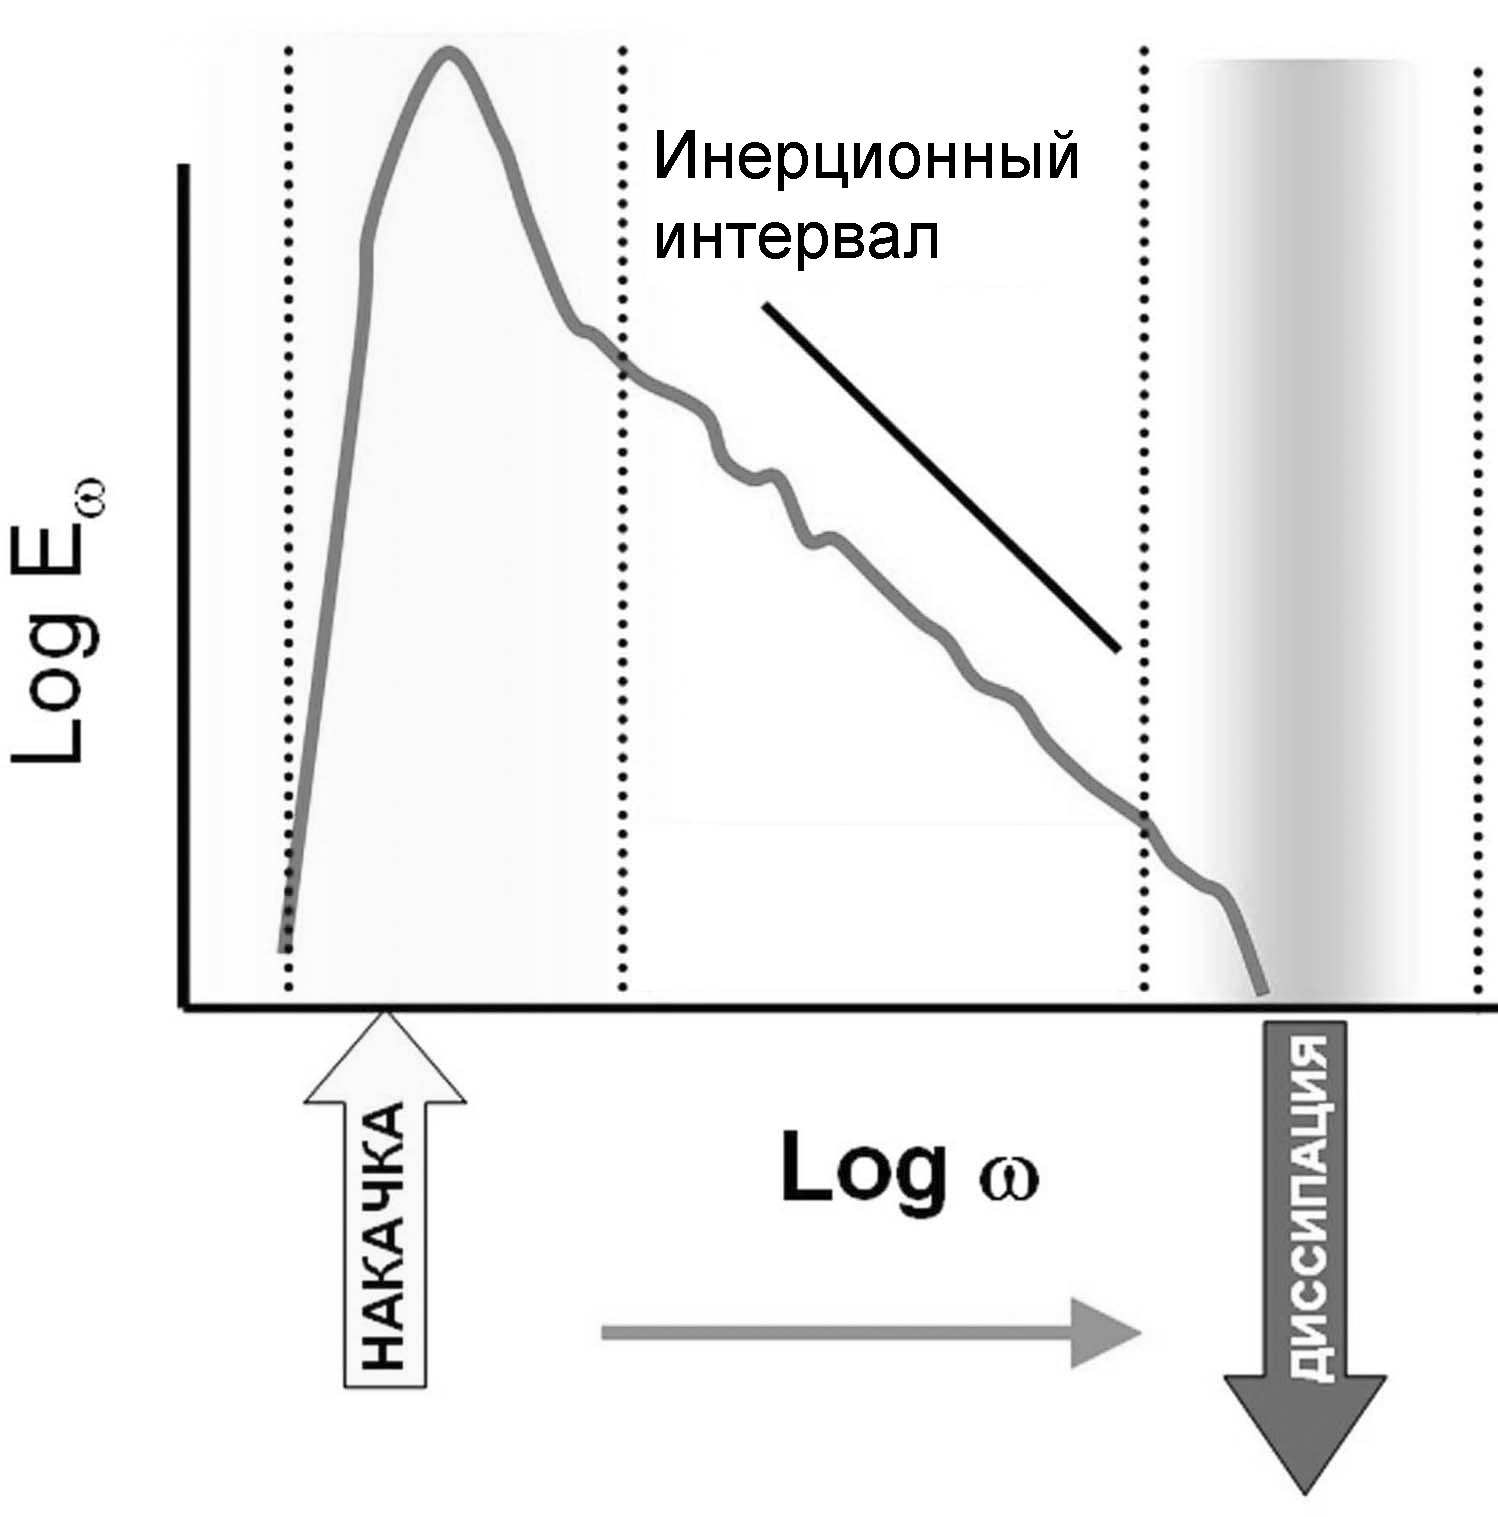
\includegraphics [scale=0.2] {Intro/iner_inter.jpg}
 \caption{} 
 \label{img:turb} 
\end{figure}

Наиболее наглядно волновая турбулентность проявляется в системе волн на поверхности океанов и морей.

Ветер, дующий вдоль изначально гладкой поверхности воды, осуществляет накачку энергии в систему волн из-за неустойчивости Кельвина-Гельмгольца \cite[c. 99]{NonLinearWaves}. При этом масштаб накачки составляет порядка одного сантиметра - капиллярная длина. В результате нелинейного взаимодействия образуются волны других масштабов, которые также эффективно поглощают энергию ветра - ветровые волны, и энергия передается как в сторону коротких волн, так и в сторону длинных волн. В результате нелинейных процессов на поверхности воды могут образоваться большие волны с характерной длиной волны в сотни метров и даже километры. 

Обратим внимание, что в стационарном турбулентном каскаде в системе волн осуществляется баланс энергии: сколько энергии приходит в систему, столько же и диссипирует в результате вязкого трения на малых масштабах, где вязкое затухание является доминирующим механизмом. Т.е. прямой каскад в волновой системе обеспечивает диссипацию энергии приходящей от внешнего источника. 


\section{Закон дисперсии волн на поверхности жидкости}% \label{subsect1_disper}

Волны на поверхности жидкости формируются за счет силы гравитации и сил поверхностного натяжения, причем для длинных волн преобладает влияние гравитации, а для коротких волн определяющими являются капиллярные силы. Это хорошо видно из закона дисперсии для поверхностных волн, однозначно связывающего угловую частоту волны $\omega$ и модуль волнового вектора $\mathbf{k}$ волн на свободной поверхности жидкости:
\begin{equation}
 \label{eq:disper_dip}
\omega^2 = (gk + \sigma/\rho k^3)th(kh),
\end{equation}
где $g$ - ускорение свободного падения, $\sigma$ - коэффициент поверхностного натяжения, $\rho$ - плотность жидкости, $h$ - глубина жидкости.

В случае, когда $k \gg (g\rho/\sigma)^{1/2}$ влияние гравитационных сил становится пренебрежимо малым по сравнению с капиллярными силами. Такие волны называют капиллярными. Волновые вектора $k \ll (g\rho/\sigma)^{1/2}$ соответствуют гравитационному участку закона дисперсии. В промежуточном случае, когда $k \sim (g\rho/\sigma)^{1/2}$, говорят о капиллярно-гравитационных волнах. Для свободной поверхности воды характерная частота перехода от гравитационных волн к капиллярным составляет $\sim$ 17 Гц, при этом длина волны равна $\lambda = 2\pi/k \approx$ 1.5 см. Для поверхности жидкого водорода эта частота также равняется $\sim$ 17 Гц, и ей соответствует длина волны $\approx$ 1.1 см.


Так как плотность жидкого водорода в 13 раз меньше плотности воды, то для возбуждения волн одинаковой амплитуды на поверхности жидкого водорода требуются значительно меньшие силы, чем для генерации волн на поверхности воды. В объем жидкого водорода можно ввести заряды различными методами. При приложении электрического поля перпендикулярно поверхности она заряжается. Затем, если в дополнение к постоянному поля добавить переменное, то можно возбуждать волны, воздействую электрическим полем непосредственно на заряженную поверхность. Это приводят к уникальной возможности экспериментального изучения слабой волновой турбулентности \cite{Kolmakov2006}. Использование жидкого водорода в экспериментах по волновой турбулентности способствовало наблюдению явлений предсказанных волновой теорией, например стационарный спектр Захарова-Колмогорова в капиллярной турбулентности в широком диапазоне частот \cite{Brazhnikov2001}, а также позволило наблюдать новые явления, которые были успешно объяснены в рамках приближения теории слабой волновой турбулентности: например квазиадиабатический распад капиллярной турбулентности \cite{quasiadiabatic} и подавление высокочастотных турбулентных колебаний добавлением низкочастотной возбуждающей силы \cite{addLowFreq}.

Стоит отметить, что если глубина жидкости больше, чем характерная длина волны, то $kh\gg 1$ и $th(kh)$ можно считать равным 1. Таким образом, в приближении глубокой воды дисперсия гравитационно-капиллярных волн записывается как:


\begin{equation}
 \label{eq:disper}
\omega^2 = gk + \sigma/\rho k^3,
\end{equation}


В экспериментах с гравитационными волнами глубина жидкости была около $ h \approx 7$ см, минимальный волной вектор $k \approx 0.36$ см$^{-1}$, соответственно $th(kh) \approx 0.99$, т.е. влиянием глубины можно пренебречь.


В области высоких частот, где можно пренебречь влиянием гравитационных сил, закон дисперсии будет капиллярным:
\begin{equation}
 \label{eq:disperCap}
\omega^2 = \sigma/\rho k^3
\end{equation}



\section{Законы сохранения энергии и импульса} 
При взаимодействии капиллярных волн выполняются законы сохранения энергии и импульса:
\begin{equation}
 \label{eq:saveOmega}
\omega_1 = \omega_2 \pm \omega_3
\end{equation}
\begin{equation}
 \label{eq:saveK}
\mbox{\boldmath$k_1$} = \mbox{\boldmath$k_2$} \pm \mbox{\boldmath$k_3$}
\end{equation}

Отметим, что если в законы дисперсии волн $\omega \sim k ^ \alpha$ показатель степени $\alpha > 1$, то трехволновые процессы распада-слияния волн удовлетворяют законам сохранения импульса и энергии. Такой закон дисперсии называют распадным. Если $\alpha < 1$ , трехволновые процессы запрещены, и основным взаимодействием волн являются четырех волновые процессы. В системе гравитационных волн трехволновые процессы запрещены, и основными являются четырехволновые. 

Таким образом, при возбуждении на поверхности жидкости капиллярных волн может быть сформировано турбулентное состояние, в котором поток энергии направлен из области низких частот(область накачки) в сторону высоких частот. Теория слабой волновой турбулентности \cite{Zakharov} предсказывает, что основной вклад в перенос энергии по турбулентному капиллярному каскаду вносят трехволновые процессы слияния волн - поток энергии направлен в сторону высоких частот. 


\section{Инерционный интервал турбулентного каскада}% \label{subsect1_1_3}

Как было сказано выше характерной особенностью турбулентного каскада является наличие инерционного интервала - частотного диапазона в котором энергия, в основном, передается в k-пространстве из одного масштаба в другой в результате нелинейного взаимодействия волн. 
В настоящий момент имеется довольно много теоретических и экспериментальных работ посвященных изучению распределения энергии в инерционном интервале турбулентного каскада в различных системах. Теория слабой волновой турбулентности предсказывает степенное распределение энергии по шкале частот \cite{Zakharov}:
\begin{equation}
\label{eq:EOmega}
E_\omega \sim \omega^{-\alpha}
\end{equation}

С экспериментальной точки зрения удобно исследовать не распределение энергии по волновым векторам(или частотам), а парную корреляционную функцию отклонения поверхности от положения равновесия $I(\tau)=<\eta(r, t+\tau)\eta(r,t)>$, так как величину отклонения поверхности от положения равновесия, в отличии от энергии, можно непосредственно измерить в эксперименте. Фурье образ парной корреляционной функции отклонения поверхности от равновесного состояния связан с распределением энергии по частотам формулой:
\begin{equation}
\label{eq:EOmegaI}
I_\omega \sim E_\omega \omega^{-4/3} = n(\omega) \omega^{-1/3},
\end{equation}
где $n(\omega)$ - функция распределения капиллярных волн.

Таким образом предсказывается степенная зависимость парной корреляционной функции от частоты $I_\omega \sim \omega^{-m}$ в инерционном интервале.

В зависимости от характера накачки теория волновой турбулентности предсказывает различные значения показатели $m$. Для широкополосной накачки (когда ширина полосы накачки сопоставима с частотой накачки), предсказывается $m$ = 17/6. При накачке узкополосным сигналом в спектре появляются равноудаленные пики, максимумы которых убывают c ростом частоты с показателем $m$ = 23/6. Данные предсказания подтверждаются как компьютерным моделированием \cite{Babiano1995, Babiano1987, Falcovich1988, Pushkarev1996}, так и экспериментальными исследованиями распределения $I_\omega$
в спектрах турбулентных каскадов в системе волн на поверхности воды \cite{BrazhnikovWater}, жидкого водорода \cite{Brazhnikov2001}, жидкого гелия \cite{Abdurakhimov2007}, ртути \cite{Falcon2007}.

Стоит отметить, что одной из сложностей экспериментального исследования турбулентных каскадов является степенное уменьшения энергии волны с ростом частоты. Так как величина показателя степени $m$ находится в районе 2-3, а диапазон частот, в котором существует турбулентный каскад, может достигать нескольких декад, то для экспериментального исследования поведения турбулентной системы в достаточно широком диапазоне частот, необходимым условием для наблюдения развитого турбулентного каскада, является наличие экспериментального оборудования обладающего большим динамическим диапазоном. По этой причине экспериментальные исследования были практически невозможны до появления широко распространенных АЦП с высоким динамическим диапазоном и достаточно высокой частотой оцифровки, а также компьютерной техники и программного обеспечения для обработки полученных сигналов.

\section{Положение высокочастотной границы инерционного интервала}\label{subsect_hiFreqBound}

При определении частотной области, где заканчивается инерционный интервал и начинается диссипация энергии важную роль играют такие характеристики волновой системы как время вязкого затухния волны и время нелинейного взаимодействия волн.

Время вязкого затухания волны на частоте $\omega$ \cite[стр. 135]{land}.
\begin{equation}
\label{eq:tauNu}
1/\tau_\nu = 2\nu k^2 = 2 \nu \omega^{4/3}(\sigma/\rho)^{2/3},
\end{equation}
где $\nu$ - кинематическая вязкость жидкости.
То есть вязкое время уменьшается с ростом частоты, а следовательно и диссипация энергии на более высоких частотах сильнее.


Характерное время нелинейного взаимодействия капиллярных волн можно выразить через параметры жидкости и функцию распределения капиллярных волн $n(\omega)$:
\begin{equation}
\label{eq:tauNl}
1/\tau_{nl} = |V_\omega|^2 n(\omega)
\end{equation}

Где $V(\omega) \approx (\sigma/\rho^{3/2})\omega^{3/2}$ - коэффициент трехволнового нелинейного взаимодействия капиллярных волн.

%Функцию распределения капиллярных волн $n(\omega) \sim E_{\omega}\omega^{-1}$ 
В развитом турбулентном каскаде энергия передается от низких частот к высоким практически без потерь до тех пор, пока поток энергии волн, переходящий в тепло, не становится сравнимым с потоком энергии по каскаду. Таким образом, положение высокочастотной границы инерционного интервала можно определить как частоту, на которой совпадают времена вязкого затухания и нелинейного взаимодействия волн.

Из уравнений (\ref{eq:EOmegaI}, \ref{eq:tauNu}, \ref{eq:tauNl}), используя известные значения $m$ = 17/6 для широкополосной накачки и $m$ = 23/6 для монохроматической накачки, получаем оценку амплитудной зависимости частоты границы инерционного интервала $\omega_b \sim \eta_p^{12/5}$ для широкополосной накачки и $\omega_b \sim \eta_p^{4/3}$ для узкополосной накачки. Отметим работу \cite{Brazhnikov_bound_freq}, в которой изучалось поведения положения границы инерционного интервала при вариациях частоты и амплитуды монохроматической накачки в цилиндрической геометрии. Работы направленные на понимание общей картины поведения положения границы инерционного интервала при различных типах накачки в экспериментальных ячейках разной геометрии в литературе не встречались.
%хренности $\Omega_0$ в случае стоячих волн определяется как:

\section{Диссипативная область турбулентного каскада}% \label{subsect_disp}

На высоких частотах, выше границы инерционного интервала, распределение $I_\omega$ определяется спектральной характеристикой накачки, нелинейным взаимодействием и затуханием волн. В диссипативной области время вязкого затухания волн не превышает время нелинейного взаимодействия: преобладают процессы затухания. Однако нелинейные процессы существенно влияют на форму спектра. Если волны в диссипативном интервале взаимодействуют в основном с ближайшими соседями, а не с волнами из инерционного интервала, то распределение энергии по волнам в области диссипации становиться близким к экспоненциальному.
Если же волны в диссипативной области $\omega \gg \omega_b$ взаимодействует волнами из инерционного интервала $\omega \ll \omega_b$, то распределение энергии по волнам несколько отличается от экспоненциального. Детальное рассмотрение дает “квазипланковский” спектр корреляционной функции в диссипативной области \cite{Ryzhenkova1990}
\begin{equation}
% \label{eq:tauNu}
<\eta_\omega^2> \sim \omega^{-s} e^{-\omega/\omega_d},
\end{equation}			
где s - некая константа. Численные вычисления для дискретного кинетического уравнения \cite{Ryzhenkova1990} подтверждают экспоненциальную зависимость волнового числа заполнения в области сильного затухания. Величину $\omega_d$ имеющую размерность частоты и отвечающей за то насколько быстро затухает турбулентный спектр в диссипативной области будем называть частотой вязкого затухания спектра в диссипативной области.
	
Экспериментальные ячейки имеют конечные размеры, поэтому спектр поверхностных возбуждений носит дискретный характер. Это накладывает дополнительные ограничения на выполнение законов сохранения энергии и импульса \cite{Kartashova1991}. В экспериментальных работах \cite{Brazhnikov2014, Aburakhimov2015} было показано, что выбором размеров ячейки при накачке на фиксированных частотах можно организовать передачу энергии как на высокие, так и на низкие частоты.
Одной из целей настоящей работы было проведение подробных исследований зависимостей высокочастотного края инерционного интервала $\omega_b$ и характерной частоты $\omega_d$ от амплитуды возбуждающей силы на поверхности воды в цилиндрической и квадратной ячейках при амплитудах накачки меньше порогового значения, при котором возникает параметрическая неустойчивость Фарадея.

\section{Дискретные моды колебаний поверхности жидкости в ячейке конечных размеров} %\label{subsect1_geometr}

Распределение волн на поверхности жидкости сильно зависит от геометрии сосуда и от способа возбуждения их возбуждения.
В случае, если затухание волн мало, при их возбуждении на поверхности жидкости возникнет система стоячих волн. Форма стоячих волн будет зависеть от граничных условий и возбуждаемой моды. Граничным условием для волн в ячейке конечных размеров является неспособность воды проходить через стенку ячейки, т.е. нормальная (к стенке ячейки) компонента скорости жидкости должна быть равна нулю. Для цилиндрической ячейки радиуса $r_0$ резонансные моды волн будут описываться функцией Бесселя:

\begin{equation}
 \label{eq:Bessel}
h(r, \phi, t) = A J_0(k_nr) cos(m\phi) cos(\omega t),
\end{equation}
причем $k_n$ должна удовлетворять требованию ${J_0}'(k_nr_0) = 0$. Иными словами на границе ячейки должна быть пучность стоячей волны.

Если $m$ = 0, то мода будет радиальной, в таком случае скаляр $k$ играет роль волнового числа: при больших значениях $R/\lambda$, ($\lambda = 2\pi/k$ – длина возбуждаемой волны) и на большом расстоянии $r \gg \lambda$ от центра ячейки в узком угловом секторе цилиндрическую волну можно рассматривать как плоскую волну с волновым числом $k$ в одномерном k-пространстве.

В прямоугольной ячейке стоячие волны описываются суммой двух стоячих перпендикулярных синусоидальных волн:
\begin{equation}
\label{eq:waveStand}
h(x, y, t) = A_1 sin(kx)cos(\omega t)+A_2 sin(ky)cos(\omega t+ \phi)
\end{equation}
где $\phi$ разность фаз между стоячими волнами в разных направлениях.

Бегущие волны, распространяющиеся от двух перпендикулярных стенок прямоугольной ячейки будут задаваться выражением:
\begin{equation}
\label{eq:waveRun}
h(x, y, t) = A_1 sin(kx-\omega t)+A_2 sin(ky-\omega t+ \phi)
\end{equation}



\section{Возбуждение волн в ячейке, совершающей колебания в вертикальном направлении} \label{p1_methodsExt}
Турбулентноcть на поверхности воды в гравитационно-капиллярном интервале частот изучалась многими исследователями в течение нескольких последних десятилетий \cite{Falcon2007, Henry2000, Shats2010, Denissenko2007}. Для возбуждения волн использовали различные методики. В лабораторных условиях волны на поверхности жидкости могут возбуждаться различными способами: при помощи волнопродукторов \cite{Havelock1929, Falcon2007}, электрическими силами, действующими на границу раздела жидкостей с разной диэлектрической проницаемостью \cite{Kalinichenko1982} или на поверхность заряженной жидкости \cite{Brazhnikov2002}. Однако в большинстве работ для генерации волн используют параметрическую неустойчивость поверхности жидкости, совершающей вынужденные вертикальные колебания с ускорениями выше некоторого порогового значения (неустойчивость Фарадея) \cite{Henry2000, Shats2010, Denissenko2007}. Отличительной чертой этой методики является высокий уровень возбуждения волн сразу после возникновения неустойчивости на поверхности. Такая особенность методики возбуждения не позволяет работать с волнами малой амплитуды. Кроме того, как выяснилось, при сильном возбуждении наряду с нелинейным взаимодействием волн наблюдается генерация вихревого движения \cite{VonKameke2011, Francois2013}. Недавно в \cite{F5, F6} было показано, что завихренность формируется в результате взаимодействия нелинейных волн, имеющих неколлинеарные волновые векторы $\mathbf{k}$. В \cite{BrazhnikovWater} волны на поверхности цилиндрической ячейки возбуждали с помощью кольца, касающегося поверхности воды вблизи стенок ячейки. На поверхности возбуждалась только радиальная мода. В этом случае стоячие волны на поверхности описываются функцией Бесселя параметра $Rk$ ($R$ – радиус ячейки). Экспериментальные результаты \cite{BrazhnikovWater} оказались в хорошем согласии с теорией слабой (волновой) турбулентности \cite{Zakharov}.


При вертикальных колебаниях ячейки возможны два механизма возбуждения волн на поверхности воды. Первый осуществляется благодаря наличию мениска на границе ячейки. При вертикальных колебаниях равновесный радиус мениска меняется в зависимости от величины вертикального ускорения, что приводит к появлению на поверхности жидкости волн с частотой равной частоте вертикальных колебаний ячейки. 

Второй механизм возникновения волн обусловлен развитием параметрической неустойчивости на поверхности жидкости, впервые описанной Фарадеем \cite{Faraday1831}. Неустойчивость Фараде является параметрической, а частота возбуждаемой волны оказывается в два раза меньше частоты вертикальных колебаний ячейки. 

При вертикальных колебаниях сосуда с относительно низкой амплитудой параметрическая неустойчивость Фарадея не возникает, так как неустойчивость развивается при амплитудах выше некоторого порогового значения. Поэтому для наблюдения спектров турбулентного каскада на поверхности воды использовалось возбуждение волн с помощью вертикальных колебаний с амплитудой ниже порога параметрической неустойчивости. 

Стоит отметить, что при возбуждении волн на поверхности воды с помощью мениска в цилиндрической ячейки возбуждаются только радиальные моды, а при развитии параметрической неустойчивости происходит возбуждение и азимутальной моды.



При наблюдении волновой турбулентности на поверхности жидкого водорода удобнее использовать возбуждение волн с помощью электрического поля. В этом случае амплитуда волн ограничивается напряжением пробоя и размерами оптического окна криостата, через которое с помощью лазерного луча производится регистрация волн \cite{Brazhnikov2002}.


\section{Метод детектирования волн на поверхности жидкости}\label{p1_methodDetect}

Существует несколько методик регистрации капиллярных волн. Можно регистрировать волны на поверхности жидкости с помощью преломленного или отраженного лазерного луча от сравнительно небольшого участка поверхности жидкости \cite{Brazhnikov_IET}. Для регистрации волн на поверхности проводящей жидкости в работе \cite{Falcon2007} в жидкость вводили вертикально ориентированный отрезок изолированной металлической проволоки. В результате образуется цилиндрический конденсатор, одной из обкладок которого служит поверхность проволоки, а другой – проводящая жидкость. По изменению емкости конденсатора со временем можно судить о колебаниях уровня жидкости в точке контакта изолированной проволоки и жидкости.
В работе \cite{Wright1996, Henry2000} камерой регистрировали свет прошедший через полупрозрачную жидкость, а для обеспечения диффузного распространения света в объеме жидкости в рабочую ячейку с жидкостью (водой) вводили полистироловые шарики диаметром 1 мкм или добавляли обычное молоко. На фотографии колеблющейся поверхности яркость отдельных точек определяется высотой уровня поверхности жидкости, т.е. по распределению яркости точек на поверхности можно судить о распределении энергии (амплитуде колебаний) по волновым векторам на поверхности освещаемой снизу "мутной" жидкости. В работе \cite{Fujimura2008} возбуждение и регистрация колебаний на поверхности воды производится с помощью электрического поля емкостным методом. Для этого на стенке прямоугольной кварцевой кюветы помещены полоски из алюминия, которые играют роль конденсатора.

Остановимся подробнее на методики регистрации волн с помощью отраженного лазерного луча.

\begin{figure}[ht] 
 \center
 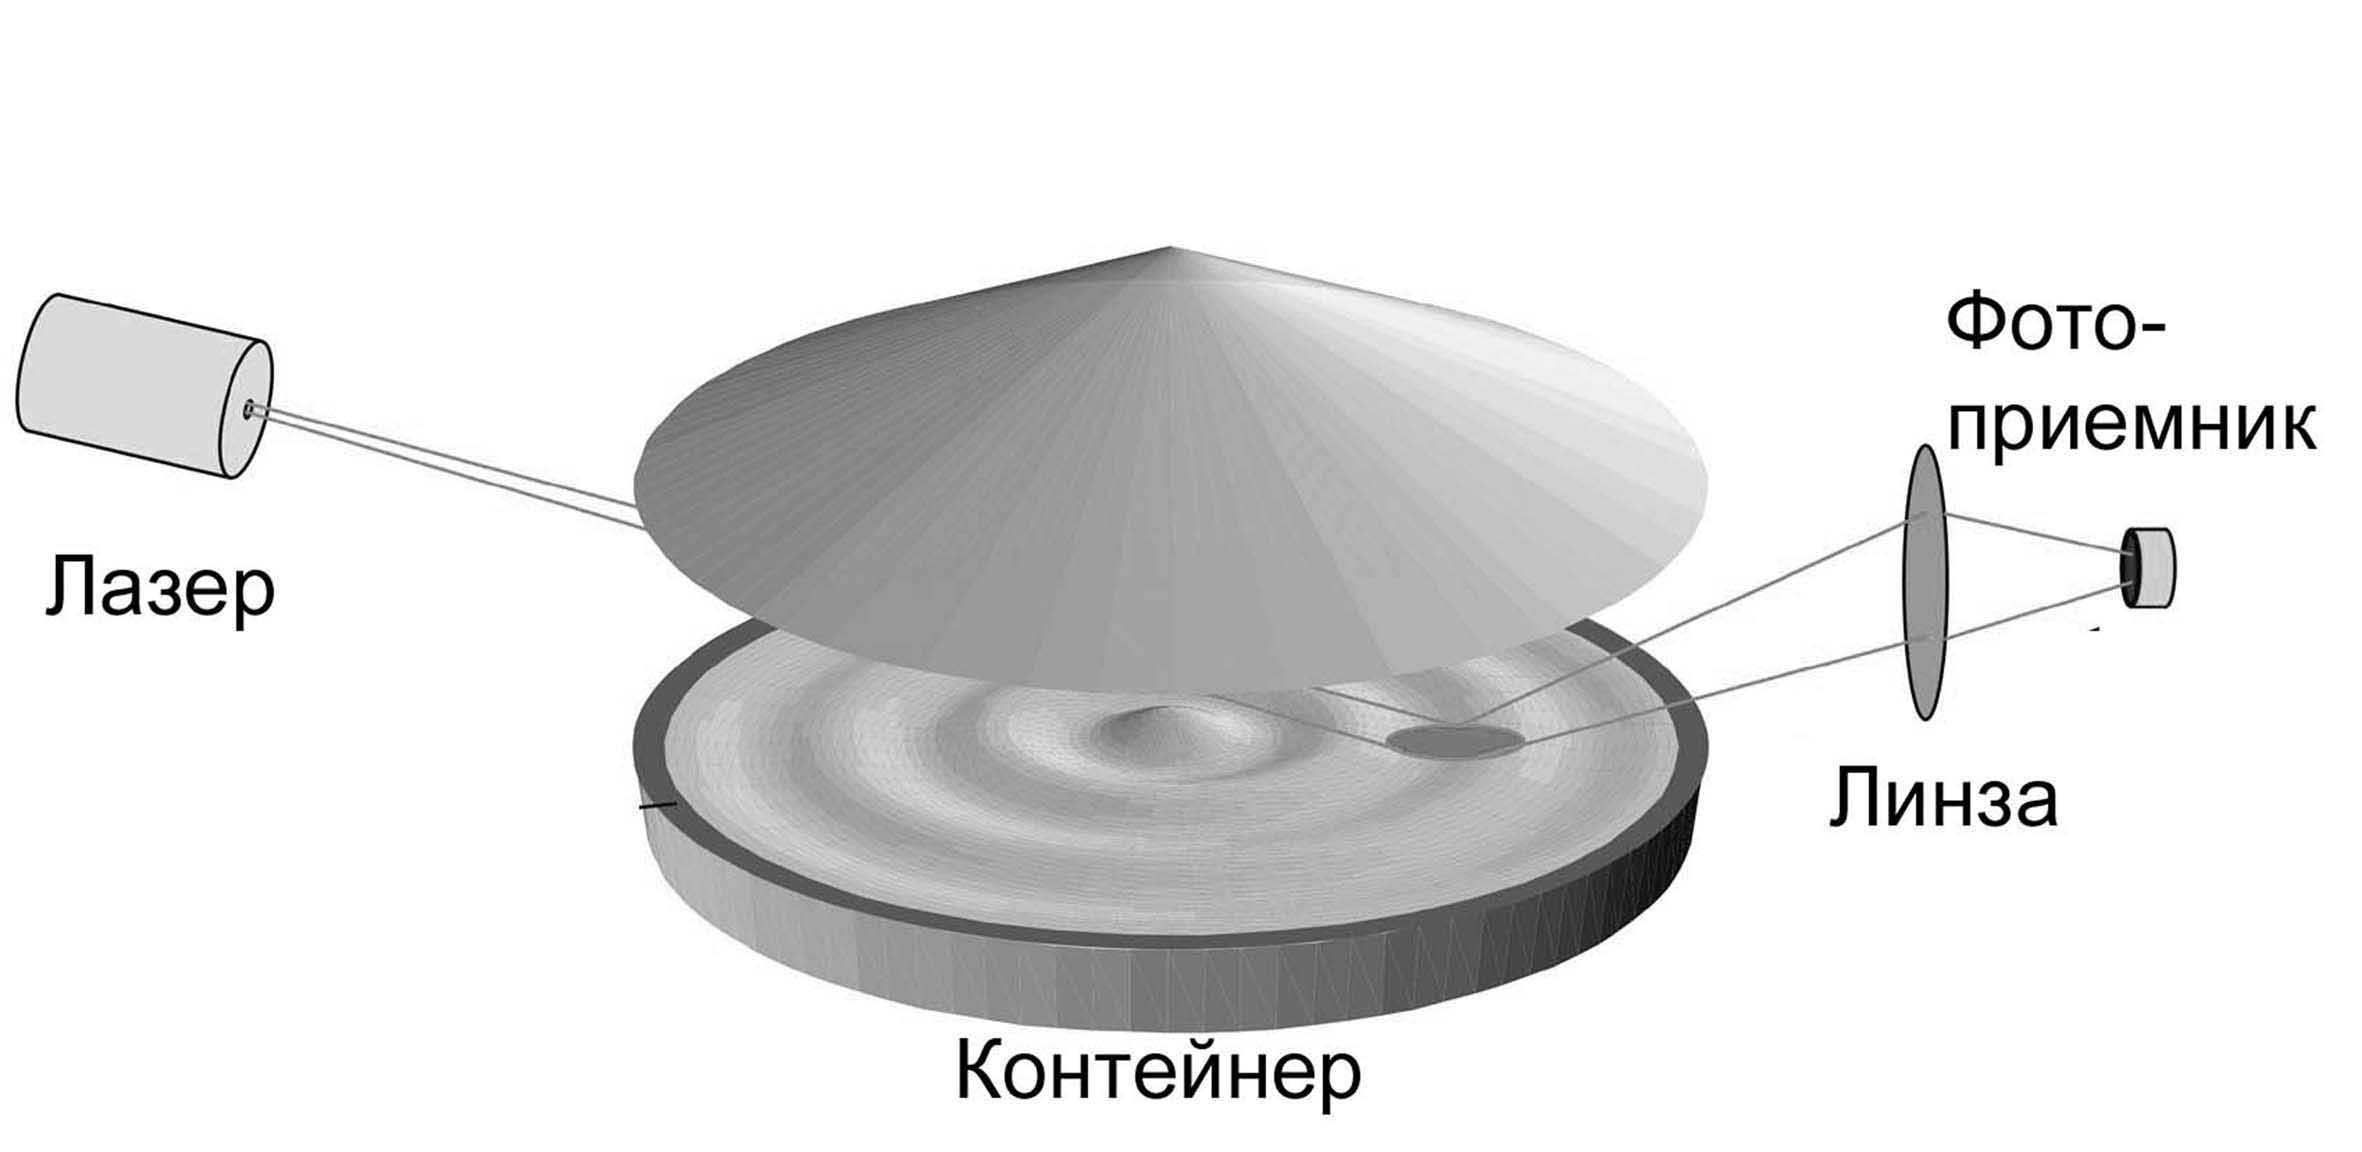
\includegraphics [scale=0.15] {Intro/laser.jpg}
 \caption{Схема методики измерения волн на поверхности жидкости с помощью отраженного лазерного луча.} 
 \label{img:laser}
\end{figure}

Колебания поверхности детектируются по схеме, показанной на рисунке \ref{img:laser}. Лазерный луч, отраженный от поверхности жидкости, фокусируется линзой на фотоприемник. Угол скольжения лазерного луча (угол между лазерным лучом и плоскостью поверхности жидкости) к поверхности жидкости составляет примерно 0.2 рад. Максимальный угол отклонения поверхности жидкости от равновесия составляет 0.05 рад.

В зависимости от характерного размера $a$ пятна лазерного луча на поверхности жидкости и длины волны $\lambda$ детектируемого колебания возможны два метода обработки сигнала с фотоприемника:

1. $ a \ll \lambda$. "Узкий луч". Характерный размер пятна лазерного луча много меньше длины волны. В этом случае мощность отраженного луча зависит от угла отражения, то есть в приближении малых углов мощность принимаемого сигнала фотоприемника линейно зависит от угла отражения.
\begin{equation}
%\label{eq:waveStand}
P(t) \sim R(\alpha + \phi(t)) \approx R(\alpha) + const \phi(t)
\end{equation}
Для квадрата Фурье-компонент:
\begin{equation}
%\label{eq:waveStand}
P^2_\omega \sim \phi^2_\omega
\end{equation}
где $P(t)$ - мощность сигнала на фотоприемнике, $R$ – коэффициент отражения.

2. $a \gg \lambda$. "Широкий луч". Характерный размер пятна лазерного луча много больше длины волны. В этом случае мощность отраженного луча является интегральной характеристикой поверхности. В результате усреднения получится следующая зависимость \cite{Brazhnikov_IET}:
\begin{equation}
%\label{eq:waveStand}
P^2_\omega \sim I_\omega
\end{equation}

\section{Возбуждение вихревых течений поверхностными волнами}% \label{sect3_1}

Сравнительно недавно было обнаружено, что при параметрическом возбуждении наряду с волновым движением на поверхности жидкости также наблюдается течение, демонстрирующее хаотическое поведение \cite{Ramshankar1990}. Впоследствии было показано, что это течение соленоидально и с увеличением амплитуды волн может оказаться достаточно интенсивным для формирования турбулентного каскада \cite{VonKameke2011, Francois2014, Francois2013} подобно обратному каскаду в двумерной турбулентности \cite{Kraichnan1967}. Несмотря на большое количество экспериментальных исследований, посвященных волнам Фарадея, природа возникновения в них течения до настоящего времени не была выяснена. В работе \cite{Mesquita1992} это течение пытались описать как средний дрейф Стокса \cite{Stokes1847} для случайного волнового поля. Однако найденное в эксперименте значение коэффициента диффузии пассивного скаляра почти на порядок превышало теоретическое.	
	Наше исследование показало \cite{F5}, что генерация вихревого движения не является особенностью неустойчивости Фарадея, а является следствием нелинейного взаимодействия волн, распространяющихся под углом друг к другу. Таким образом данное явление уже имеет отношение к движению поверхности океана. В частности оно может играть значительную роль в перемешивании планктона и в движении загрязняющих веществ на поверхности воды \cite{Falkovich2009}.
	Стоит еще отметить, что изучив механизм генерации вихревых течений поверхностными волнами можно научиться создавать вихревое движение заданное формы, возбуждая на поверхности волны силой с рассчитанной спектральной характеристикой.
	
Для количественного изучения вихревых движений используется величина завихренности, определяемая как:

\begin{equation}
 \label{eq:defVort}
\Omega(x, y) = \frac{\partial V_x}{\partial y} - \frac{\partial V_y}{\partial x}
\end{equation}
где $V_x$, $V_y$ – компоненты скорости жидкости. 

\section{Дрейф Стокса} \label{p1_Stockes}

Волновое движение на свободной поверхности жидкости описывается гармоническим колебанием, затухающим в глубину \cite{land}:

\begin{equation}
 \label{eq:waveSimple}
 V_x(x,z,t) = -A k e^{kz}sin(kx-\omega t)
\end{equation}

\begin{equation}
 V_z(x,z,t) = A k e^{kz}cos(kx-\omega t)
\end{equation}

Несмотря на то, что среднее по периоду колебаний значение скорости в любой точке пространства равно 0, пробная частичка, помещенная в жидкость будет иметь не нулевое смещение за период колебания. Это связано с тем, что поле скорости жидкости меняется со временем, и для подсчета величины смещения пробной частички в пространстве необходимо интегрировать скорость жидкости по траектории движения пробной частички. В результате изменения скорости жидкости со временем траектория пробной частички получается незамкнутой и смещающейся за каждый период, см. рис. \ref{img:stockesTrack}.

\begin{figure}[ht] 
 \center
 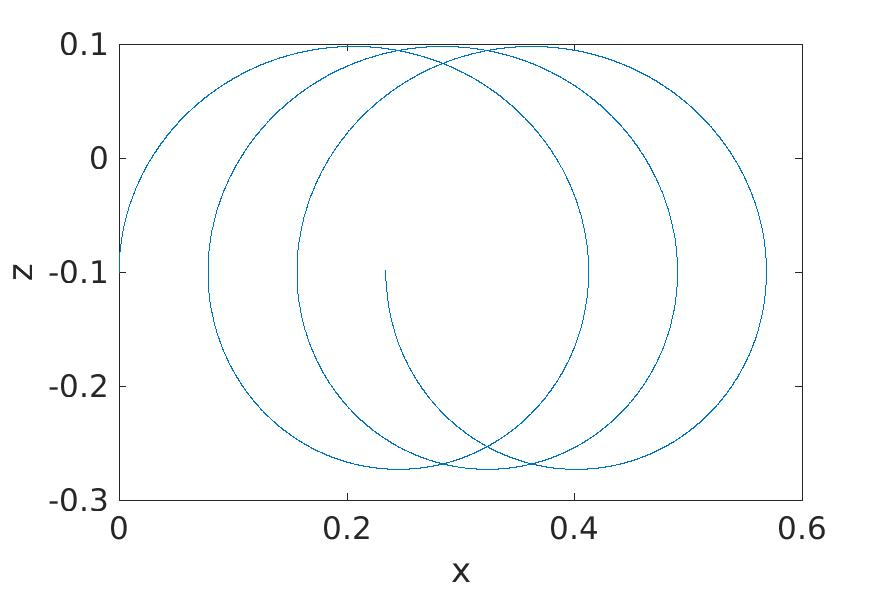
\includegraphics [scale=0.2] {Intro/StockesTrack.jpg}
 \caption{} 
 \label{img:stockesTrack} 
\end{figure}

Другими словами пробная частичка в волне будет совершать колебания, смещаясь в сторону распространения волны. Среднюю скорость смещения можно оценить как \cite{FalkovichBook}:
\begin{equation}
 \label{eq:StockesVel}
	V_{St} = A^2 k^3 /2 \omega
\end{equation}

Бегущая волна создает перенос массы с направлении своего распространения, который прекращается сразу же, когда прекращается волновое движение в данной точке пространства.

Представление уравнений движения жидкости, когда в качестве скоростей жидкости используется скорости жидкости в определенных точках пространства - называется эйлеровым. В лагранжевом представлении исследуется скорости определенных объемов жидкости. При движении бегущей волны средняя эйлерова скорости будет равна нулю, в то время как средняя лагранжева скорость будет равна дрейфу Стокса.

При регистрации движения декорирующих частиц на поверхности жидкости может регистрироваться как лагранжева скорость, так и эйлерова. Для регистрации эйлеровой скорости необходимо выполнение следующих условий: частота съемки должна быть много больше частоты волны и шаг пространственной сетки регистрации должен быть много меньше амплитуды колебания кусочка жидкости за период волны. Так как второе условие в наших экспериментах технически выполнить сложно, то стоит считать, что в наших экспериментах измеряется лагранжева скорость.


%\clearpage           % Введение
\chapter{"Квазипланковский" спектр капиллярной турбулентности на поверхности жидкого водорода}


В турбулентном каскаде область накачки и диссипации значительно разнесены в пространстве волновых векторов. Наличие диссипативной области является необходимым условием для установления турбулентного каскада. В диссипативной области турбулентного распределения механическая энергия волн переходит в тепло в результате вязких потерь. Энергия в диссипативную область поступает в результате нелинейного взаимодействия волн с гармониками из инерциального интервала. Распределение энергии в диссипативной области определяется характером волнового взаимодействия как внутри области, так и с волнами более низкой частоты \cite{Ryzhenkova1990}. 
В этой главе представлены результаты исследования распределения энергии по частоте в диссипативной области турбулентного каскада в системе капиллярных волн на поверхности жидкого водорода. При изучении волновой турбулентности жидкий водород выгодно отличается от воды в пять раз более низким коэффициентом кинематической вязкости и в три раза большим коэффициентом нелинейности капиллярных волн, который оценивается как $V \sim (\sigma / \rho^3)^{1/4}$ . Таким образом, при равных угловых амплитудах волн на частоте накачки относительная ширина инерционного интервала, оцениваемая из равенства времен вязкого затухания волн, оказывается в три раза больше для водорода. 

\section{Экспериментальная методика} %\label{sect1_1}
 Экспериментальная установка состоит из гелиевого криостата, в вакуумной полости которого расположена оптическая ячейка, системы возбуждения колебаний на поверхности жидкости и оптической системы их. Цилиндрический стакан изготовленный из меди 6 мм глубиной и 60 мм внутренним диаметром был установлен внутри ячейки. На расстоянии 4 мм над стаканом располагается металлическая пластина. Газообразный водород сконденсируется в стакан до максимального уровня. Радиоактивная мишень (молибденовая пластина, покрытая слоем тритида титана), расположенная на дне стакана, ионизирует жидкий водород. В присутствии постоянного напряжения около 1 кВ между стаканом и верхней пластиной, положительно заряженные ионы собираются под поверхностью жидкого водорода, образуя квазидвумерный слой. Волны на поверхности жидкого водорода возбуждаются дополнительным к постоянному переменным напряжением с максимальной амплитудой около 100 В. Более подробно эта методика возбуждения волн описана в \cite{Brazhnikov_IET}

\begin{figure}[ht] 
 \center
 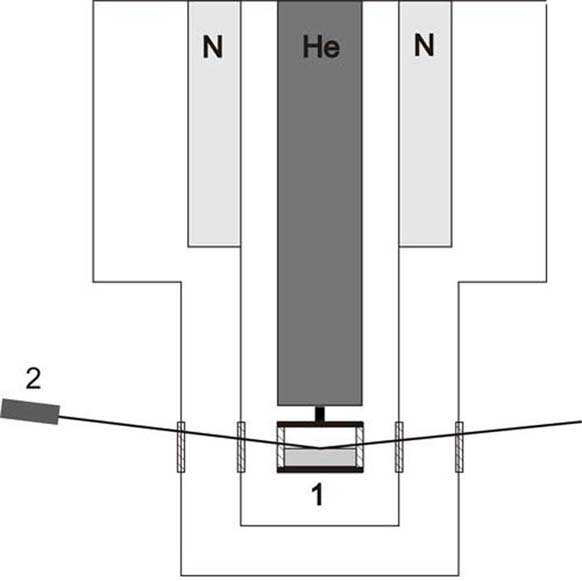
\includegraphics [scale=0.4] {article1/kriostat.jpg}
 \caption{Схематичная конструкция криостата.
 1 – экспериментальная ячейка, 2 – лазер.} 
% \label{img:hydr_specrta_dlog} 
 
\end{figure}


\begin{figure}[ht] 
 \center
 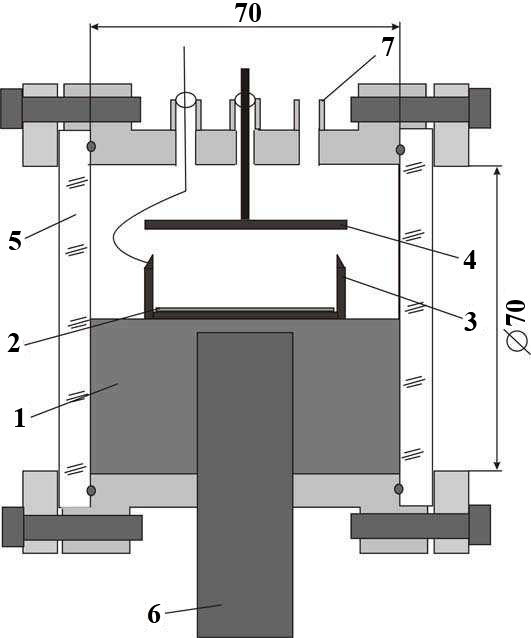
\includegraphics [scale=0.4] {article1/cell.jpg}
 \caption{Схематичная конструкция ячейки. 
 1 – текстолитовый брусок, 2 – радиоактивная мишень, 3 – медный контейнер, 4 – верхняя обкладка конденсатора, 5 – кварцевое окно, 6 - медный хладопровод, 7 – капилляр для набора водорода.} 
% \label{img:hydr_specrta_dlog} 
\end{figure}


	Использование переменного электрического поля позволяет возбуждать на поверхности капиллярные волны хорошо контролируемой силой. В этих экспериментах в качестве переменного возбуждающего напряжения были использованы низкочастотные случайные сигналы. Эти сигналы были синтезированы обратным Фурье-преобразованием случайного набора фаз и прямоугольного амплитудного спектра, который везде равен нулю кроме заданного частотного интервала накачки.
	
\begin{figure}[ht] 
 \center
 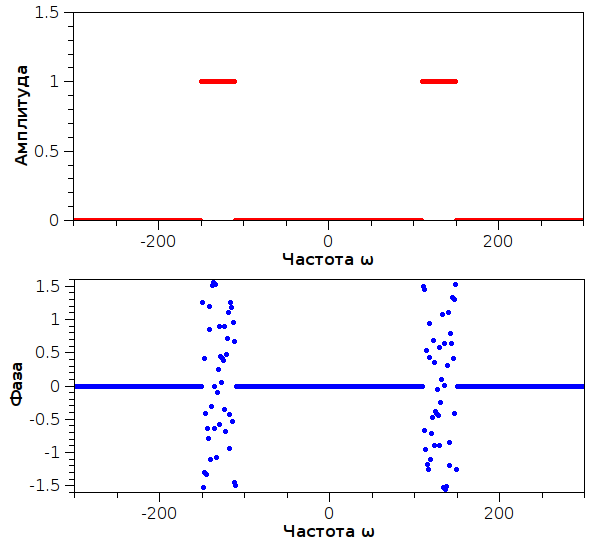
\includegraphics [scale=0.75] {article1/ftt-gen1.png}
 \caption{Частотное распределение амплитуды (верхний график) и пример частотного распределения фазы (нижний рисунок) сигнала, использующегося в качестве накачки.} 
% \label{img:hydr_specrta_dlog} 
\end{figure}
\begin{figure}[ht] 
 \center
 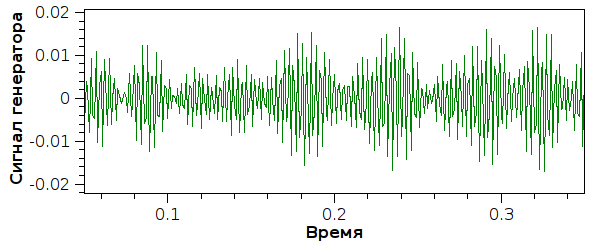
\includegraphics [scale=0.75] {article1/fft-gen2.png}
 \caption{Фрагмент сигнала накачки.} 
% \label{img:hydr_specrta_dlog} 
\end{figure}


	Для регистрации волн на поверхности жидкости использовался метод отражения лазерного луча. Лазерный луч падает под малым скользящим лучом (около 0.2 рад) на поверхность жидкости. Отраженный луч фокусируется линзой на фотодетектор. Напряжение на фотодетекторе усиливается и оцифровывается 24 битным аналогоцифровым преобразователем (ЦАП) с частотой дискретизации около 100 кГц. Волны регистрируются в режиме ''широкого луча'', когда размер лазерного луча больше, чем характерная длина волны. Энергия отраженного лазерного луча $P(t)$ в этом режиме пропорциональна отклонению поверхности $\eta(t)$ \cite{Brazhnikov_bound_freq}. По этой причине в дальнейшем не делается разницы между спектром корреляционной функции отклонения поверхности $<|\eta_\omega^2|>$ и энергии отраженного лазерного луча $<P_\omega^2>$. Более подробно эта методика измерения описана в \cite{Brazhnikov_IET}.

	Максимальная угловая амплитуда волны, которая может быть зарегистрирована в эксперименте, ограничена размером оптических окон криостата и приблизительно равно 0.05 рад.

\section{Экспериментальные результаты и обсуждение} %\label{sect1_1}
 Капиллярные волны возбуждались случайной силой в частотном диапазоне 39-103 Гц. Средний квадрат возбуждающего напряжения менялся от $V_p = 0$ В, т.е. отсутствие накачки, до $V_p = 30$ В, Ограничение связано с максимальной угловой амплитудой волны. На рис. \ref{img:hydr_specrta_dlog} показан пример Фурье-спектра для отраженной энергии лазерного луча $P_\omega^2$ для разных амплитуд возбуждающей силы. На рис \ref{img:hydr_specrta_dlog} хорошо видно область накачки на низкочастотной части спектра. За областью накачки следует инерционный интервал - относительно широкая частотная область, где видна степенная зависимость спектра $P_\omega^2$. Ширина инерционного интервала зависит от амплитуды накачки. Когда поверхность возбуждается слабо (переменное напряжение $V_p = 4$ В) область диссипация начинается рядом с областью накачки и инерционный интервал не наблюдается. Увеличение силы накачки приводит к уширению инерционного интервала, высокочастотная граница инерционного интервала $\omega_b$ смещается к высоким частотам. Наиболее широкий инерционный интервал с границами от $\approx 0.3$ кГц, до $\omega_b \approx 4$ кГц наблюдается при максимальном напряжении накачки $V_p = 30$ В. На частотах выше высокочастотной границы инерционного интервала колебания поверхности затухают из-за вязких потерь, кривая $P_\omega^2$ идет вниз гладко и уходит ниже уровень аппаратных шумов.
 
 \begin{figure}[ht] 
 \center
 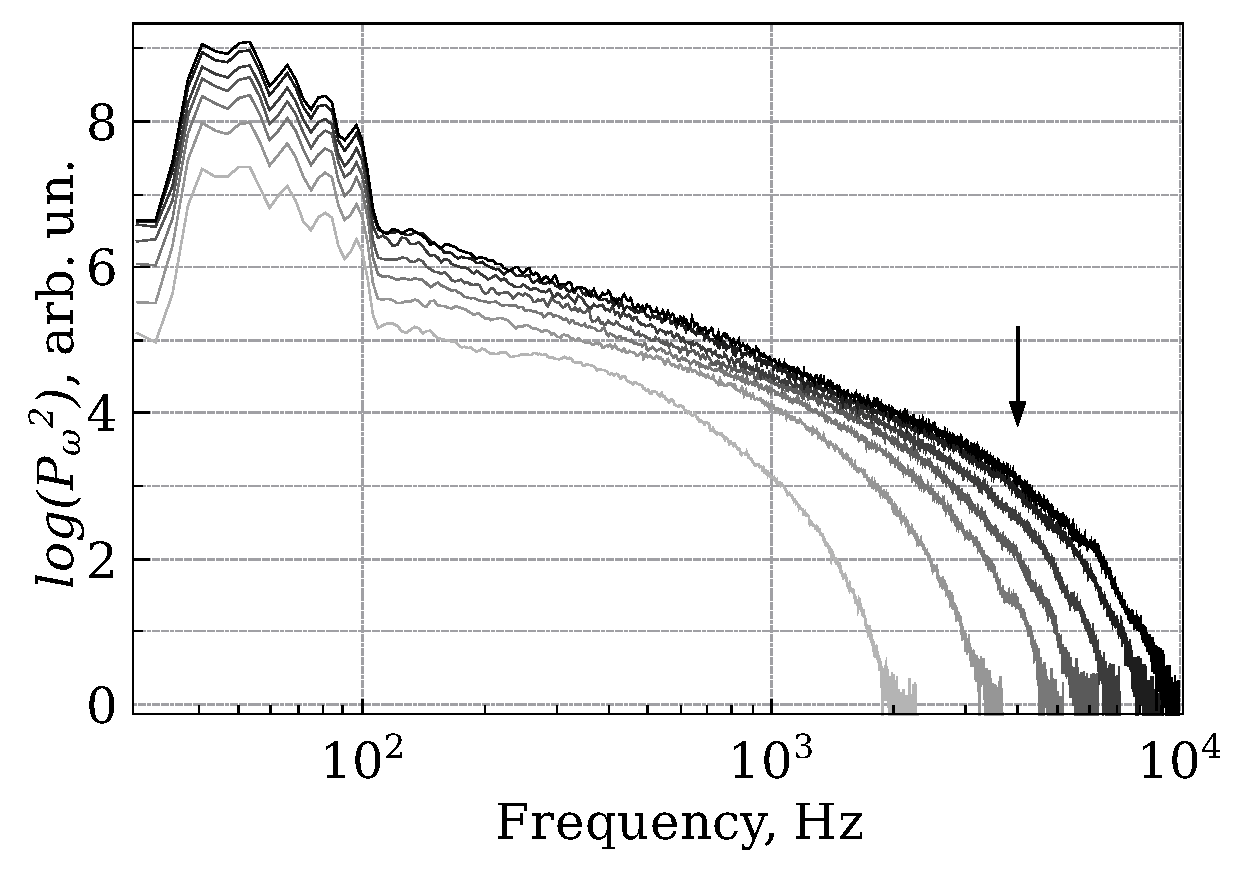
\includegraphics [scale=.8] {article1/spectra_dlog.eps}
 \caption{Спектры поверхностных колебаний $P^2_\omega$ возбужденных случайной силой в частотном диапазоне 39-103 Гц на разных амплитудах возбуждающей силы. Среднеквадратичное значение возбуждающего напряжения $V_P$ меняется от 4 до 30 В. Более темные линии соответствуют большей силе накачки. Стрелкой показана высокочастотная граница инерционного интервала $\omega_b \approx 4$ кГц при накачке 30 В.} 
 \label{img:hydr_specrta_dlog} 
\end{figure}

	Турбулентные спектры, перестроенные в линейном масштабе на рис. \ref{img:hydr_specrta_log} показывают, что убывание амплитуд волн с частотой выше высокочастотной границы инерционного интервала может быть достаточно хорошо описано экспоненциальным затуханием $P_\omega^2 \sim	e^{-\omega/\omega_d}$ в некотором интервале частот. Полученный параметр $\omega_d$ оказывается значительно меньше, чем частоты из интервала подгонки, что разумно для планковского распределения. Например спектр, полученный при амплитуде переменного напряжении накачки $V_p = 26$ В хорошо приближается экспоненциальной функцией в диапазоне 5-9 кГц с $\omega_d \approx 0.6$ кГц. К сожалению, узкий интервал подгонки не позволяет установить показатель степени s "квазипланковского" распределения достаточно точно. Полученные значения $\omega_d$ в несколько раз меньше, чем видимая граница между инерционным интервалом и диссипативной области(см. рис. \ref{img:hydr_specrta_dlog}). Это несоответствие можно отнести к определенной степени свободы в определении граничной частоты, которая может быть перенормирована с помощью некоторой константы.

\begin{figure}[ht] 
 \center
 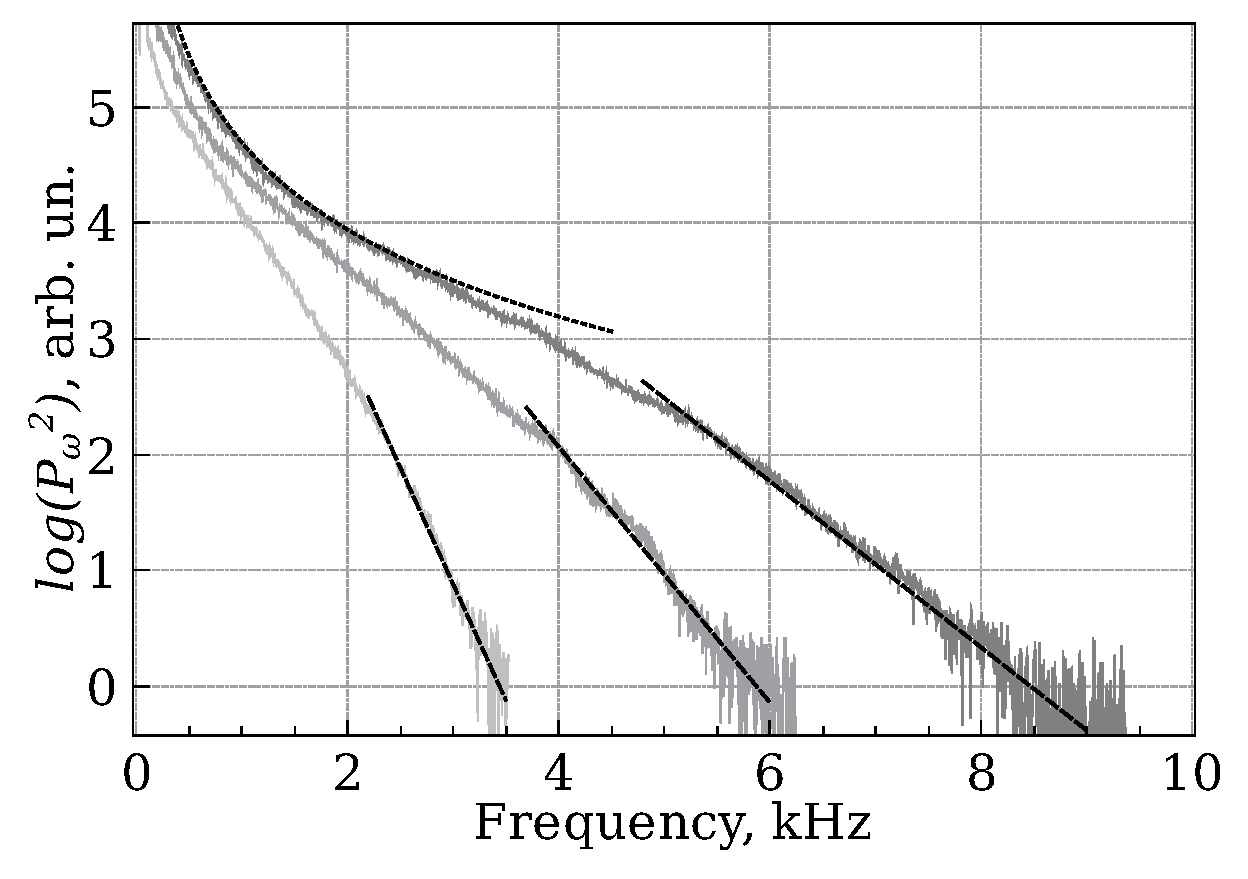
\includegraphics [scale=0.8] {article1/spectra_log.eps}
 \caption{Спектры $P^2_\omega$ для уровней накачки $V_p = 8$ В (светло серая линия), $16$ В (серая линия) и $26$ В (темно-серая линия) в полулогарифмическом масштабе. Линией из точек показан степенной закон $\sim \omega^{-2.8}$, пунктирной линией - подгонка функцией $ \sim e^{-\omega/\omega_d}$. $\omega_d$ примерно равен 0.2, 0.4 и 0.6 для $V_p$ = 8, 16 и 26 В соответственно.} 
 \label{img:hydr_specrta_log} 
\end{figure}

	Характерная частота $\omega_d$ оцененная с помощью подгонки экспоненциального затухания в диссипативной области к экспериментальным данным, растет с увеличением амплитуды возбуждающей силы. Для измерения уровня возбуждения использовался отклик поверхности $\eta_0$, а именно абсолютное значение $P_\omega$ на частоте 53 Гц (положение максимума распределения $P_\omega^2$ внутри области накачки). Величина $\eta_0$ прямо пропорциональна средней высоте волны на той же самой частоте. На рис. \ref{img:hydr_wd} показано, что зависимость граничной частоты от величины возбуждения может быть описана степенным законом $\omega_d(\eta_0) \sim	\eta_0^m$ со значение показателя $m = 0.85 \pm 0.05$. Необходимо заметить, что подгонка экспоненциальных спектров с помощью "квази-Планка" с малым ненулевым $s$ ($|s| \le 2$) слабо влияет на полученный параметр $\omega_d$ (меньше чем на 20\%). Однако эта поправка не изменит показатель степени $m$ в пределах погрешности.

	Наблюдаемый показатель $m \approx 0.85$ значительно отличается от ожидаемого $m = 12/5$ из параграфа \ref{subsect_hiFreqBound}. Стоит отметить, что в случае турбулентных каскадов, возбужденных монохроматической силой, измеренная граничная частота находится в хорошем соответствии с ожиданиями $\omega_d(\eta) \sim \eta^{1.3}$ \cite{Brazhnikov2001}.
	
\begin{figure}[ht] 
 \center
 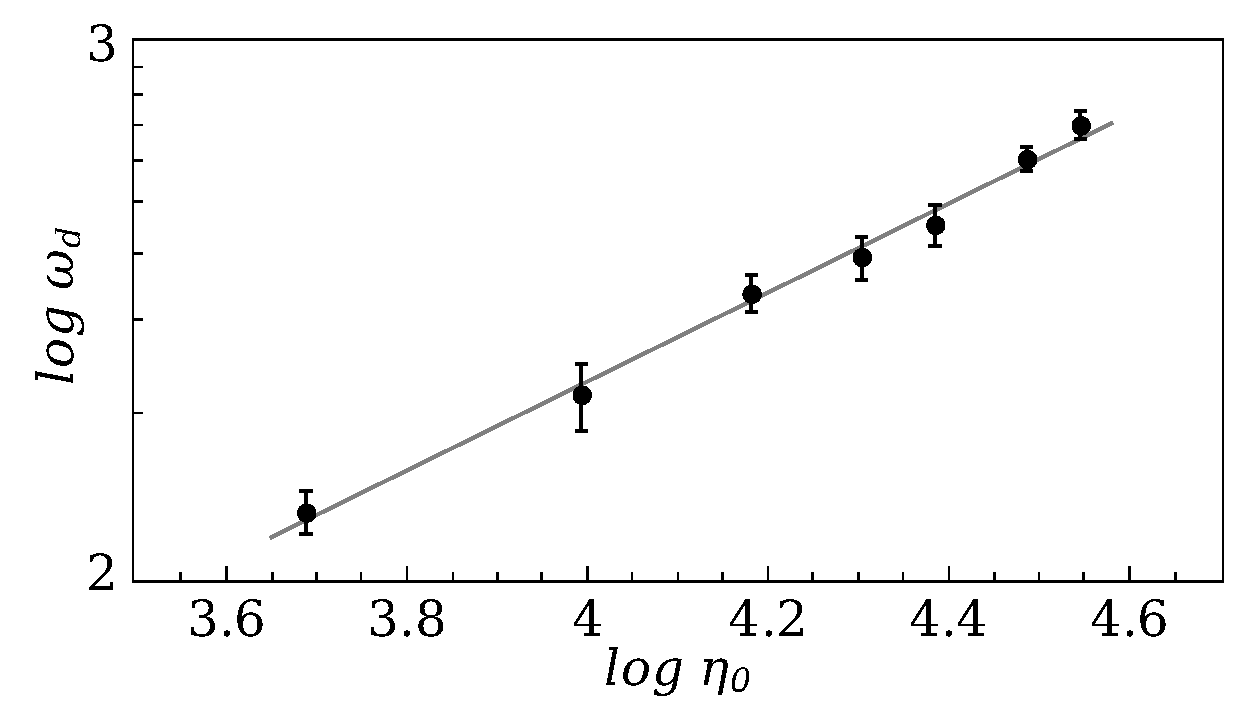
\includegraphics [scale=0.7] {article1/wd.eps}
 \caption{Зависимость частоты вязкого затухания диссипативной области $\omega_d$ (черные точки) от средней высоты низкочастотной волны $\eta_0$, сплошная линия - подгонка функцией $\eta_0^{0.85}$. } 
 \label{img:hydr_wd} 
\end{figure}
\section{Выводы}% \label{sect2_4}

 	Впервые наблюден переход от степенного спектра Колмогова-Захарова в инерционном интервале к “квазипланковскому” распределению $\omega^{-s}e^{-\omega/\omega_d}$ в области диссипации энергии в турбулентном распределении системы капиллярных волн. Экспоненциальный спад в области диссипации $\omega/\omega_d \gg 1$ соответствует теоретическому ожиданию и качественно соответствует численным вычислениям \cite{Ryzhenkova1990}. Граница вязкого затухания $\omega_d$ растет с увеличением амплитуды накачки и зависит от средней высоты волны $\eta_0$ на частоте накачки как $\omega_d \sim \eta^{0.85 \pm 0.05}$. Однако наблюденная зависимость отличается от ожидаемой, показатель степени почти в три раза больше, чем предсказанное значение.



\clearpage

           % Глава 2
%\section{Одиночное изображение} \label{sect2_1}
%
%\begin{figure}[ht] 
%  \center
%  \includegraphics [scale=0.27] {latex}
%  \caption{TeX.} 
%  \label{img:latex}  
%\end{figure}
%
%%\newpage
%%============================================================================================================================
%\section{Длинное название параграфа, в котором мы узнаём как сделать две картинки с общим номером и названием} \label{sect2_2}
%
%А это две картинки под общим номером и названием:
%\begin{figure}[ht]
%  \begin{minipage}[ht]{0.49\linewidth}
%    \center{\includegraphics[width=0.5\linewidth]{knuth1} \\ а)}
%  \end{minipage}
%  \hfill
%  \begin{minipage}[ht]{0.49\linewidth}
%    \center{\includegraphics[width=0.5\linewidth]{knuth2} \\ б)}
%  \end{minipage}
%  \caption{Очень длинная подпись к изображению, на котором представлены две фотографии Дональда Кнута}
%  \label{img:knuth}  
%\end{figure}
%
%Те~же~две картинки под~общим номером и~названием, но с автоматизированной нумерацей подрисунков посредством пакета \verb|subcaption|:
%\begin{figure}[ht]
%    \center{
%        \hfill
%        \subcaptionbox[List-of-Figures entry]{Первый подрисунок\label{img:knuth_2_1}} {\includegraphics[width=0.25\linewidth]{knuth1}}%
%        \hfill       
%        \subcaptionbox{Второй подрисунок\label{img:knuth_2_2}} {\includegraphics[width=0.25\linewidth]{knuth2}}
%        \hfill
%    }
%
%    Подрисуночный текст, описывающий обозначения, например. Согласно ГОСТ 2.105, пункт 4.3.1, располагается перед наименованием рисунка.
%    \caption{Очень длинная подпись к второму изображению, на котором представлены две фотографии Дональда Кнута} % Этот текст попадает в названия рисунков в списке рисунков
%    \label{img:knuth_2}
%\end{figure}
%
%
%На рисунке~\ref{img:knuth_2_1} показан Дональд Кнут без головного убора. На рисунке~\ref{img:knuth_2}\subref*{img:knuth_2_2}  показан Дональд Кнут в головном уборе.
%
%%\newpage
\chapter{Турбулентный капиллярный каскад вблизи края инерционного интервала на поверхности квантовой жидкости}
\section{Экспериментальная методидка} %\label{sect2_1}

Экспериментальная установка, схематично представленная на рис. \ref{img:water_setup}, состоит из виброплатформы 1, установленной на ней экспериментальной ячейки с водой 2 и системы регистрации колебаний 3, 4.
\begin{figure}[ht] 
  \center
  \includegraphics [scale=0.4] {article2/pic_01.jpg}
  \caption{Схема эксперимента: 1 – виброплатформа; 2 – сосуд с водой; 3 – лазер; 4 – фотоприемник.} 
  \label{img:water_setup}  
\end{figure}


Экспериментальные ячейки имели форму стакана диаметром от 65 до 130 мм и глубиной 10 мм, а также прямоугольника со сторонами 49 $\times$ 50 мм и глубиной 10 мм. Вода наливается выше края стенок стакана так, чтобы образовался выгнутый мениск. При вертикальных осцилляциях ячейки равновесный радиус мениска меняется в зависимости от ускорения ячейки, благодаря чему возбуждаются колебания поверхности воды. Волны на поверхности воды возбуждали, подавая переменное электрическое напряжение с цифрового генератора на вход виброплатформы. Использовали следующие виды накачек: монохроматическую на резонансной частоте, узкополосную с шириной полосы около 1 Гц и широкополосную 30–50 Гц. Под амплитудой накачки А в случае монохроматического возбуждения понимается амплитуда электрического сигнала, подаваемого на виброплатформу. В случае узкополосной или широкополосной накачки за амплитуду А принимается среднеквадратичное значение электрического сигнала, подаваемого на виброплатформу. От- метим, что высота волны основной гармоники на поверхности воды прямо пропорциональна амплитуде А (ускорению ячейки в вертикальном направлении) при монохроматической накачке.

Для регистрации колебаний поверхности воды была использована система, ранее описанная в \cite{Brazhnikov_IET}. Скользящий под небольшим углом лазерный луч падает на поверхность воды и отражается от нее. Мощность отраженного лазерного луча зависит от угла отражения. Поэтому присутствие волн на поверхности приводит к временным вариациям мощности отраженного луча $P(t)$. Отраженный луч фокусируется на фотодетектор, электрический сигнал с которого оцифровывается и записывается в память компьютера.

Регистрация волн на поверхности воды происходит в режиме “широкого луча”, т.е. характерная длина волн на поверхности воды много меньше размера пятна лазерного луча. В этом режиме мощность, регистрируемая фотодетектором, является интегральной характеристикой формы поверхности. В \cite{Brazhnikov_IET} показано, что при равномерном распределении световой мощности по лазерному пятну на поверхности жидкости парная корреляционная функция $I_\omega$ прямо пропорциональна квадрату компоненты Фурье мощности $P_\omega^2$ отраженного лазерного луча:
\begin{equation}
% \label{eq:disper}
I_\omega = P_\omega^2.
\end{equation}

\begin{figure}[ht] 
  \center
  \includegraphics [scale=0.2] {article2/pic_02.jpg}
  \caption{Распределение по частотам и амплитудам волн на поверхности воды в цилиндрической ячейке диаметром 65 мм. Справа приведена шкала амплитуд в произвольных единицах.} 
  \label{img:water_freq_scan}  
\end{figure}


На рис. \ref{img:water_freq_scan} показано экспериментальное распределение амплитуд волн по частоте при возбуждении волн в ячейке диаметром 65 мм, глубиной 10 мм монохроматической силой на фиксированной частоте накачки $f_p$. Частота накачки увеличивается от 46 до 90 Гц с шагом 0.1 Гц. По оси абсцисс отложена частота в герцах, а по оси ординат номер регистрируемой гармоники $N$ с частотой $N f_p$.
Оценка показывает, что в интервале частот от 45 до 90 Гц расстояние между резонансными пи- ками превосходит ширину пиков, вязкое уширение резонансных пиков $2\nu\omega^{4/3}(\rho/\sigma)^{2/3}$ ($\rho$ – плотность, $\nu$ – кинематическая вязкость, $\sigma$ – коэффициент поверхностного натяжения воды), т.е. спектр поверхностных колебаний в этом диапазоне частот является дискретным.
На рис. \ref{img:water_signal_example} приведен пример записи сигнала, регистрируемого фотодетектором при монохроматическом возбуждении волн на частоте 46 Гц в цилиндрической ячейке. Отметим, что основные вариации мощности отраженного лазерного луча обусловлены колебаниями поверхности воды на частоте накачки.

\begin{figure}[ht] 
  \center
  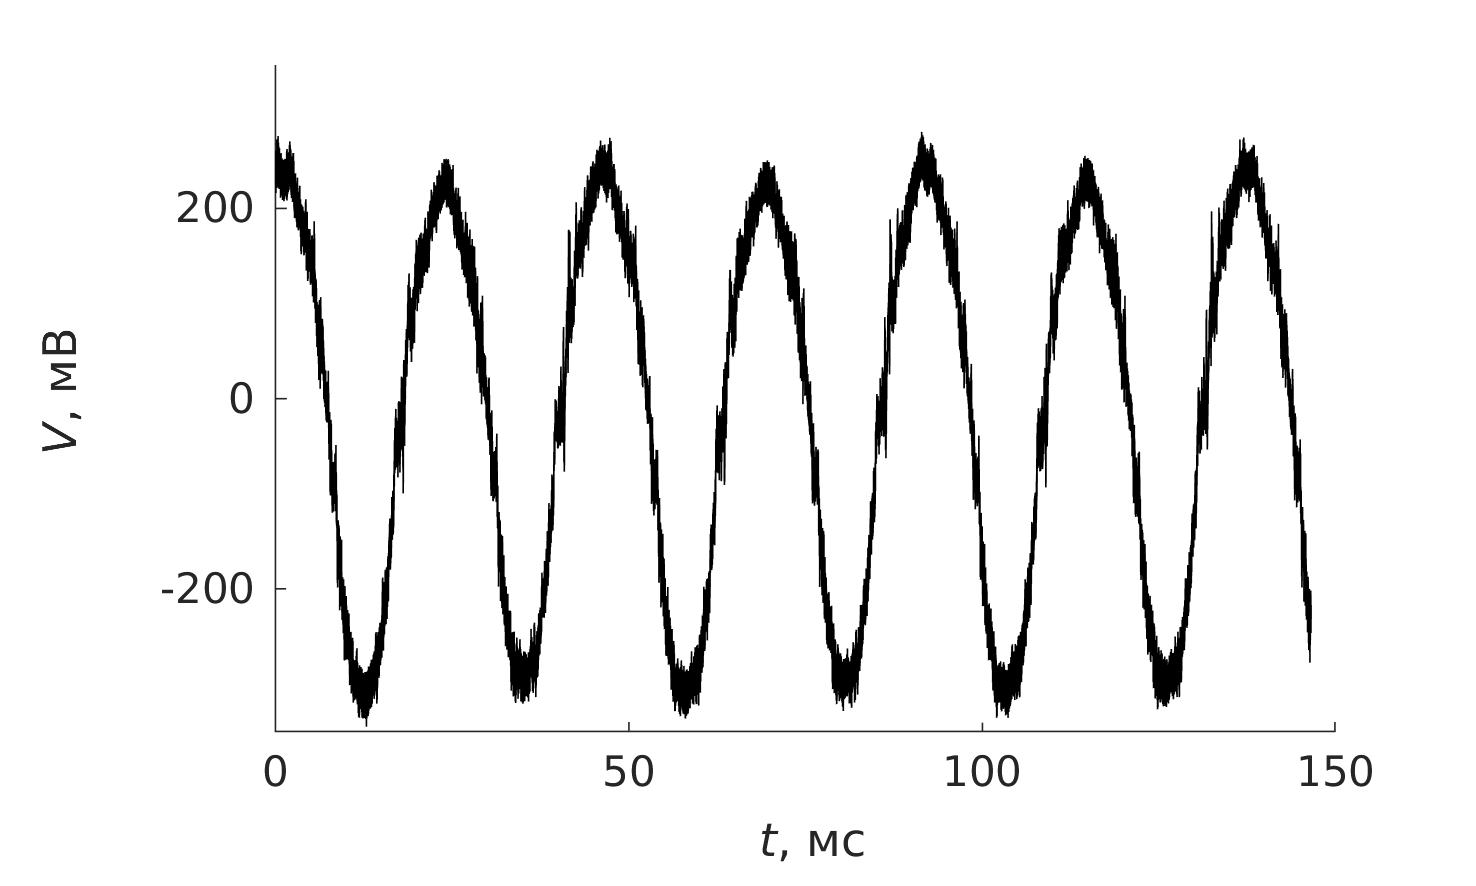
\includegraphics [scale=0.2] {article2/pic_03.jpg}
  \caption{Пример записи сигнала с фотодетектора при возбуждении поверхности воды монохроматической накачкой на частоте 46 Гц в ячейке диаметром 65 мм.} 
  \label{img:water_signal_example}  
\end{figure}




\section{Экспериментальные результаты}% \label{sect2_2}

На рис. \ref{img:water_spectrum} приведен спектр $P^2_\omega$ , полученный фурье-преобразованием сигнала, показанного на рис. \ref{img:water_signal_example}. Отметим особенности на этом распределении. Самый большой пик, расположенный слева на шкале частот, соответствует частоте возбуждающей монохроматической силы $f_b$ = 46 Гц. Стрелкой на спектре отмечен край инерционного интервала $f_b$. На частотах выше $f_b$ располагается диссипативная область, в которой турбулентный поток энергии быстро затухает. В диапазоне между областью накачки и краем инерционного интервала располагаются пики, соответствующие резонансам, возникшим в результате трехволнового взаимодействия c частотами, кратными $f_b$. Видно, что максимумы пиков в спектре в пределах инерционного интервала хорошо ложатся на прямую линию, которая соответствует степенному закону распределения с показателем степени, близким к –3.
\begin{figure}[ht] 
  \center
  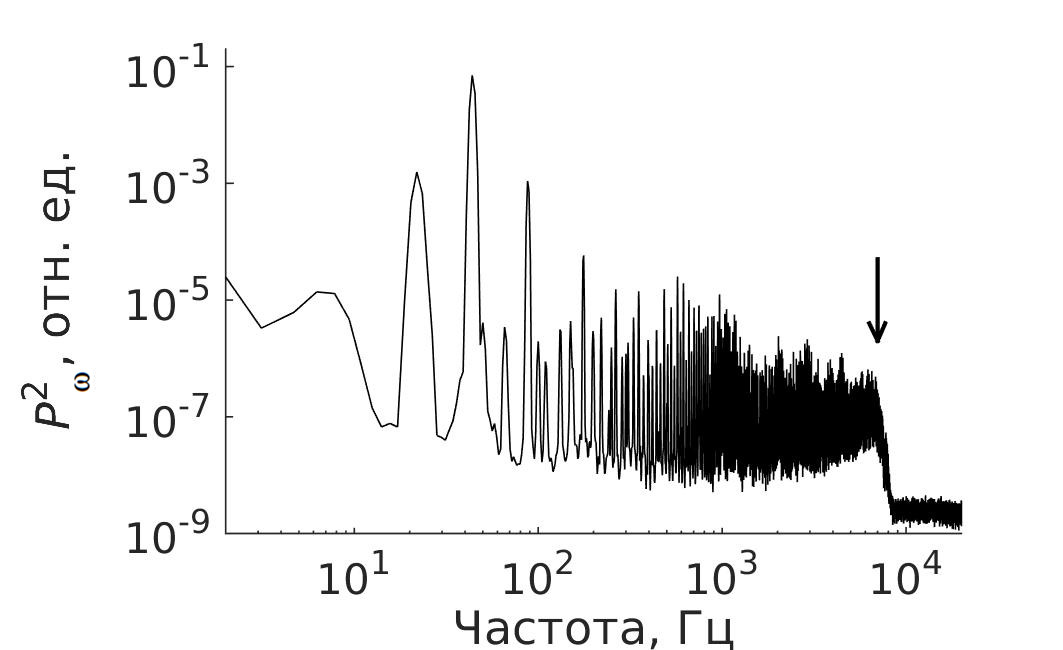
\includegraphics [scale=0.3] {article2/pic_04.jpg}
  \caption{Турбулентный каскад на поверхности воды в ячейке диметром 65 мм. Монохроматическая накачка на частоте 46 Гц.} 
  \label{img:water_spectrum}  
\end{figure}



С увеличением амплитуды возбуждающей силы положение высокочастотного края инерционного интервала $f_b$ сдвигается в сторону высоких частот. Частота $f_b$ определяется по компенсированным спектрам $P_\omega^2/\omega^\gamma$. Показатель степени $gamma$ подбирается так, чтобы в инерционным интервале спектр $P_\omega^2/\omega^\gamma$ не зависел от частоты. Значение $f_b$ определяется как частота, при которой отклонение $P_\omega^2/\omega^\gamma$ от плоского спектра составляет 50%
\section{Высокочастотный край инерционного интервала}% \label{sect2_3}

Анализ зависимостей $f_b(А)$ показывает, что показатель степени $\beta$ зависит от амплитуды возбуждающей силы. На рис. \ref{img:water_ampl_scan} приведено распределение волн по частотам и амплитудам, полученное при двух последовательных циклах увеличения и уменьшения амплитуды возбуждающей силы на частоте накачки, равной $f_p = 44$ Гц. Край инерционного интервала располагается на границе серого и черного цветов и возрастает по мере повышения амплитуды накачки. На рисунке хорошо видно, что при малых амплитудах накачки частота высокочастотного края инерционного интервала растет по закону немного сильнее линейного, т.е. $\beta > 1$ вплоть до 80-й гармоники частоты накачки. При больших амплитудах накачки показатель степени $\beta$ приближается к единице.

\begin{figure}[ht] 
  \center
  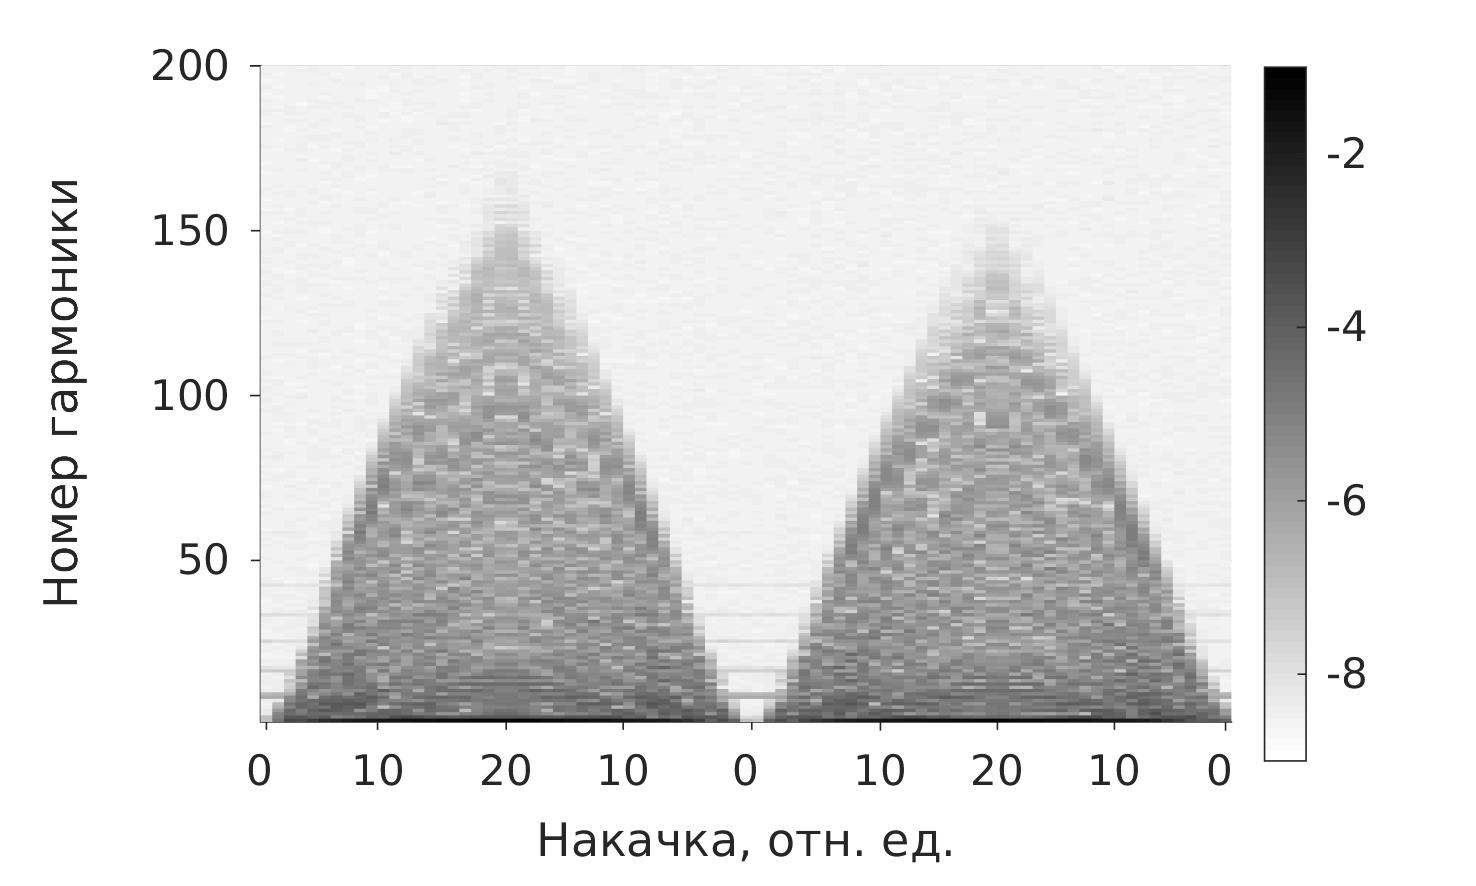
\includegraphics [scale=0.2] {article2/pic_05.jpg}
  \caption{Распределение волн по частоте и амплитуде колебаний при двух последовательных циклах увеличения и уменьшения амплитуды возбуждающей силы на частоте fp = 44 Гц. Амплитуда возбуждающей силы дана в произвольных единицах. Диаметр ячейки равнялся 65 мм.} 
  \label{img:water_ampl_scan}  
\end{figure}

На рис. \ref{img:water_fb_mono} в логарифмическом масштабе приведены зависимости частоты края инерционного интервала $f_b$ от амплитуды монохроматической накачки, полученные в цилиндрической ячейке диаметром 65 мм при накачке на частоте 45.5 Гц, в цилиндрической ячейке диаметром 130 мм при накачке на частоте 44 Гц. Видно, что полученные точки $f_b$ на графиках в логарифмических координатах хорошо ложатся на прямую линию, что соответствует степенной зависимости частоты края инерционного интервала от амплитуды накачки $f_b \sim А^\beta$. Экспериментально полученные значения показателя степени $\beta$ лежат в интервале от $1.3 \pm 0.2$ для всех цилиндрических ячеек. Отметим, что тео ретическое значение $\beta$ равно 4/3 для монохроматической накачки [F2]. Таким образом, можно заключить, что экспериментальные значения находятся в хорошем согласии с теоретической оценкой.

\begin{figure}[ht]
  \begin{minipage}[ht]{0.49\linewidth}
    \center{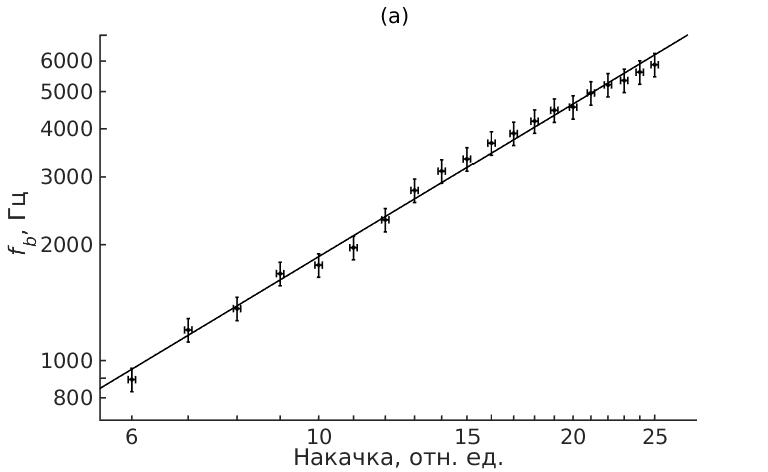
\includegraphics[width=1\linewidth]{article2/pic_06a.jpg} \\ а)}
  \end{minipage}
  \hfill
  \begin{minipage}[ht]{0.49\linewidth}
    \center{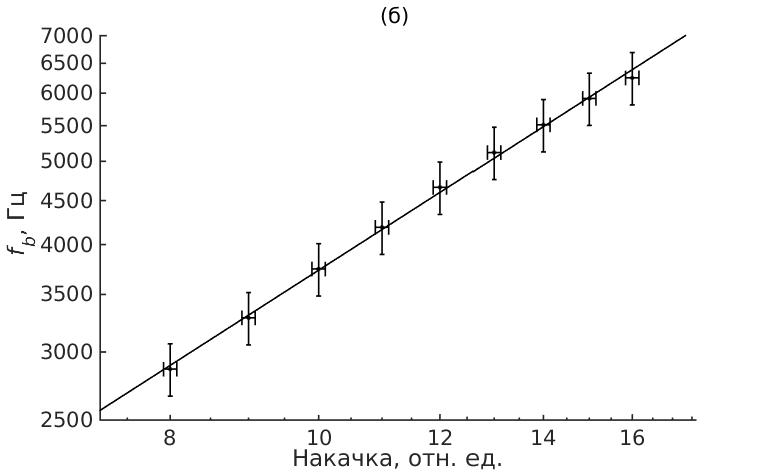
\includegraphics[width=1\linewidth]{article2/pic_06b.jpg} \\ б)}
  \end{minipage}
  \caption{Зависимость высокочастотного края инерционного интервала от амплитуды монохроматической накачки в цилиндрических ячейках диаметром 65 мм, $f_p$ = 45.5 Гц (а) и 130 мм, $f_p$ = 44.0 Гц (б).}
  \label{img:water_fb_mono}  
\end{figure}

При переходе от монохроматической к широкополосной накачке также наблюдаются хорошие степенные зависимости $f_b \sim А^\beta$ в широком интервале амплитуд возбуждающей силы, но показатель степени $\beta$ меньше, чем в случае монохроматической накачки.

\begin{figure}[ht]
  \begin{minipage}[ht]{0.49\linewidth}
    \center{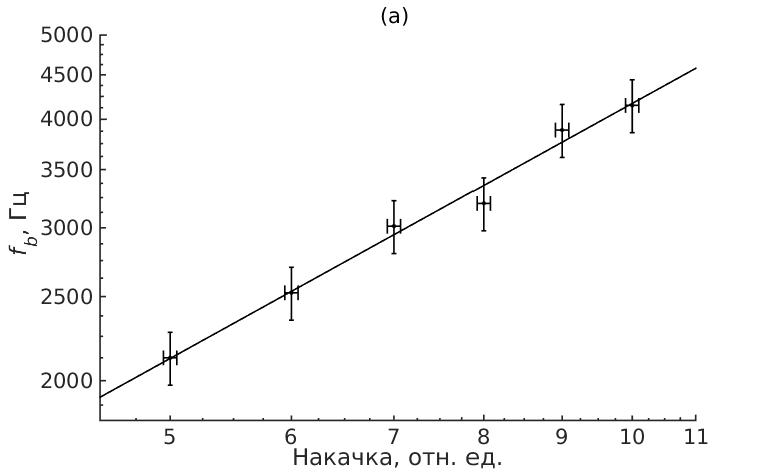
\includegraphics[width=1\linewidth]{article2/pic_07a.jpg} \\ а)}
  \end{minipage}
  \hfill
  \begin{minipage}[ht]{0.49\linewidth}
    \center{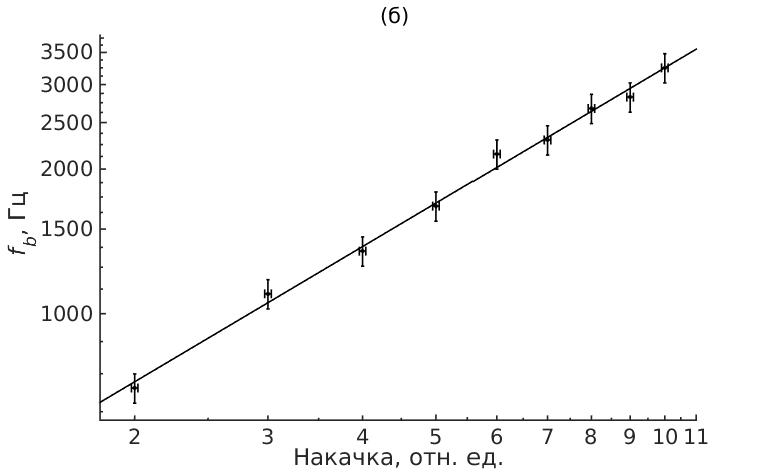
\includegraphics[width=1\linewidth]{article2/pic_07b.jpg} \\ б)}
  \end{minipage}
  \caption{Зависимость высокочастотного края инерционного интервала $f_b$ от амплитуды широкополосной накачки в интервале 30–50 Гц в цилиндрических ячейках диаметром 65 (а) и 130 мм (б).}
  \label{img:water_fb_wide}  
\end{figure}

На рис. \ref{img:water_fb_wide} приведены в логарифмическом масштабе зависимости частоты края инерционного интервала от амплитуды широкополосной накачки для двух ячеек. Видно, что экспериментальные точки хорошо описываются степенными функциями амплитуды. Показатель степени $\beta$ изменяется от 1.32 в ячейке диаметром 65 мм до 1.14 в ячейке диаметром 130 мм, в среднем $\beta = 1.23 \pm 0.09$.

Также как и в случае монохроматической накачки экспериментальные точки на графиках хорошо ложатся на прямую линию, что соответствует степенной зависимости частоты края инерционного интервала от амплитуды накачки. Отметим, что полученные величины показателя степени $beta$ составляют в среднем $1.10 \pm 0.15$ и значительно отличаются от теоретического значения, равного 12/5 \cite{Ryzhenkova}.
Чтобы убедиться, что полученные степенные зависимости $f_b(А)$ не являются особенностью волн в цилиндрической 
ячейке, эксперименты были повторены на почти квадратной ячейке со сторонами $49 \times 50$ мм. На рис. \ref{img:water_fb_rect} приведены зависимости частоты высокочастотного края инерционного интервала $f_b$ от амплитуды монохроматической и широкополосной возбуждающей силы. Видно, что в этих случаях зависимость $f_b(А)$ можно также описать степенной функцией с показателем степени, равным $0.95 \pm 0.03$. Оказалось, что присутствие вихрей на поверхности не оказывает существенного влияния на волновую турбулентность.
\begin{figure}[ht]
  \begin{minipage}[ht]{0.49\linewidth}
    \center{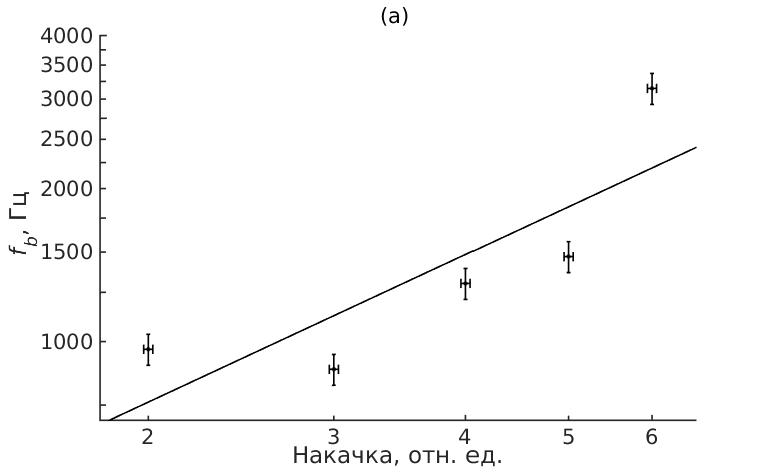
\includegraphics[width=1\linewidth]{article2/pic_08a.jpg} \\ а)}
  \end{minipage}
  \hfill
  \begin{minipage}[ht]{0.49\linewidth}
    \center{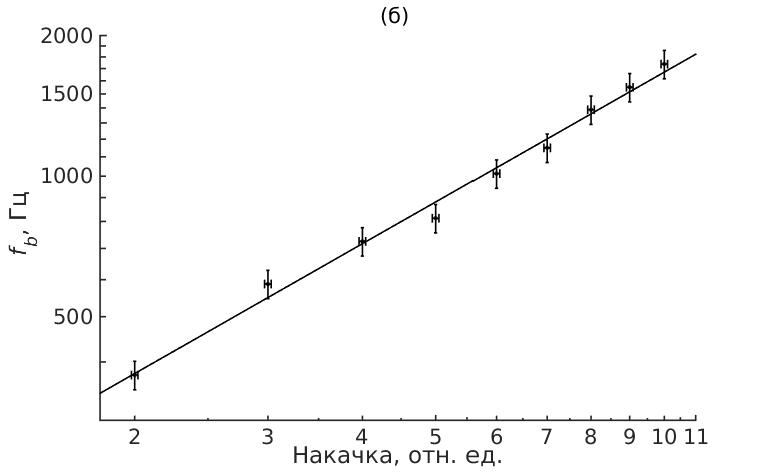
\includegraphics[width=1\linewidth]{article2/pic_08b.jpg} \\ б)}
  \end{minipage}
  \caption{Зависимость частоты высокочастотного края инерционного интервала $f_b$ от амплитуды монохроматической (а) и широкополосной (б) накачки в ячейке размерами 49 x 50 мм.}
  \label{img:water_fb_rect}  
\end{figure}

Отметим, что при узкополосной накачке (ширина полосы ~1 Гц) в полученных спектрах $P^2_\omega$ край инерционного интервала слабо выражен, вследствие чего зависимость края инерционного интервала от амплитуды накачки установить не удается.

\section{Характреная частота затухания}% \label{sect2_3}
Как отмечалось выше, на частотах выше $f_b$ турбулентный каскад затухает в результате вязких потерь. На рис. \ref{img:water_fd_mono} в двойных логарифмических координатах приведены зависимости характерной частоты $f_d$ от амплитуды монохроматической накачки для двух ячеек. Отметим, что в ячейке диаметром 65 мм (рис. \ref{img:water_fd_mono}а) частота $f_d$ возрастает по степенному закону при повышении амплитуды возбуждающей силы до значения А = 12. В ячейке большего диаметра наблюдается монотонное повышение характерной частоты с ростом уровня накачки. Приближение экспериментальных данных степенной зависимостью $f_d \sim А^\alpha$ дает следующее значения показателя степени $\alpha = 1.18$ для ячейки диаметром 65 мм на растущем участке и $\alpha = 1.38$ для ячейки диаметром 130 мм, в среднем $\alpha = 1.28 \pm 0.10$.

\begin{figure}[ht]
  \begin{minipage}[ht]{0.49\linewidth}
    \center{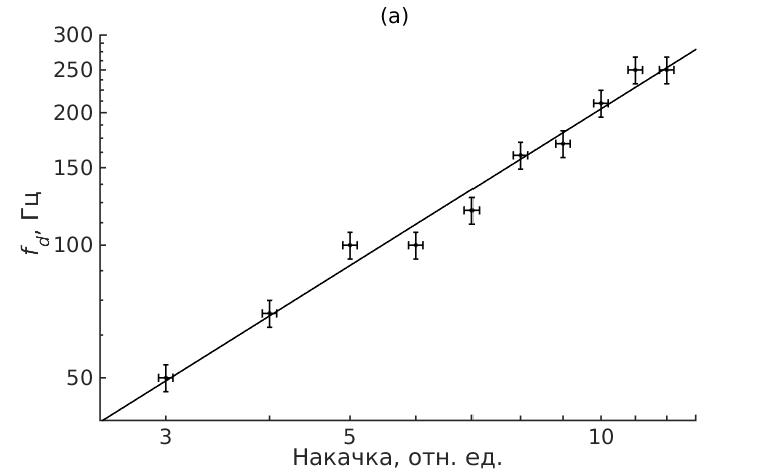
\includegraphics[width=1\linewidth]{article2/pic_09a.jpg} \\ а)}
  \end{minipage}
  \hfill
  \begin{minipage}[ht]{0.49\linewidth}
    \center{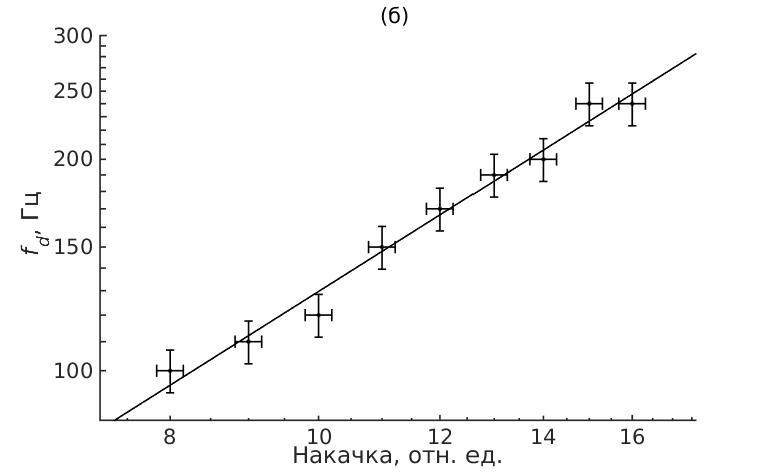
\includegraphics[width=1\linewidth]{article2/pic_09b.jpg} \\ б)}
  \end{minipage}
  \caption{Зависимость характерной частоты $f_d$ от амплитуды возбуждающей силы при монохроматической накачке на частоте 45.5 Гц в ячейке диаметром 65 мм (а) и на частоте 44.0 Гц в ячейке диаметром 130 мм (б).}
  \label{img:water_fd_mono}  
\end{figure}

На рис. \ref{img:water_spectra_linear} показано распределение $P^2_\omega$ в полулогарифмических координатах при широкополосной накачке в диапазоне 30–50 Гц, полученное в ячейке диаметром 65 мм. Амплитуды накачки в относительных единицах составляют 3:7:10. Стрелками на каждом спектре показано положение края инерционного интервала $f_b$, которое составляет 650, 2500 и 4300 Гц соответственно. На частотах выше $f_b$ в диссипативной области наблюдается экспоненциальное затухание. Для наглядности на рисунке проведены прямые линии, подчеркивающие экспоненциальные зависимости $P^2_\omega$. Характерные частоты, рассчитанные по зависимостям (2) для распределений, показанных на рис. \ref{img:water_fb_rect}, составляют 430, 1050, 1550 Гц соответственно.

\begin{figure}[ht] 
  \center
  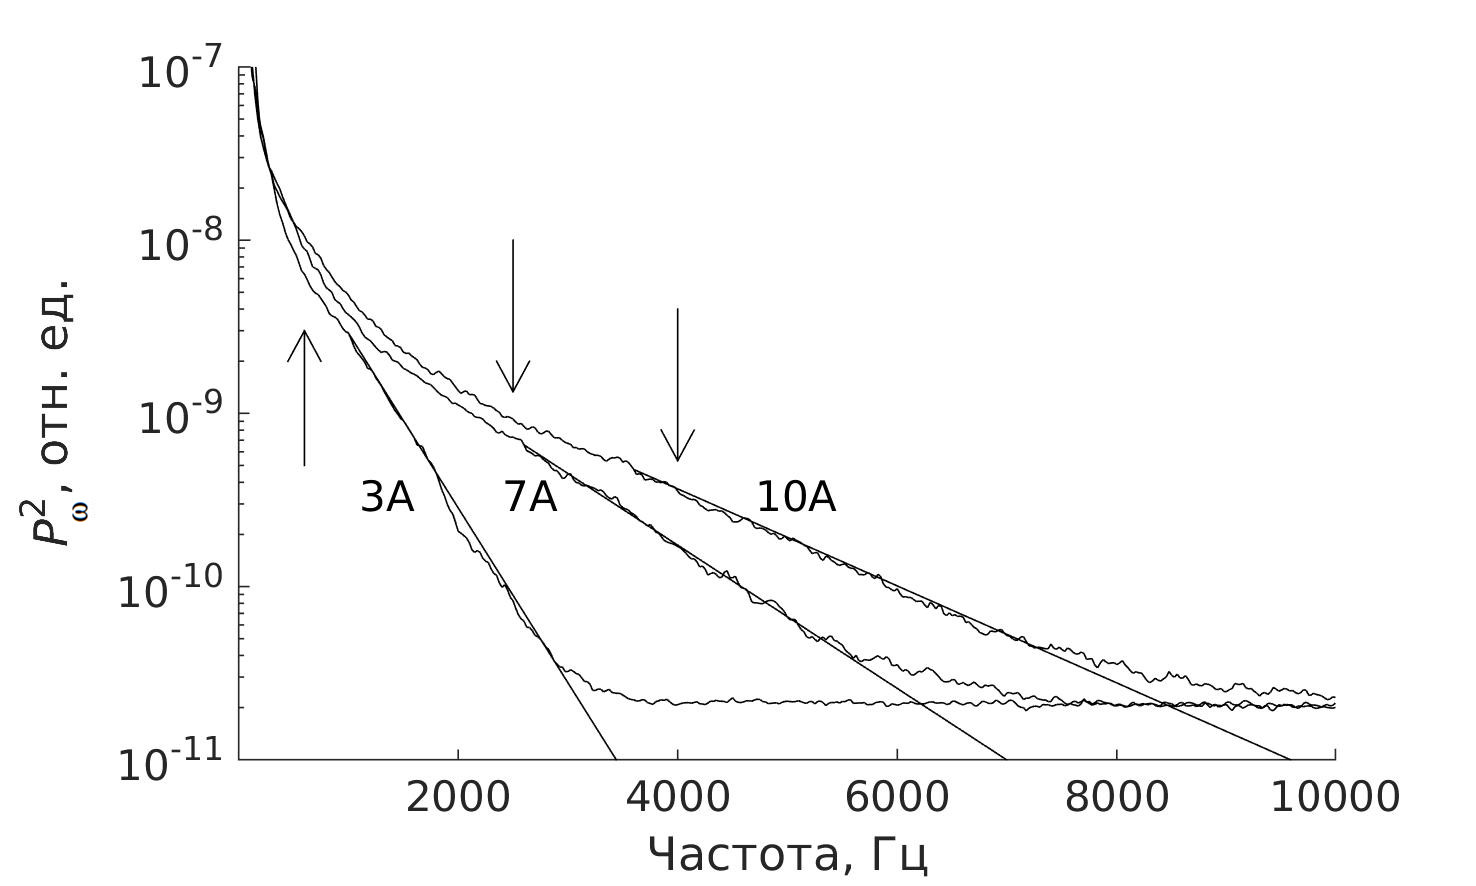
\includegraphics [scale=0.2] {article2/pic_10.jpg}
  \caption{Турбулентные распределения на поверхности воды в ячейке диаметром 65 мм при накачке в диапазоне 30–50 Гц. Амплитуды накачки в относительных единицах приведены у кривых.} 
  \label{img:water_spectra_linear}  
\end{figure}


В случае широкополосной накачки зависимость частоты $f_d$ от амплитуды накачки является монотонной. На рис. \ref{img:water_fd_wide} приведены в логарифмическом масштабе зависимости $f_d$ от амплитуды широкополосной накачки в двух ячейках. Видно, что точки на графике хорошо ложатся на прямую линию, соответствующую степенной зависимости от амплитуды с показателем степени, близким к значениям, полученным по зависимостям частоты края инерционного интервала от амплитуды накачки. Полученные значения $\alpha$ близки к 1.1.

\begin{figure}[ht]
  \begin{minipage}[ht]{0.49\linewidth}
    \center{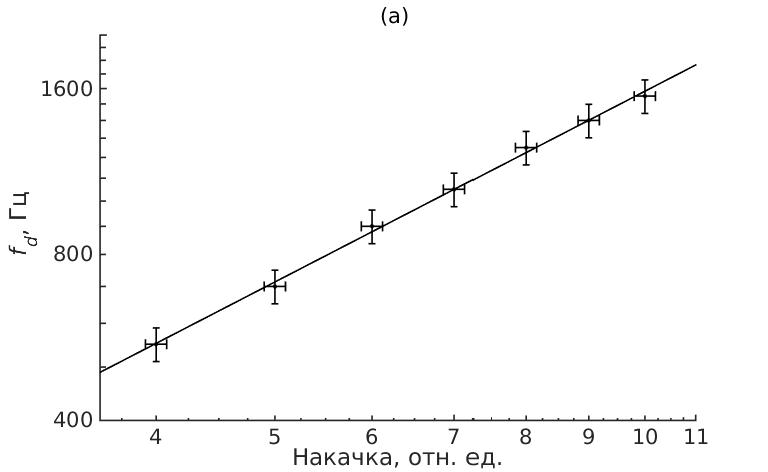
\includegraphics[width=1\linewidth]{article2/pic_11a.jpg} \\ а)}
  \end{minipage}
  \hfill
  \begin{minipage}[ht]{0.49\linewidth}
    \center{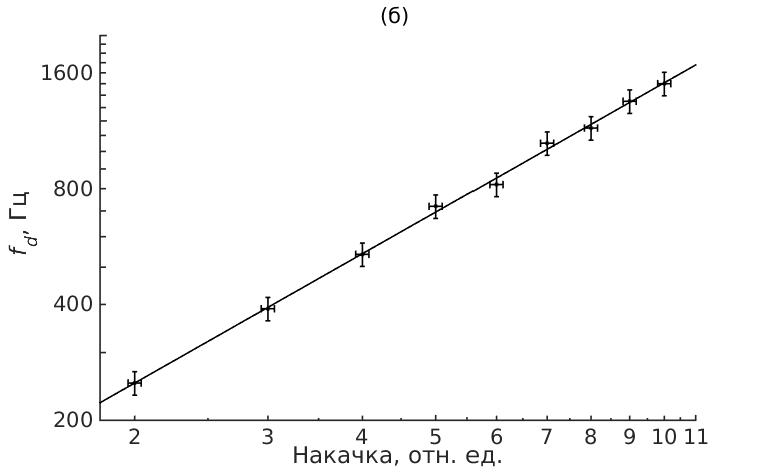
\includegraphics[width=1\linewidth]{article2/pic_11b.jpg} \\ б)}
  \end{minipage}
  \caption{Зависимость характерной частоты $f_d$ от амплитуды возбуждающей силы при широкополосной накачке на частотах от 30 до 50 Гц в ячейке диаметром: а – 65; б – 130 мм.}
  \label{img:water_fd_wide}  
\end{figure}


\section{Обсуждение}% \label{sect2_3}

Экспериментальные данные свидетельствуют, что амплитудные зависимости частоты высокочастотного края инерционного интервала $f_b$ можно хорошо описать степенными функциями амплитуды $A^\beta$. Показатель степени при монохроматической накачке составляет в среднем $\beta = 1.23 \pm 0.09$, что близко к теоретической оценке $\beta = 4/3$. Амплитудная зависимость характерной частоты экспоненциального затухания турбулентного каскада описывается степенной функцией с показателем, равным $\alpha = 1.28 \pm 0.10$ Поэтому можно утверждать, что в случае монохроматической накачки частота $f_b$ прямо пропорционально $f_d$, $f_b = m f_d$. Значение коэффициента пропорциональности m составляет 4–5, т.е. характерная частота $f_d$ в несколько раз меньше частоты края инерционного интервала.

При широкополосной накачке показатели степени составляют в среднем $\beta = 1.10 \pm 0.15$ и $\alpha = 1.12 \pm 0.03$, т.е. они практически совпадают. Поэтому можно полагать, что $f_b = n f_d$, а значение n составляет 3–4. Это означает, что гармоники из диссипативной области как при монохроматической накачке, так и при широкополосном возбуждении взаимодействуют, в основном, с модами, расположенными в пределах инерционного интервала [F1], но ниже частоты его края. Как близко эти моды расположены к краю инерционного интервала, установить сложно, но они значительно выше частоты накачки $f_p$.
Отметим, что в экспериментах со сверхтекучим гелием при монохроматической накачке характерная частота $f_d$ была близка к частоте накачки $f_p$ [F2] и меньше частоты края инерционного интервала в десятки раз. В то же время при широкополосной накачке в экспериментах с жидким водородом характерная частота $f_d$ была только в несколько раз ниже частоты высокочастотного края инерционного интервала $f_b$ и значительно превосходила частоту накачки $f_p$ [F1].

Таким образом, можно полагать, что отношение частот $f_b$, $f_p$, $f_d$ в экспериментах на поверхности воды, как при широкополосной, так и монохроматической накачке и в экспериментах с широкополосной накачкой поверхности водорода качественно близки. Во всех этих случаях волны из диссипативной области взаимодействуют в основном с модами из инерционного интервала, вдали от областей накачки и края инерционного интервала.

Обратим внимание, что при высоких уровнях монохроматической накачки частота $f_b$ растет с повышением амплитуды по закону слабее линейного (рис. \ref{img:water_ampl_scan}). Остается непонятным расхождение в величине показателя степени $\beta$, полученного в эксперименте и оцененного из теории при широкополосном возбуждении волн. Отметим, что это разногласие наблюдается в экспериментах как с волнами на поверхности воды при различных методиках возбуждения поверхности \cite{Brazhnikov_EPL}, так и на поверхности жидкого водорода \cite{Brazhnikov_liq_hydr} и сверхтекучего гелия [F2]. Во всех этих экспериментах угловые амплитуды волн на частоте накачки одного порядка, что связано с особенностью методики регистрации отклонения поверхности жидкости от равновесного положения \cite{Brazhnikov_IET}, а кинематическая вязкость жидкостей изменяется примерно в 100 раз. То есть расхождения в значениях $\beta$ не связаны со свойствами жидкостей, а определяются другими причинами. Для прояснения этого во- проса нужны дополнительные исследования.

\section{Выводы} %\label{sect2_4}

В работе экспериментально показано, что при возбуждении турбулентного состояния на поверхности воды монохроматической или широкополосной накачкой высокочастотный край инерционного интервала и характерная частота в диссипативной области отличаются в несколько раз и качественно одинаково повышаются с ростом амплитуды накачки по степенному закону с показателем степени, близким к теоретически оцененному значению для монохроматического возбуждения. В случае широкополосной накачки наблюдается значительное расхождение между экспериментальными и теоретически оцененными значениями показателя $\beta$.

\clearpage

           % Глава 3


\chapter{Формирование вихревого течения капиллярными волнами на поверхности жидкости} \label{chapt3}

Не смотря на то, что было сделано немало работ \cite{VonKameke2011, Francois2014, Francois2013}, в которых исследованы статистические свойства турбулентной системы вихрей, возникших в результате неустойчивости Фарадея, детального исследования механизма генерации вихревого движения при развитии поверхностной неустойчивости выполнено не было. В данной главе приведены результаты экспериментального изучения процессов генерации вихревого движения капиллярными волнами при различных условиях возбуждения


\section{Экспериментальная методика}\label{sect3_2}
Закрепленный на виброплатформе сосуд цилиндрической или квадратной формы заполняли дистиллированной водой. Сторона квадратного сосуда составляла 50 мм, внутренний диаметр цилиндрического - 65 мм, глубина обоих сосудов 10 мм. Сосуд совершает гармонические колебания в вертикальном направлении с частотой $\omega_p$ и амплитудой $S$. В связанной с сосудом системе координат, на жидкость действует "фиктивная" сила тяжести с ускорением, равным сумме ускорения свободного падения $g$ и переменного ускорения сосуда $g \beta cos(\omega_p t)$, где $\beta = S \omega_p^2/g$ – безразмерная амплитуда переменного ускорения. На стенку сосуда прикреплен акселерометра, измеряющий ускорение сосуда. В главе \ref{p1_methodsExt} было показано, что в такой системе возможны два механизма рождения волн. Волны, возникающие благодаря изменению формы мениска, будут иметь относительно слабую амплитуда. А возбуждаться будут только радиальные моды.

При параметрическом же возбуждении поверхностных волн в цилиндрическом сосуде, кроме радиальных мод (\ref{eq:Bessel}), также могут возбуждаться и азимутальные моды.

Для декорирования течений на поверхности в воду насыпали стеклянные сферы диаметром 50 мкм, либо порошок из полиамида PA12 со средним диаметром частиц 25–30 мкм. Плотность стеклянных сфер была немного меньше плотности воды. Для получения изображения треков движения частиц на поверхности жидкости, частицы подсвечиваются фотовспышкой в стробоскопическом режиме и фотографируются с большой выдержкой. Для нахождения горизонтальной составляющей скорости течения жидкости поверхность с пробными частицами фотографировали с частотой около 5.5 кадра/с при длительности фотовспышки 1 мс. Поле скоростей определяли из парных изображений с помощью пакета PIVlab \cite{PIVlab, PIVlab1} для MatLab. 
Завихренность вычислялась из полученного поля скорости согласно формуле (\ref{eq:defVort}).


\section{Экспериментальные результаты и их обсуждение} \label{sect3_3} 
На рис. \ref{img:wave_rad} показана фотография поверхности воды в цилиндрическом сосуде, декорированной порошком из полиамида. При колебаниях виброплатформы на частоте 25 Гц с амплитудой ниже пороговой для данной частоты на поверхности жидкости возбуждается радиальная мода $n = 6$ с длиной волны $\lambda \approx 10$ мм. В зависимости от плотности и смачиваемости пробные частицы дрейфуют либо к узлам, либо к пучностям стоячих волн \cite{Lukaschuk2007}. На фотографии хорошо видны концентрические круги, сформированные частицами, которые собираются в узлах стоячей волны. Заметим, что на этом снимке вихревого движения не наблюдается. При постепенном увеличении амплитуды колебаний виброплатформы амплитуда колебаний поверхности жидкости плавно нарастает. При достижении некоторого значения амплитуды переменного ускорения $\beta$ наблюдается резкое усиление колебаний поверхности и возникает азимутальная мода (\ref{eq:Bessel}) с числом $m$ порядка 10. Эту амплитуду переменного ускорения принимали за пороговое значение $\beta_c$. Появление азимутальной моды сопровождается формированием вихревого движения на поверхности (рис. \ref{img:wave_az}). На фотографии отчетливо видна система из трех концентрических поясов вихрей. В каждом поясе содержится по 12 пар вихрей, вращающихся в противоположных направлениях. Наибольшие размеры имеют вихри внешнего пояса вблизи стенки сосуда. При дальнейшем увеличении амплитуды накачки возникают крупномасштабные течения, разрушающие концентрическое расположение вихрей.

\begin{figure}[ht] 
 \center
 \includegraphics [scale=1] {article3/pic_01.jpg}
 \caption{Фотография поверхности воды при колебаниях цилиндрического сосуда на частоте 25Гц с амплитудой меньшей критической для возбуждения параметрического резонанса} 
 \label{img:wave_rad} 
\end{figure}

\begin{figure}[ht] 
 \center
 \includegraphics [scale=1] {article3/pic_02.jpg}
 \caption{Распределение вихрей на поверхности воды в цилиндрическом сосуде. Частота колебаний сосуда $\omega_p/2\pi = 45$ Гц, амплитуда переменного ускорения $\beta = 0.36$, пороговое ускорение $\beta_c = 0.26$. Видна азимутальная мода n = 4, m = 6, $\omega/2\pi = 22$ Гц} 
 \label{img:wave_az} 
\end{figure}




Переход от цилиндрического сосуда к сосуду квадратной формы радикально отражается на условиях формирования системы вихрей. На рис. \ref{img:vort_square} показаны распределения завихренности на поверхности воды в квадратном сосуде при накачке на частоте 45.5 Гц до и после наступления параметрической неустойчивости, красный цвет на рисунке соответствует положительной завихренности, синий цвет - отрицательной завихренности, цветовая шкала, определяющая значение завихренности, так же представлена на рисунке. До порогового значения $\beta/\beta_c \approx 0.9$ наблюдается симметричная система небольших вихрей (рис. \ref{img:vort_square}a), которые образуют квадратную решетку с периодом, равным длине поверхностных волн на частоте 45.5 Гц ($\lambda \approx 6$ мм). Симметричная структура сохраняется и при незначительном превышении порогового значения ускорения, $\beta/\beta_c \approx 1.1$ (рис. \ref{img:vort_square}b). При дальнейшем повышении уровня накачки происходят слияние и укрупнение вихрей вследствие нелинейности.

\begin{figure}[ht]
 \begin{minipage}[ht]{0.49\linewidth}
 \center{\includegraphics[width=1\linewidth]{article3/pic_03a.eps} \\ а)}
 \end{minipage}
 \hfill
 \begin{minipage}[ht]{0.49\linewidth}
 \center{\includegraphics[width=1\linewidth]{article3/pic_03b.eps} \\ б)}
 \end{minipage}
 \caption{Завихренность $\Omega$ на поверхности воды в квадратном сосуде при разных амплитудах колебаний на частоте 45.5 Гц: до порога возникновения параметрической неустойчивости (амплитуда переменного ускорения $\beta$ = 0.4, a) и после развития параметрической неустойчивости ($\beta$ = 0.48, b). Пороговое ускорение $\beta_c$ = 0.44}
 \label{img:vort_square} 
\end{figure}


На рис. \ref{img:fft_square} приведены Фурье-образы вихревых структур, представленных на рис. \ref{img:vort_square}. При накачке с амплитудой, меньшей критического значения, на поверхности доминирует структура с обратным периодом $\approx$ 10 см$^{-1}$ (рис. \ref{img:fft_square}a) в обоих направлениях, что соответствует волновому числу волны на частоте накачки. На рис. \ref{img:fft_square} б, помимо первоначальной структуры, видна структура с обратным периодом около 6 см$^{-1}$, амплитуды Фурье которой в несколько раз превышают амплитуды Фурье первоначальной структуры. Возрастание периода решетки вихрей связано с появлением на поверхности воды стоячих волн с частотой $\omega_p/2$, длина волны которых совпадает с периодом вихревой структуры, возникающей при переходе через порог неустойчивости Фарадея. 


\begin{figure}[ht]
 \begin{minipage}[ht]{0.49\linewidth}
 \center{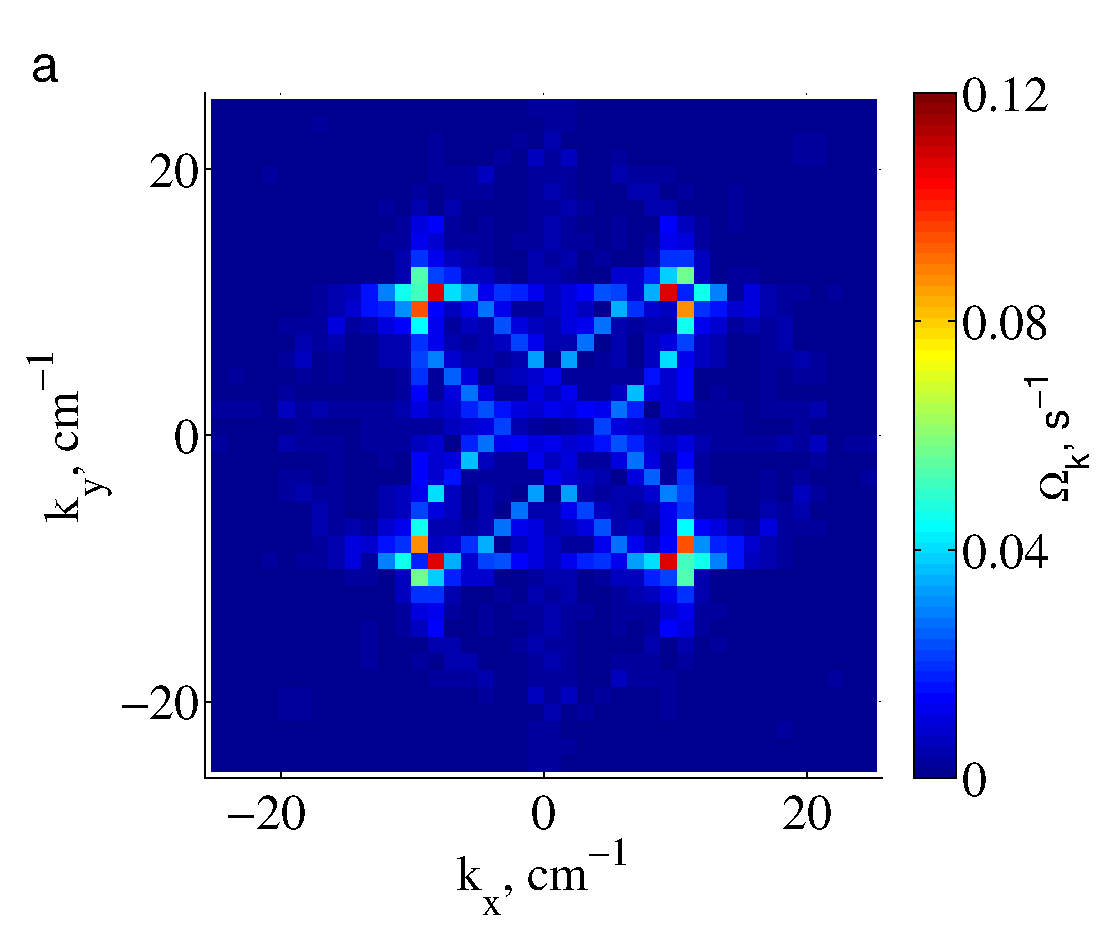
\includegraphics[width=1\linewidth]{article3/pic_04a.eps} \\ а)}
 \end{minipage}
 \hfill
 \begin{minipage}[ht]{0.49\linewidth}
 \center{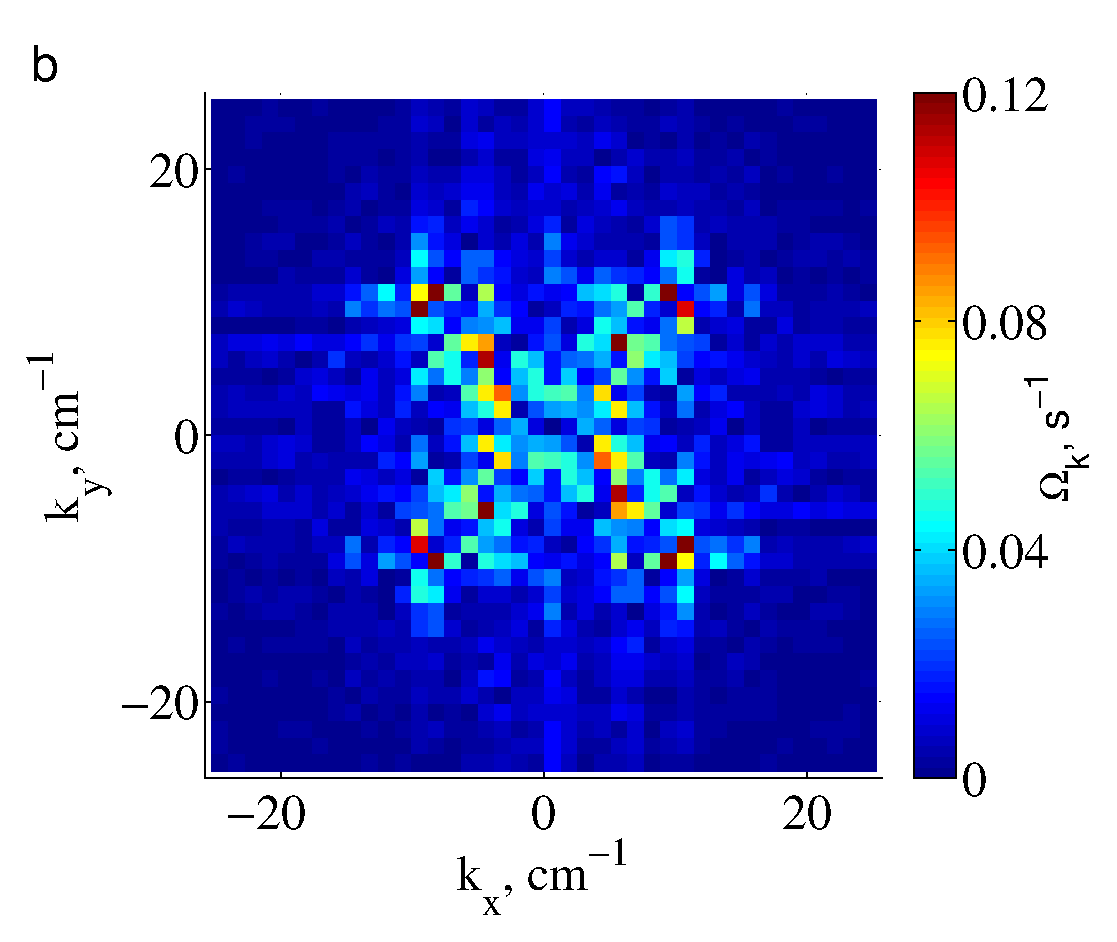
\includegraphics[width=1\linewidth]{article3/pic_04b.eps} \\ б)}
 \end{minipage}
 \caption{Фурье образ поля завихренности $\Omega_k$ на поверхности воды в квадратном сосуде при разных амплитудах колебаний на частоте 45.5 Гц: до порога возникновения параметрической неустойчивости (амплитуда переменного ускорения $\beta$ = 0.4, a) и после развития параметрической неустойчивости ($\beta$ = 0.48, б). Пороговое ускорение $\beta_c$ = 0.44}
 \label{img:fft_square} 
\end{figure}

Зависимость интегральной завихренности $|\Omega|$ движения на поверхности воды от амплитуды переменного ускорения $\beta$ в квадратном сосуде показана на рис. \ref{img:wave_ampl1}. При изменении амплитуды переменного ускорения $\beta$ от 0.11 до 0.55 модуль завихренности $|\Omega|$ возрастает почти на два порядка, причем его быстрый рост наблюдается при ускорениях выше порога параметрической неустойчивости. При накачках ниже порогового значения изменение модуля завихренности как функции амплитуды ускорения $\beta$ хорошо описывается степенной зависимостью $|\Omega| \sim \beta^{1.7}$. Поскольку при прочих равных условиях амплитуда возбуждаемых на поверхности стоячих волн $A$ прямо пропорциональна амплитуде переменного ускорения $\beta$, зависимость интегральной завихренности от амплитуды волн будет иметь удвоенный показатель степени $|\Omega| \sim \beta^{2}$ \cite{F6}. Отличие, по-видимому, вызвано неоднородностью поля завихренности: вблизи края сосуда она больше, чем в центре (рис. \ref{img:vort_square}a).

\begin{figure}[ht] 
 \center
 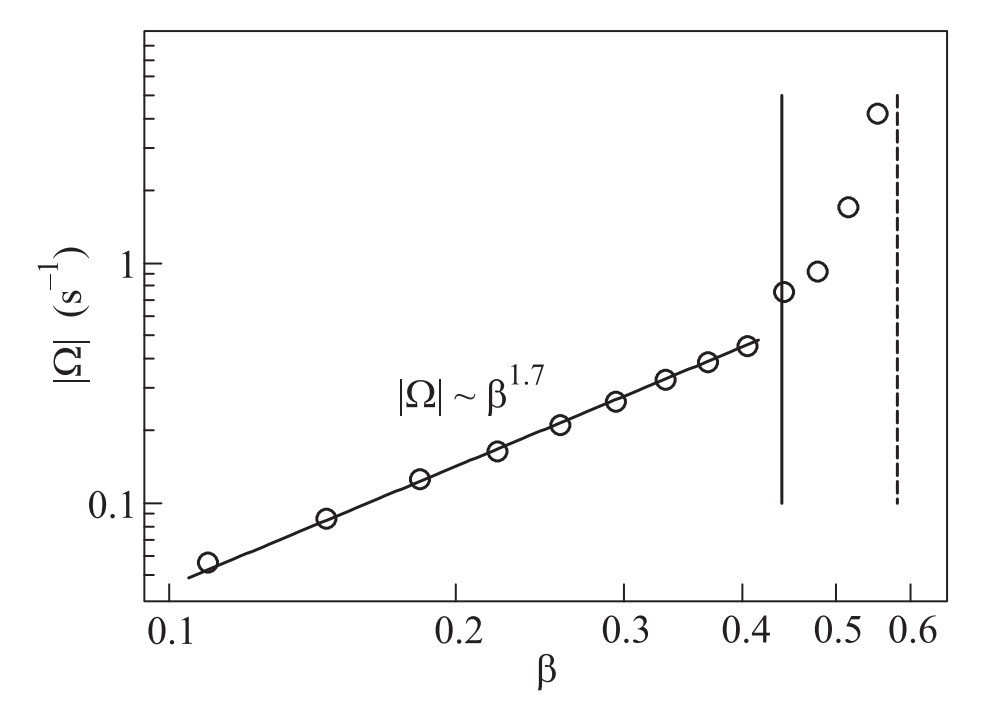
\includegraphics [scale=.4] {article3/pic12.jpg}
 \caption{Рис. 5. Зависимость суммарного модуля завихренности $| \Omega| = \int | \Omega(x,y)|dx dy$ на поверхности воды в квадратном сосуде от амплитуды переменного вертикального ускорения $\beta$. Сплошная вертикальная линия соответствует пороговой амплитуде переменного ускорения $\beta_c = 0.44$.} 
 \label{img:wave_ampl1} 
\end{figure}

Так как в квадратном сосуде вихревое движение наблюдается при амплитудах накачки значительно ниже порога параметрической неустойчивости, формирование вихревого движения здесь не может быть приписано особенностям параметрической неустойчивости Фарадея. Тот факт, что структуры вихревого и волнового движения коррелируют между собой, позволяет предположить, что волны непосредственно участвуют в формировании вихрей. Принципиальное отличие волн в квадратном сосуде, где вихри наблюдаются, начиная с самых малых амплитуд накачки, от волн в цилиндрическом сосуде, где вихри появляются только при достижении порога неустойчивости, связано с количеством одновременно возбуждаемых мод колебаний поверхности жидкости на фиксированной частоте. В квадратном сосуде ввиду симметричности всегда возбуждается пара мод (\ref{eq:waveStand}). В цилиндрическом сосуде две разные моды, радиальная и азимутальная, одновременно возбуждаются только после превышения порога параметрической неустойчивости. Можно предположить, что изменение симметрии цилиндрического сосуда, которое приведет к возбуждению азимутальных мод при амплитудах накачки, меньших порогового значения, также сделает возможным формирование вихревого движения при этих же амплитудах.

\begin{figure}[ht]
 \begin{minipage}[ht]{0.49\linewidth}
 \center{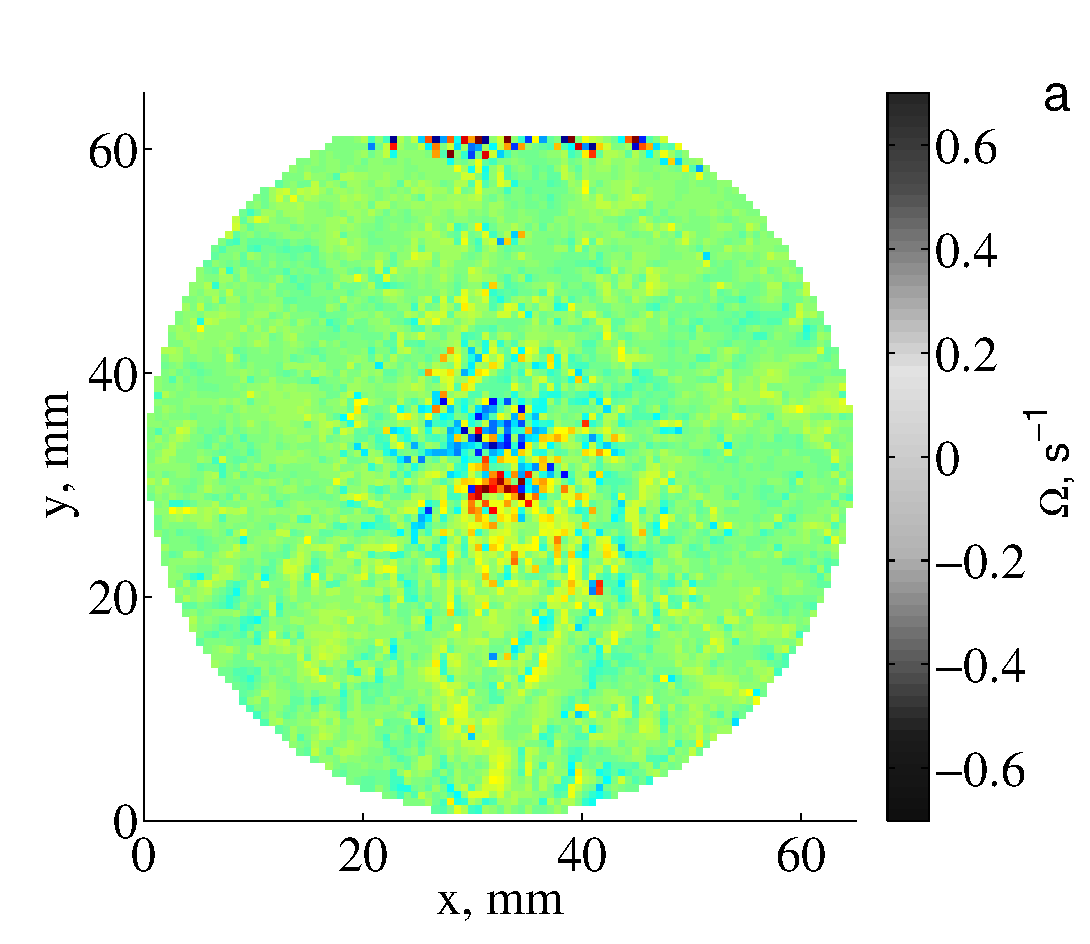
\includegraphics[width=1\linewidth]{article3/pic_06a.eps} \\ а)}
 \end{minipage}
 \hfill
 \begin{minipage}[ht]{0.49\linewidth}
 \center{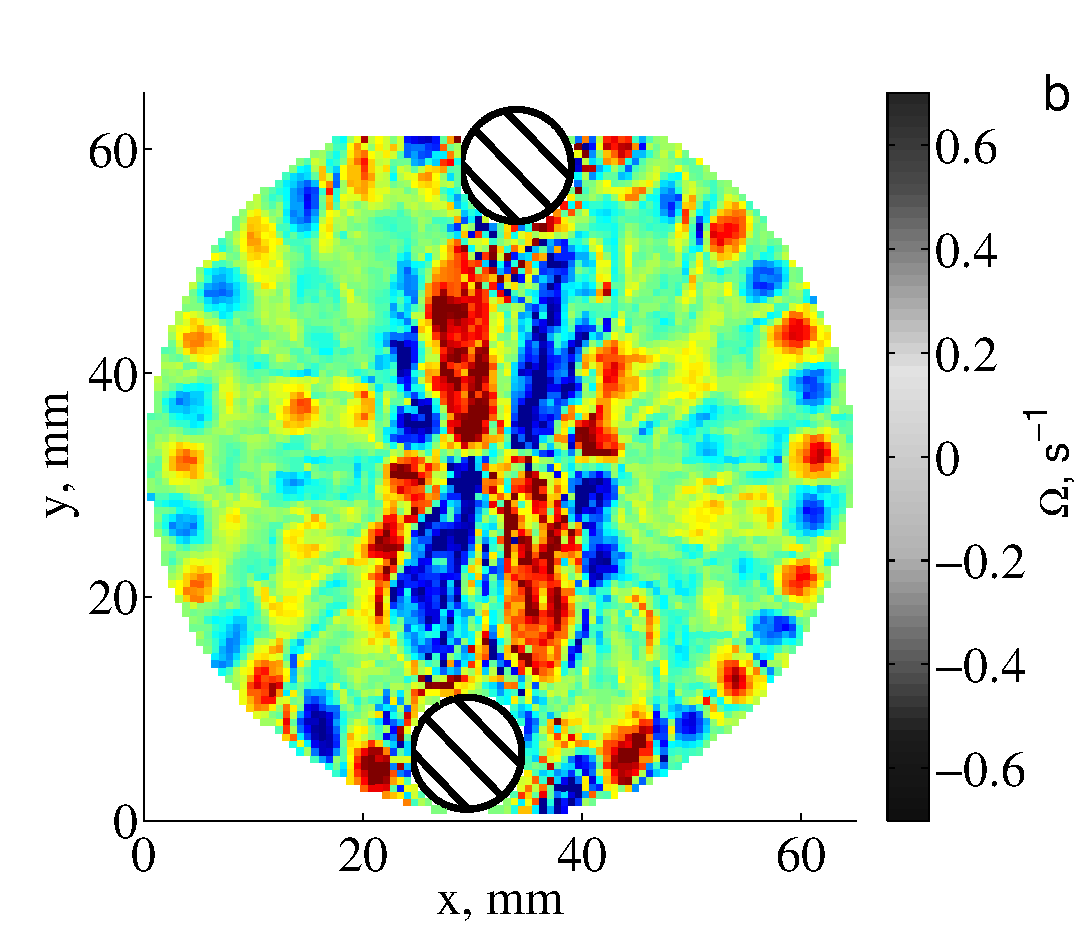
\includegraphics[width=1\linewidth]{article3/pic_06b.eps} \\ б)}
 \end{minipage}
 \caption{Поле завихренности $\Omega$ в цилиндрическом сосуде, в котором установлены два пластиковых столбика. На вставке – завихренность до установки столбиков. Цветовая шкала для завихренности общая.}
 \label{img:vort_st} 
\end{figure}

Для проверки данного предположения симметрия цилиндрического сосуда была нарушена установкой двух пластиковых столбиков диаметром 6.5 мм, размещаемых диаметрально противоположно вблизи стенки сосуда. На рис. \ref{img:vort_st} показано поле завихренности до и после установки столбиков. В сосуде без вставок на поверхности жидкости возбуждается только радиальная волна и вихревого движения не наблюдается. После установки столбиков на поверхности хорошо возбуждаются азимутальные моды и появляется серия вихрей вдоль стенки сосуда аналогично системе вихрей на рис. \ref{img:wave_az}. Поскольку обе моды возбуждаются на одной частоте, их волновые векторы должны быть близки по модулю (в пределах резонансной ширины мод) и иметь разные направления. В квадратном сосуде независимо от частоты накачки угол между волновыми векторами возбужденных волн составляет $90^\circ$. В цилиндрическом сосуде радиальную моду на большом удалении от центра сосуда можно рассматривать как плоскую волну, волновой вектор которой направлен перпендикулярно стенке сосуда. Резонансную моду с малым радиальным числом $n$ и большим азимутальным числом $m$ по аналогии с модами шепчущей галереи для акустических волн можно рассматривать как распространяющуюся вдоль границы сосуда волну. Поэтому мы полагаем, что за формирование вихревого движения здесь отвечает взаимодействие двух поверхностных волн, волновые векторы которых направлены под углом друг к другу.
%\section{Выводы} \label{sect3_3}

Таким образом было экспериментально показано, что стоячие волны на поверхности жидкости в сосуде, который совершает гармонические колебания в вертикальном направлении с амплитудой переменного ускорения ниже порога параметрической неустойчивости, могут генерировать вихревое течение. В квадратном сосуде структура вихревого движения имеет вид квадратной решетки с периодом, равным длине стоячих волн. В цилиндрическом сосуде вихревое движение наблюдается только при возникновении азимутальных мод, которые возможны при амплитудах накачки выше порога параметрической неустойчивости. Искусственное понижение симметрии цилиндрического сосуда, которое разрешает генерацию азимутальных мод при малых амплитудах накачки, позволяет формировать вихревое движение при накачке значительно ниже порога параметрической неустойчивости Фарадея. Исходя из этих наблюдений и принимая во внимание степенную зависимость завихренности от амплитуды волн, можно утверждать, что в сосудах разной симметрии вихревое движение возникает тогда, когда на поверхности жидкости распространяется пара волн с неколлинеарными волновыми векторами.

\section{Нелинейное возбуждение завихренности поверхностными волнами} \label{sect3_4}
Для описания вихревого движения формируемого волновым движение нашими соавторами по работе \cite{F6} из Института Теоретической Физики им.Л.Д. Ландау была построена теоретическая модель генерации вихревого движения нелинейно взаимодействующими волнами, распространяющимися под углом друг к другу. Подробное её описание и вывод можно найти в работах \cite{F6, Parfenyev2016}. Здесь же остановимся на выводах необходимых для интерпретации экспериментальных результатов. Для граничных условий соответствующих двум перпендикулярным стоячим волнам (см. ур-ние \ref{eq:waveStand}), было найдено приближенное распределение вертикальной составляющей завихренности по поверхности жидкости:
\begin{equation}
\label{eq:vortStand}
\Omega = -(1 + \sqrt{2})sin \phi H_1 H_2 \omega k^2 sin(kx)sin(ky).
\end{equation}
Стоит отметить, что полученный результат не зависит от времени. Так же несмотря на то, что вязкость существенна при выводе этого решение, ее нет в конечном результате. Для экспериментального изучения этого эффекта важно обратить внимание на множитель включающий разницу фаз между стоячими волнами в разных направлениях. В квадратной ячейке, разница фаз волн, возбуждаемых вертикальной тряской будет равно нулю. Поэтому для экспериментального изучения полученной теоретической модели использовалась прямоугольная ячейка размерами 49 на 50 мм$^2$. Ненулевая разница фаз будет возникать за счет различия резонансных условиях в двух перпендикулярных направлениях.
\begin{figure}[ht] 
 \center
 \includegraphics [scale=1.5] {article4/pic_01.jpg}
 \caption{Экспериментальная установка для регистрации вихревых движений на поверхности воды. а) Схема установки: 1 - ячейка, 2 - вода, 3 - виброплатформа, 4 - фотоаппарат, 5 - фотовспышка. b) Вогнутый или выпуклый мениск формируется на краю стенок в зависимости от количества воды, используемой для заполнения сосуда. с) Конфигурация водяного мениска в квадратной ячейке, имеющей стенки разной высоты, предназначенная для подавления генерации волн от пары соседних стенок. Стрелки показывают направление распространения волны.} 
 
 \label{img:setup50} 
\end{figure}
Для проверки теоретических предсказаний использовались две ячейки различной геометрии, показанные на рис. \ref{img:setup50}. В ячейке размерами 49 на 50 мм (рис. \ref{img:setup50} б) стенки имеют одинаковую высоту, поэтому на поверхности жидкости устанавливаются стоячие волны. В то время как у ячейки, показанной на рис. \ref{img:setup50} с противоположные стенки имеют разную высоту. Форма мениска у противоположных стенок будет так же отличаться. Меняя уровень воды можно добиться того, что на поверхности воды будут возбуждаться бегущие волн вместо стоячих.
Стационарная картина стоячих капиллярных волн формируется в течении 1-2 с после включения возбуждения. Одновременно с рябью возникает квадратная решетка вихрей на поверхности. Вся картина остается стабильной по крайней мере в течение нескольких минут. Результаты эксперимента представлены на рис. \ref{img:vort_chess} и \ref{img:vort_roll}, где показана завихренность $\Omega$ усредненная по времени. Красный цвет соответствует положительной завихренности, синий цвет - отрицательной завихренности, цветовая шкала, определяющая значение завихренности, так же представлена на рисунке справа.

\begin{figure}[ht] 
 \center
 \includegraphics [scale=.7] {article4/pic_02.eps}
 \caption{Завихренность в ячейке 50 x 49 мм$^2$ при возбуждении поверхностных волн с частотой 42.7 Гц. Наблюдается шахматноподобный паттерн поля завихренности соответствующий теоретическому выражению (14). Периоды решетки в $X$ и $Y$ направлениях равны длине волны.} 
 \label{img:vort_chess} 
\end{figure}

\begin{figure}[ht] 
 \center
 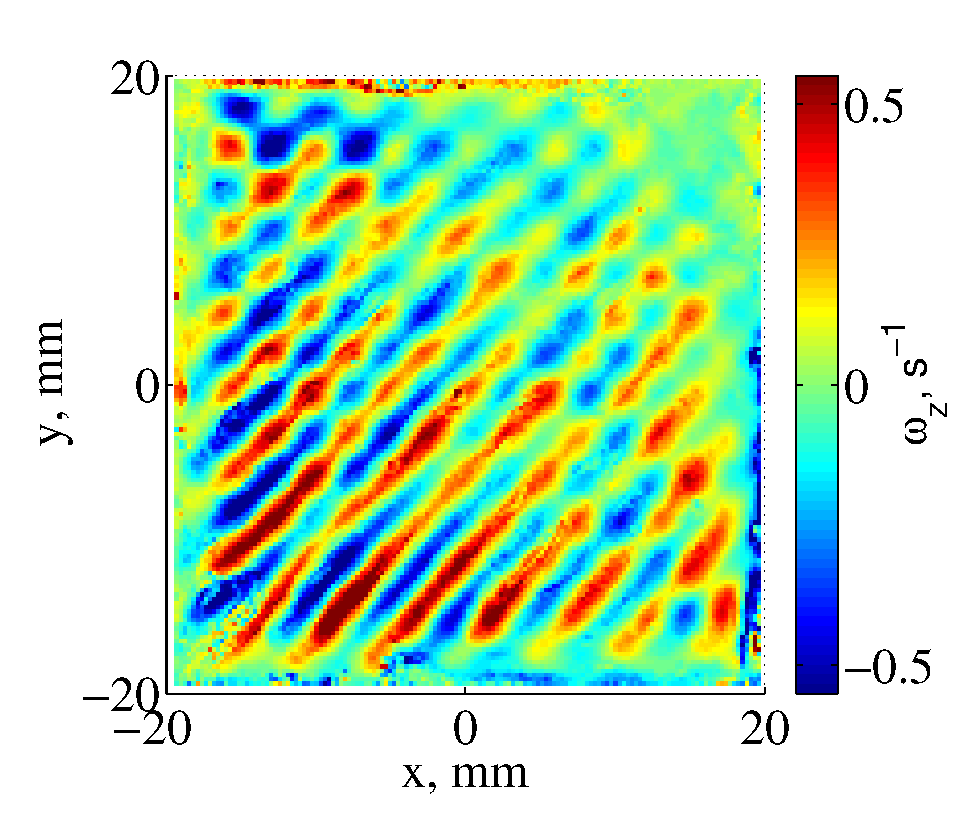
\includegraphics [scale=.7] {article4/pic_03.eps}
 \caption{Завихренность в ячейке 40 х 40 мм $^2$ при возбуждении поверхностных волн с частотой 54 Гц. Две стенки ячейки соответствующие левой и нижней части рисунка немного ниже, чем остальные станки. Уровень воды скорректирован, чтобы в основном возникало две бегущие волны от более низких стенок. Знакопеременные полосы положительной и отрицательной завихренности, направленные параллельно диагонали квадратной ячейки, согласуются с теоретическим выражением (16).} 
 \label{img:vort_roll} 
\end{figure}


Для объяснения результатов сначала заметим, что волны возбуждаются мениском воды, сформированным около стенок. Следовательно, действующие силы локализованы около стен и можно использовать свободные гидродинамические уравнения для описания движения воды не очень близко к стенам. Мы имеем дело с почти линейными волнами заданной частоты, амплитуда волн определяется пристенными силами и граничными условиями. В ячейке возникают только волны распространяющиеся перпендикулярно от стенок прямоугольной ячейки. Резонансные частоты соответствуют волнам с длиной волны соответствующей граничному условию: длина стенок ячейки равна целому числу длин волн с точностью до некоторой поправки, связанной с пристеночной областью. Линейный размер сосуда достаточен, чтобы расстояние в частотном пространстве между соседними резонансами было больше, чем ширина резонансов. Волны распространяющиеся в других направлениях не возбуждаются, так как мощность передаваемая от мениска волне в этом случае пренебрежимо мала.

На рисунке \ref{img:vort_chess} показана завихренность наблюдаемая в почти квадратной ячейке, где стоячие волны возбуждаются в $X$ и $Y$ направлениях.


Мы также проводили эксперименты с квадратной ячейкой, где разница фаз $\phi \ll 1$ (см. рис. \ref{img:vort_square}). Видно что распределение завихренности на рис. \ref{img:vort_square} и \ref{img:vort_chess} существенно отличаются. Для описания распределения завихренности на поверхности следует учитывать затухание волны вдоль направления распространения волны из-за вязкого затухания. 

Амплитуда завихренности как функция амплитуды волны показана на рисунке \ref{img:vort_ampl}. Высота отклонения поверхности вызванная волнами была измерена лазерным лучом отраженным от жидкой поверхности. Размер лазерной проекции на экран может быть пересчитан в амплитуду наклона поверхности $kH$, где $H$ амплитуда наибольшей волны. График на рисунке \ref{img:vort_ampl} показывает квадратичную зависимость завихренности от угловой амплитуды волны, что соответствует нашим теоретическим предсказаниям.

\begin{figure}[ht] 
 \center
 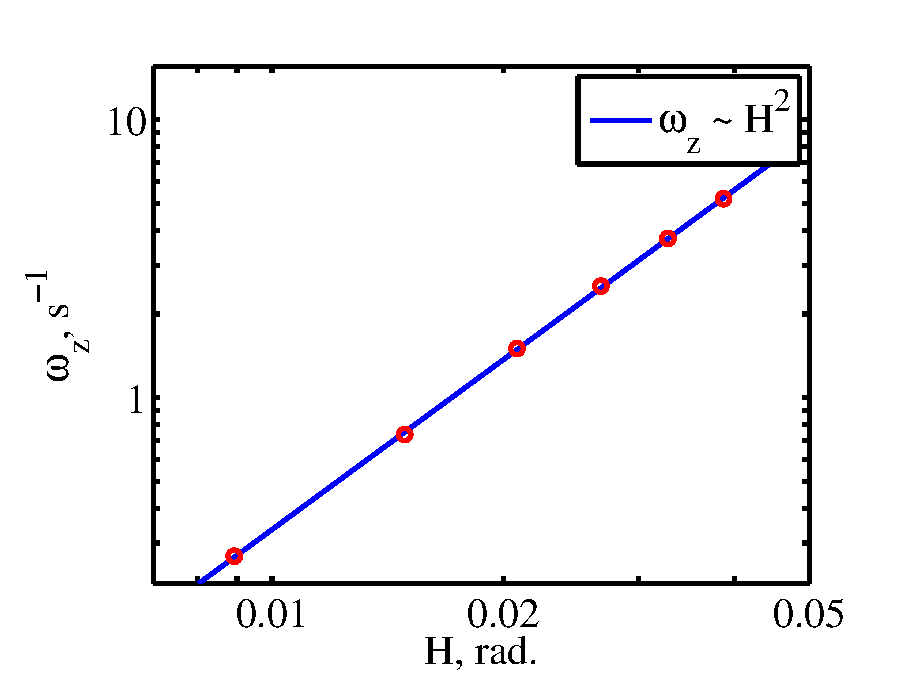
\includegraphics [scale=.7] {article4/pic_04.eps}
 \caption{Амплитуда завихренности для различных амплитуд накачки в ячейке 50 x 49 мм$^2$, где возбуждаются поверхностные волны с частотой 42.7 Гц, строится в зависимости от амплитуды наклона $kH$. Линия соответствует зависимости $\Omega \sim kH^2$.} 
 \label{img:vort_ampl} 
\end{figure}

На рисунке \ref{img:vort_roll} представлены результат другого эксперимента. В этом эксперименте квадратная ячейка имела стенки разной высоты: две смежные стенки немного ниже, чем две противоположные стенки (см. рис. \ref{img:setup50}). Для устранения мениска ячейка была наполнена водой точно по край высоких стенок. На низких стенках вода образует выпуклый мениск(см рис \ref{img:setup50}с). Таким образом возбуждающие силы приложены исключительно на низких стенках. Пренебрегая эффектом отраженных волн, можно получить грубую модель распространяющихся от низких стенок волн. Тогда отклонение поверхности будет задано как:

\begin{equation}
 \label{eq:vortRun}
h = H_1 cos(\omega t - kx) + H_2 cos(\omega t - ky),
\end{equation}

А уравнение описывающее поле завихренности согласно построенной теоретической модели выглядит как:

\begin{equation}
 \label{eq:OmegaRun}
\Omega = -(1 + \sqrt{2})sin \phi H_1 H_2 \omega k^2 sin(kx-ky).
\end{equation}
Заметим, что результат так же не зависит от времени. Рисунок \ref{img:vort_roll} показывает, что пространственное затухание волн сказывается на распределении завихренности. Учет затухания корректирует выражение (\ref{eq:OmegaRun}), что приводит к разумному качественному согласию между экспериментальными данными и теоретическими предсказаниями.% [7]. 

\section{Выводы}
Открыт новый механизм генерации поверхностной завихренности связанный с взаимодействием нелинейных поверхностных волн в тонком вязким подслоем. 
Экспериментально наблюдена квадратичная зависимость модуля завихренности от угловой амплитуды волны.
Наблюденные экспериментальные распределения вихревого движения, генерируемого взаимно перпендикулярными как стоячими, так и бегущими волнами, качественно хорошо согласуются с теоретической моделью.

Увеличивая амплитуду вертикальных колебаний ячейки можно достичь порога неустойчивости Фарадея. Значительно выше порога, поверхностные волны весьма интенсивны, что приводит к интенсивным вихревым движениям поверхности жидкости, для которых угловая амплитуда приближается к 1. Тогда взаимодействие вихревых движений друг с другом становится значительным \cite{Punzmann}, что приводит, в частности, к образованию каскада энергии \cite{Francois2013}. Результаты наших теоретических и экспериментальных исследований позволяют лучше понять это явление и разработать количественную основу для него.

\clearpage           % Глава 4
\chapter{Генерация вихревого движения гравитационными волнами} \label{chapt4}
%abstract
В предыдущей главе было показано, что капиллярные волны распространяющиеся под углом друг к другу генерируют вихревое движение на поверхности жидкости, так же были показаны и экспериментально подтверждены результаты теоретического исследования системы капиллярных перпендикулярных волн. Стоит заметить, что теоретические построения, объясняющие появление шахматноподобного паттерна вихревого поля, пригодны как для капиллярных, так и для гравитационных волн. В этой главе показаны экспериментальные доказательства применимость построенной теории к гравитационным волнам. Так же обнаружена передача энергии вихревого движения из области накачки в большие масштабы.
%Экспериментально исследована генерация вихревого движения на поверхности воды гравитационными волнами на частотах 3 и 4Гц с длиной волны 17 и 9.7 см, соответственно. Показано, что полученные результаты можно описать в рамках модели формирования завихренности нелинейными волнами. Впервые показано, что амплитуда завихренности на поверхности воды зависит от разности фаз между волнами, распространяющимися под углом 90◦ друг к другу с периодом равным, 360◦. Наблюдена квадратичная зависимость амплитуды завихренности на поверхности от угловой амплитуды волн. Обнаружена передача энергии вихревого движения из области накачки в большие масштабы.

\section{Экспериментальная методика} \label{sect4_2}
На рисунке \ref{img:setup} показана схема установки, предназначенной для изучения вихревых и волновых движений на поверхности воды в диапазоне длин волн от 0.25 до 20 см. Ванна изготовлена из оргстекла толщиной 10 мм. Длина ванны равна 140 см, ширина – 70 см, высота – 40 см. Ребра ванны и верхние борта усилены металлическими уголками для придания конструкции жесткости во избежание развития низкочастотных колебаний при работе волнопродукторов. Ванна разделена съемной перегородкой пополам. В данных экспериментах использовалась половина ванны размерами
70 $\times$ 70 см$^2$. Сверху ванна закрывается прозрачным стеклом во избежание попадания на поверхность воды пыли из воздуха. 

\begin{figure}[ht] 
  \center
  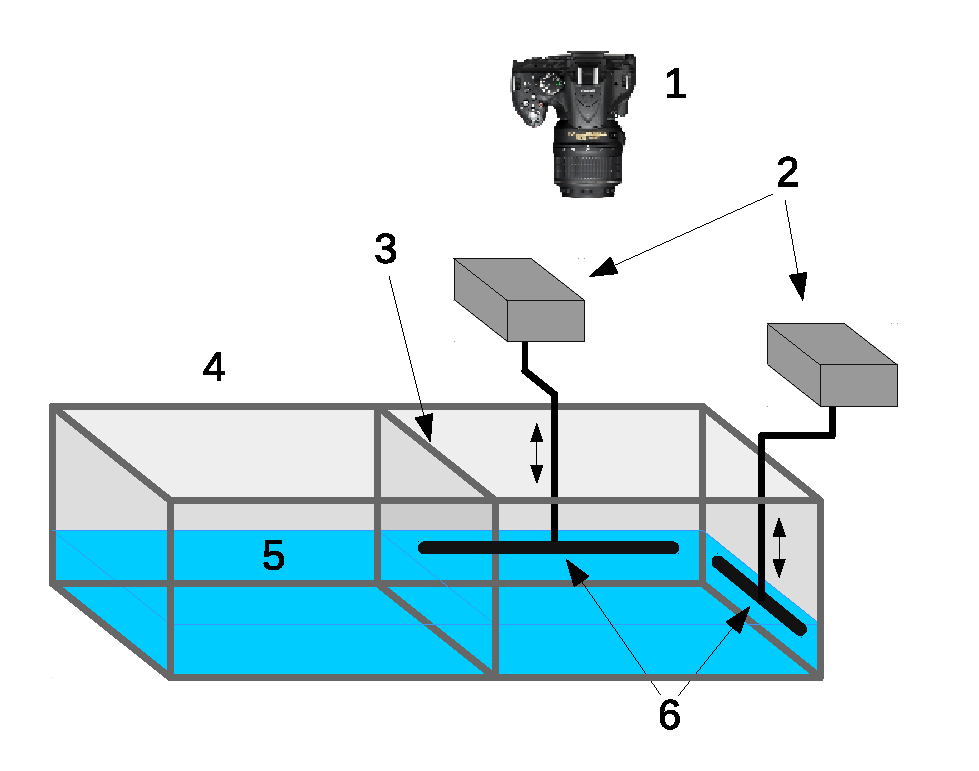
\includegraphics [scale=0.5] {article5/pic_01.eps}
  \caption{Схема установки: 1 – фотоаппарат, 2 – приводы плунжеров, 3 – перегородка, 4 – ванна, 5 – вода, 6 – плунжеры.} 
  \label{img:setup}  
\end{figure}

Ванна установлена на виброизолирующем столе Standa с пневматической подвеской. В ванну, как правило, заливается около 70 л очищенной дистиллированной воды. Глубина воды в ванне составляет около 10 см. Волнопродукторы, состоящие из привода 2 и плунжера 6, монтируются на рамную конструкцию и устанавливаются на столе Standa. Волны на поверхности воды возбуждаются плунжером – трубка из нержавеющей стали диаметром 10 мм, полупогруженной в воду и совершающей вертикальные колебания. Длина трубки равняется 68 см. Расстояние от трубки до стенки ванны равно 1 см. В качестве привода волнопродукторов применяются сабвуферы TS-W254R фирмы Pioneer номинальной мощностью 250 Вт. Синусоидальные сигналы задаются двухканальным генератором Agilemt 33522B, усиливаются и подаются на сабвуферы. В эксперименте разность фаз $\psi$ сигналов в каналах контролируется. Амплитуда волн, распространяющихся от плунжеров, измеряется в центре ванны с помощью лазерного луча отражающегося от поверхности. Для визуализации движения жидкости на поверхность воды насыпается порошок полиамида белого цвета со средним диаметром гранул около 30 мкм. Плотность частиц немного меньше плотности воды, так что они находятся в погруженном состоянии. Поэтому полагаем, что частицы полностью увлекаются потоками жидкости. Гранулы на поверхности слипаются в более крупные образования с размерами порядка 1 мм. Их удается разбить на более мелкие интенсивным возбуждением поверхности. Частички на поверхности подсвечиваются светодиодами, расположенными по периметру ванны. Видеозапись колеблющейся поверхности производится фотоаппаратом Canon EOS 70D в течение 60 с с частотой 24 кадра/c. Такая частота съемки позволяет выбрать снимки колеблющейся поверхности, находящейся в одной фазе волны. Например, при частоте возбуждающей силы, равной 3 Гц во временном отрезке длительностью 10 с получается 30 последовательных снимков, когда волны возбуждения на поверхности имеют одинаковые фазы. Такой отбор снимков позволяет исключить из дальнейшей обработки осциллирующую составляющую перемещения пробной частицы, плавающей на поверхности. Для выявления треков движения частиц на поверхности снимки суммируются.

Обработка полученных исходных снимков программой PIVLab \cite{piv} позволяет вычислить скорости движения частиц $V_x$ и $V_y$, а затем рассчитать завихренность на поверхности по формуле (\ref{eq:defVort}). Распределение энергии по модулю волновых векторов вычисляется усреднением энергии по кольцу в пространстве по формуле:
\begin{equation}
E(k) = \frac{1}{ 2 S \Delta k}\int \frac{d^2 q}{(2 \pi)^2} \lfloor |V_k|^2 \rfloor,
\end{equation}
где интегрирование производится по кольцу от ${k}$ до ${k} + \Delta{k}$. Полученное значение нормируется на площадь поверхности жидкости S. Здесь $V_k$ - Фурье компонента скорости жидкости. Скобки $\lfloor \, \rfloor$ означают усреднение по снимкам, сделанным в разные моменты времени.
	
Групповая скорость волны на частоте 3\,Гц равняется 25\,см/с. Поэтому после включения накачки до возникновения стоячей волны на поверхности воды бегущая волна проходит удвоенное расстояние плунжер-стенка равное 136\,см за 5.5\,с. В представленных ниже результатах мы производили вычисления распределения завихренности и распределения энергии по данным, полученным спустя 15 секунд после включения накачки в интервале длительностью в 5 секунд, чтобы быть уверенным, что амплитуды стоячих волн и завихренность достигли стационарного состояния. Как показывает наши измерения, на временах больше 30 секунд после включения накачки модуль завихренности начинает незначительно уменьшаться. 



\section{Экспериментальные результаты} \label{sect4_3}
На рис. \ref{img:vort_3Hz}а показаны треки полиамидных частиц при накачке поверхности воды на частоте 3\,Гц. При умеренных амплитудах накачки на поверхности хорошо видна решетка из вертикальных и горизонтальных рядов вихрей, аналогичная приведенной в работе \cite{kameke}. Скорость движения полиамидных частиц составляет в среднем 0.02\,см/с. На рис. \ref{img:vort_3Hz}a показана картина, усредненная по времени в интервале 10 секунд, начиная с 15 секунды после включения накачки.


На рис. \ref{img:vort_3Hz}б показано распределение завихренности, полученное обработкой последовательных изображений программой PIVLab. Хорошо видно, что сформированная в ванне решетка, состоит из малых вихрей близкого размера и с противоположными завихренностями. Периоды решетки в X и Y направлениях составляют 17\,см и равняются длине стоячей волны, которая возникла при накачке на частоте 3\,Гц. Суммарная завихренность на поверхности ванны равняется нулю. 

\begin{figure}[ht]
  \begin{minipage}[ht]{0.49\linewidth}
    \center{\includegraphics[width=.82\linewidth]{article5/pic_02a.eps} \\ а)}
  \end{minipage}
  \hfill
  \begin{minipage}[ht]{0.49\linewidth}
    \center{\includegraphics[width=1\linewidth]{article5/pic_02b.eps} \\ б)}
  \end{minipage}
  \caption{a) Треки полиамидных частиц на поверхности воды при накачке двумя плунжерами на частоте 3\,Гц с угловой амплитудой волны в центре ванны $\mu = 0.035$ рад. Плунжеры расположены внизу рисунка и справа. b) Распределение завихренности на поверхности воды при накачке двумя плунжерами на частоте 3\,Гц. Разность фаз $\psi = 90^\circ$.}
  \label{img:vort_3Hz}  
\end{figure}


С повышением уровня накачки амплитуда завихренности каждого вихря на поверхности воды возрастает. На рис.3a показана зависимость корня квадратного из усредненной амплитуды вихрей $\sqrt{\Omega_0}$ на поверхности воды от угловой амплитуды стоячей волны, измеренной в центре ванны. Разность фаз сигналов, подаваемых на плунжеры, $\psi$ равняется $90^\circ$. Хорошо видно, что амплитуда завихренности растет с повышением амплитуды волн по квадратичному закону в соответствии с формулой (\ref{eq:vortStand}). 

На рис. \ref{img:ampl_phase}б показана зависимость амплитуды завихренности на поверхности воды от разности фаз $\psi$ гармонических сигналов, подаваемых на плунжеры на частоте 3\,Гц. Видно, что экспериментальные точки в интервале углов от $0^\circ$ до $180^\circ$ хорошо описываются зависимостью пропорциональной $sin(\psi)$. При изменении разности фаз $\psi$ с $90^\circ$ на $-90^\circ$ амплитуда завихренности сохраняется, но изменяются направления завихренности вихрей в решетке на противоположные. Таким образом, период зависимости $\Omega (\psi)$ равняется $360^\circ$. 

\begin{figure}[ht]
  \begin{minipage}[ht]{0.49\linewidth}
    \center{\includegraphics[width=1\linewidth]{article5/pic_03a.eps} \\ а)}
  \end{minipage}
  \hfill
  \begin{minipage}[ht]{0.49\linewidth}
    \center{\includegraphics[width=1\linewidth]{article5/pic_03b.eps} \\ б)}
  \end{minipage}
  \caption{a) Зависимость корня квадратного амплитуды завихренности $\sqrt{\Omega_0}$ на поверхности воды от угловой амплитуды волн $\mu$ при накачке двумя плунжерами на частоте 3\,Гц. Разность фаз $\psi=90^\circ$ . b) Зависимость амплитуды завихренности $\Omega_0$ от разности фаз между синусоидальными сигналами, подаваемыми на волнопродукторы. Точки – эксперимент, сплошная кривая $\Omega_0 = \,0.183\, sin(\psi)$}
  \label{img:ampl_phase}  
\end{figure}


При высоком уровне накачки картина треков усложняется: сразу после включения на поверхности формируется решетка вихрей, а затем через время порядка минуты на поверхности развиваются структуры с размерами, превосходящими длину волны накачки. Траектории частиц (треки) со временем медленно изменяются, вихри "дышат". 

На рис. \ref{img:ampl_phase}а приведены треки полиамидных частиц на поверхности воды при накачке двумя плунжерами на частоте 4\,Гц, полученные усреднением в течение 15 секунд через 3 минуты после включения накачки. Амплитуда волн, измеренная на расстоянии 3\,см от плунжеров, равняется $1.0\pm0.2$\,мм. На рисунке хорошо видны два сформировавшихся вихря с характерными размерами близкими к 70\,см (длина стороны ванны), а также вихри меньших размеров. Разность фаз при измерении составляла $\psi$ = $120^\circ$. 

На рис. \ref{img:ampl_phase}б показана вихревая структура, генерируемая стоячими волнами с частотой равной 4\,Гц. Вдоль сторон ванны укладывается по семь длин волн, т.е. длина волны на частоте накачки равна 9.7\,см. Хорошо видна решетка вихрей, немного искажаемая двумя большими вихрями, в нижней и верхней частях рисунка. Суммарная завихренность равна нулю. На рис.5 представлена зависимость модуля полной завихренности $|\Omega|$ на поверхности воды, возбуждаемой двумя плунжерами на частоте 4\,Гц, от фазы $\psi$ между колебаниями плунжеров. 

\begin{figure}[ht]
  \begin{minipage}[ht]{0.49\linewidth}
    \center{\includegraphics[width=.85\linewidth]{article5/pic_04a.eps} \\ а)}
  \end{minipage}
  \hfill
  \begin{minipage}[ht]{0.49\linewidth}
    \center{\includegraphics[width=1\linewidth]{article5/pic_04b.eps} \\ б)}
  \end{minipage}
  \caption{a) Треки полиамидных частиц на поверхности воды при накачке двумя плунжерами на частоте 4\,Гц. Амплитуда волн на расстоянии 3\,см от плунжеров равна $H = 1.0 \pm 0.2$\,мм. Плунжеры расположены внизу рисунка и справа. b) Распределение завихренности на поверхности воды. Разность фаз $\psi=120^\circ$.}
  \label{img:vort_4Hz}  
\end{figure}

Начальная разность фаз между колебаниями плунжеров равняется $-30^\circ$. Максимум модуля завихренности наблюдается при $\psi = 120^\circ$ , а минимум – при $\psi = 30^\circ$. Кроме того, очевидно, что в зависимости $|\Omega(\psi)|$ имеется постоянная составляющая, близкая к 0.08\,с$^{-1}$.

Как видно из рис. \ref{img:vort_4Hz} при интенсивной и длительной накачке кроме решетки малых вихрей на поверхности воды возникают вихри больших размеров. Это означает, что в k-пространстве завихренность $\Omega$ и энергия $E$ распространяются из области накачки $\lambda=9.7$\,см на большие масштабы. 
\begin{figure}[ht] 
  \center
  \includegraphics [scale=0.5] {article5/pic_05.eps}
  \caption{Зависимость модуля завихренности на поверхности воды от разности фаз $\psi$ между колебаниями плунжеров на частоте 4\,Гц. Амплитуда волны на расстоянии 3\,см от плунжеров равна $H = 1.0 \pm 0.2$\,мм.} 
  \label{img:phase_4Hz}  
\end{figure}

Результаты вычислений $E(k)$ для вихревых структур, представленных на рис. \ref{img:vort_3Hz} и \ref{img:vort_4Hz}, приведены на рис. \ref{img:spectra} (кривые 1 и 2). Видно, что зависимость $E(k)$ имеет немонотонный характер. В случае возбуждения поверхности волнами на частоте 3\,Гц наблюдается ярко выраженный пик при значении вектора $k = 0.50$\,см$^{-1}$, соответствующего волновому вектору волны накачки. Кроме того, виден пик при значении вектора $k$ равным 1.12\,см$^{-1}$. По-видимому, этот пик может быть связан с формированием завихренности в результате взаимодействия волны генерируемой на частоте накачки и перпендикулярной волны с волновым вектором 1.06\,см$^{-1}$(длина этой волны втрое короче длины волны накачки). Передача энергии в большие масштабы не наблюдается.
\begin{figure}[ht] 
  \center
  \includegraphics [scale=0.5] {article5/pic_06.eps}
  \caption{Распределение энергии $E(k)$ по волновому вектору при накачке двумя плунжерами на частоте 3\,Гц (кривая 1), 4\,Гц (кривая 2) и 6\,Гц (кривая 3).} 
  \label{img:spectra}  
\end{figure}
Однако в случае накачки на частоте 4\,Гц (рис. \ref{img:spectra}, кривая 2) и формирования на поверхности вихревых структур с размерами больше, чем масштаб накачки, энергия $E(k)$ распределена в интервале волновых векторов от области накачки $k \approx 0.85$\,см$^{-1}$ до больших масштабов $k \approx 0.09$\,см$^{-1}$.

Первый пик, на волновом векторе $k = 0.85$\,см$^{-1}$ находится на масштабе накачки. Эта энергия сосредоточена в малых вихрях, которые формируют решетку. Видно, что с уменьшением $k$ наблюдается рост $E(k)$. Максимум распределения $E(k)$ приходится на волновой вектор близкий к 0.09\,см$^{-1}$, который соответствует размерам больших вихрей, сформировавшихся в ванне. Дополнительно на рис. \ref{img:spectra} кривой 3 представлено распределение $E(k)$ при накачке волнами с меньшей длиной волны  (частота 6 Гц, длина волны 4.9 см). На этом распределении также наблюдаются два экстремума, соответствующие масштабу накачки,  $k = 1.8$\,см$^{-1}$  и максимуму энергии,  $k = 0.1$\,см$^{-1}$. Из сравнения распределений 2 и 3 можно заключить, что  масштаб большого вихря не зависит от длины волны накачки и определяется размерами ванны. В области волновых векторов $k > 2\,$см$^{-1}$ значения $E(k)$ более чем на порядок меньше значений амплитуд в основных пиках. Т.е. прямой каскад практически не сформировался: вся энергия уходит на поддержание больших вихрей, где она диссипирует в силу вязких потерь. 

\section{Обсуждение экспериментальных результатов} \label{sect4_4}
Так же как в [F5, F6] в настоящей работе наблюдается решетка из вихрей с периодом равным длине волны накачки. Это свидетельствует о справедливости модели генерации вихрей нелинейными волнами и подтверждает обоснованность применения формул (\ref{eq:vortStand}) и (\ref{eq:vortRun}) для описания завихренности на поверхности жидкости в широком диапазоне длин волн: от 0.5\,см до 17\,см. Следует отметить, что при накачке на частоте 3\,Гц решетка вихрей (рис. \ref{img:vort_3Hz}) является столь же совершенной, как и при накачке капиллярными волнами [F6], где измерения проводились в специальном боксе с чистой атмосферой. В случае гравитационных волн, если ванну не закрывать сверху прозрачным стеклом, то на поверхности чистой воды за время порядка 1 часа формируется тонкая несжимаемая пленка, в результате чего затухание волн значительно возрастает \cite{land}, что отражается на распределении завихренности.

На рис. \ref{img:vort_3Hz}б и \ref{img:vort_4Hz}б, где приведены решетки вихрей, затухание волны не является существенным. Амплитуда отраженной от стенки волны незначительно отличается от амплитуды волны идущей навстречу от плунжера. Согласно формулам (\ref{eq:vortStand}) и (\ref{eq:vortRun}) отличия в этих амплитудах не должны отражаться на квадратичной зависимости завихренности от амплитуд волн. 

Фазовая зависимость амплитуды завихренности при возбуждении волн двумя плунжерами на частоте 3\,Гц очень хорошо описывается периодической функцией пропорциональной $sin(\psi)$. Период функции $\Omega (\psi)$ составляет $360^\circ$, как это и следует из зависимости (\ref{eq:vortStand}). 

Несколько более сложная ситуация наблюдается в экспериментах по исследованию зависимости модуля завихренности от разности фаз $\psi$ между двумя перпендикулярными возбуждающими волнами на частоте 4\,Гц. Как сказано выше, на поверхности воды присутствуют как вихри, формирующие решетку, так и вихри большего масштаба, возникшие в силу нелинейного взаимодействия вихрей и волн. Это хорошо видно на рис. \ref{img:vort_4Hz}a, где на поверхности присутствуют как решетка из одиночных вихрей, так и большие вихри. В связи с этим фазовая зависимость завихренности не может описываться формулой (\ref{eq:vortStand}), а должна содержать некоторый член, отражающей присутствие вихрей большего масштаба. Видно, что накачка вихрей не исчезает даже при $\psi=0^\circ$, то есть присутствие крупномасштабных вихревых течений на поверхности усложняет генерацию вихрей нелинейными поверхностными волнами, описываемую простыми зависимостями (\ref{eq:vortStand}) или (\ref{eq:vortRun}). Величина $|\Omega|$ осциллирует около некоторого пьедестала. По результатам проведенных экспериментов нельзя сказать изменяется ли высота этого пьедестала с ростом разности фаз, поэтому в первом приближении полагаем его постоянным. 

Полученный экспериментальный результат качественно не противоречит модели, представленной в [F6]. Как видно из рис. \ref{img:phase_4Hz} зависимость $|\Omega|$ от разности фаз $\psi$ имеет периодический характер с двумя экстремумами. Период равняется $180^\circ$. Таким образом зависимость модуля завихренности $|\Omega|$ от разности фаз можно описать формулой: 

\begin{equation}\label{eq:fit_abs}
|\Omega| = A |sin(\psi+\psi_0)| + \Omega_0
\end{equation}
где $\psi_0$ - начальный сдвиг фаз, $\Omega_0$ – постоянное слагаемое. Из подгонки зависимости (\ref{eq:fit_abs}) к экспериментальным точкам следует что $\psi_0 = -9^\circ$, $\Omega_0$ = 0.077\,с$^{-1}$, A = 0.028\,с$^{-1}$. Отметим, что постоянное слагаемое определяется структурой больших вихрей, возникающих на поверхности и, отличается в разных реализациях эксперимента при одинаковых начальных условиях. 

Отметим, что абсолютные величины модуля завихренности, полученные в экспериментах по измерению зависимостей амплитуды завихренности от амплитуды волн и разности их фаз приблизительно в 4 раза превосходят теоретическую величину, вычисленную по выражению (\ref{eq:vortStand}). Аналогичное расхождение наблюдалось и в случае капиллярных волн в работе [F6]. 

Так же следует отметить, что при накачке на низких частотах, соответствующих гравитационным волнам, всегда через некоторое время после включения накачки наблюдается формирование структуры (вихрей) с характерным размером больше масштаба накачки. Вихрь может занимать почти всю поверхность ванны, за исключением небольших участков, где располагаются ``смазывающие" вихри, которые обеспечивают нулевую суммарную завихренность, либо их может быть несколько. Отметим также, что при работе с капиллярными волнами большие вихри возникали только после превышения порога параметрической неустойчивости \cite{Francois2013}. 

Как следует из зависимостей, представленных на рис. \ref{img:spectra} (кривые 2 и 3), энергия вихревого движения из области накачки передается в область больших масштабов. Очевидно, что энергия от поверхностных волн поступает сначала в систему вихрей, которые выстроены в решетку. Затем в силу нелинейного взаимодействия энергия распространяется на большие масштабы. Видно, что в основном энергия передается в большие вихри, а в сторону малых масштабов не идет: прямой каскад в сторону больших $k$ (малых масштабов) практически отсутствует.

Обратный каскад наблюдали ранее в экспериментах при генерации фарадеевских волн на поверхности \cite{Francois2014}. Оказалось, что экспериментальное распределение энергии по волновому вектору можно хорошо описать зависимостью $E(k) \sim k^{-5/3}$. Эта зависимость для обратного каскада энергии была предсказана теоретически Крайчнаном \cite{Kraichnan1967} для тонких двумерных слоев жидкости. В случае прямого каскада $E(k) \sim k^{-3}$ \cite{Kraichnan1967}. В наших экспериментах область накачки и область диссипации не разнесены достаточно далеко в k-пространстве, чтобы сформировался развитый каскад, описываемый степенной функцией $k$.

Подчеркнем, что в наших экспериментах мы имеем дело с трехмерным случаем, так как глубина ванны больше глубины проникновения волн на всех используемых частотах накачки. Однако передача энергии из области накачки в большие масштабы, свойственная двумерному случаю, определенно наблюдается. 

Расхождения по абсолютной величине завихренности с теоретической оценкой и формирование обратного каскада, свойственного двумерным системам, в наших трехмерных экспериментах требуют дополнительных экспериментальных и теоретических исследований.

\section{Выводы} \label{sect4_5}
В данной работе впервые экспериментально показано, что завихренность, формируемая на поверхности воды слабо нелинейными гравитационными волнами, зависит от разности их фаз и хорошо описывается выражениями, полученными в работе [F6]. Амплитуда завихренности на поверхности квадратично зависит от амплитуды волн. Таким образом, модель генерации вихревого движения нелинейными волнами применима для описания завихренности на поверхности жидкости не только для волн капиллярного диапазона с длиной волны около 0.5\,см, но и для гравитационных волн с длинами волн порядка 10\,см. Так же наблюдена передача энергии от слабонелинейного волнового движения в систему вихрей, образующих решетку, с последующей передачей в большие масштабы.


%\section{Генерация вихревого движения гравитационными волнами} \label{sect4_3}

\clearpage           % Глава 5
\chapter*{Заключение}						% Заголовок
\addcontentsline{toc}{chapter}{Заключение}	% Добавляем его в оглавление

%% Согласно ГОСТ Р 7.0.11-2011:
%% 5.3.3 В заключении диссертации излагают итоги выполненного исследования, рекомендации, перспективы дальнейшей разработки темы.
%% 9.2.3 В заключении автореферата диссертации излагают итоги данного исследования, рекомендации и перспективы дальнейшей разработки темы.
%% Поэтому имеет смысл сделать эту часть общей и загрузить из одного файла в автореферат и в диссертацию:
В диссертационной работе выполнены экспериментальные исследования капиллярной волновой турбулентности на поверхности жидкого водорода и воды. Выполнено исследование генерации вихревого движение на свободной поверхности жидкости волнами движущимися под углом друг к другу.

1. Впервые наблюден переход от степенного распеределения энергии в инерционном интервале спектра Колмогорова-Захарова к “квазипланковскому” распределению $\omega^{-s}e^{-\omega/\omega_d}$ в области диссипации для капиллярной турбулентности. Экспоненциальная зависимость энергии от частоты в области диссипации $\omega/\omega_d \gg 1$ соответствует теоретическому ожиданию и качественно соответствует численным вычислениям \cite{Ryzhenkova1990}. Граница вязкого затухания $\omega_d$ растет с увеличением амплитуды накачки и зависит от средней высоты волны $\eta_0$ на частоте накачки как $\omega_d \sim \eta^{0.85 \pm 0.05}$. Однако наблюденная зависимость отличается от ожидаемой, показатель степени почти в три раза больше, чем предсказанное значение.

2. Экспериментально показано, что при возбуждении турбулентного состояния на поверхности воды монохроматической или широкополосной накачкой частота высокочастотного края инерционного интервала и характерная частота экспоненциального затухания энергии в диссипативной области отличаются в несколько раз друг от друга и качественно одинаково повышаются с ростом амплитуды накачки по степенному закону с показателем степени, близким к теоретически оцененному значению для случая монохроматического возбуждения. В случае возбуждения широкополосной накачкой наблюдается значительное расхождение между экспериментальными и теоретически оцененными значениями показателя $\beta$.

3. Открыт новый механизм генерации вихревого движения поверхностными волнами распространяющимися под углом друг к другу. Показано, что генерация вихревого движения на поверхности жидкости не является специфической чертой неустойчивости Фарадея.

4. Экспериментально подтверждена теоретическая модель генерации вихревого движения перпендикулярными волнами на поверхности жидкости как для капиллярных, так и для гравитационных волн. Экспериментально подтверждены амплитудная и фазовая зависимости завихренности: амплитуда завихренности на поверхности воды квадратично зависит от амплитуды волн, и зависит как $sin(\psi)$ от разности фаз $\psi$ между стоячими волнами в перпендикулярных направлениях. 

%5. Экспериментально наблюдена передача энергии от системы вихрей, образующих решетку, в большие вихревые масштабы.
%Экспериментально показано, что стоячие волны на поверхности жидкости в сосуде, который совершает гармонические колебания в вертикальном направлении с амплитудой переменного ускорения ниже порога параметрической неустойчивости, могут генерировать вихревое течение. В квадратном сосуде структура вихревого движения имеет вид квадратной решетки с периодом, равным длине стоячих волн. В цилиндрическом сосуде вихревое движение наблюдается только при возникновении азимутальных мод, которые возможны при амплитудах накачки выше порога рога параметрической неустойчивости. Искусственное понижение симметрии цилиндрического сосуда, которое разрешает генерацию азимутальных мод при малых амплитудах накачки, позволяет формировать вихревое движение при накачке значительно ниже порога параметрической неустойчивости Фарадея. Исходя из этих наблюдений и принимая во внимание степенную зависимость завихренности от амплитуды волн, можно утверждать, что в сосудах разной симметрии вихревое движение возникает тогда, когда на поверхности жидкости распространяется пара волн с неколлинеарными волновыми векторами.
% В частности этот механизм приводит к перемешиванию поверхности, которое может быть характерезовано как диффуззионным коэффициентом $D$ соответсующиего четвертому порядку волновой амплитуды, так из прямым действием волн на поверхности жидкости \cite{Falkovich, Buhler}. Данная задача требует дальнейшего исследования. Несмотря на то, что эксперименты производились в капиллярной области, наши теоретические построения также применимы и в на гравитационной области. Для примера соответствующая теория может быть использована для анализа вихревого движения на поверхности океана.

%Основные результаты работы заключаются в следующем.
%\input{common/concl}
%И какая-нибудь заключающая фраза.
%
%Последний параграф может включать благодарности.  В заключение автор
%выражает благодарность и большую признательность научному руководителю
%Иванову~И.И. за поддержку, помощь, обсуждение результатов и научное
%руководство. Также автор благодарит Сидорова~А.А. и Петрова~Б.Б. за
%помощь в работе с образцами, Рабиновича~В.В. за предоставленные
%образцы и обсуждение результатов, Занудятину~Г.Г. и авторов шаблона
%*Russian-Phd-LaTeX-Dissertation-Template* за помощь в оформлении
%диссертации. Автор также благодарит много разных людей и
%всех, кто сделал настоящую работу автора возможной.
      % Заключение
%\include{Dissertation/acronyms}        % Список сокращений и условных обозначений
%\include{Dissertation/dictionary}      % Словарь терминов
\clearpage                                  % В том числе гарантирует, что список литературы в оглавлении будет с правильным номером страницы
%\hypersetup{ urlcolor=black }               % Ссылки делаем чёрными
%\providecommand*{\BibDash}{}                % В стилях ugost2008 отключаем использование тире как разделителя 
\urlstyle{rm}                               % ссылки URL обычным шрифтом
\ifdefmacro{\microtypesetup}{\microtypesetup{protrusion=false}}{} % не рекомендуется применять пакет микротипографики к автоматически генерируемому списку литературы
%\insertbibliofull                           % Подключаем Bib-базы
\ifdefmacro{\microtypesetup}{\microtypesetup{protrusion=true}}{}
\urlstyle{tt}                               % возвращаем установки шрифта ссылок URL
%\hypersetup{ urlcolor={urlcolor} }          % Восстанавливаем цвет ссылок
%(pam-pam \cite{Brazhnikov_bound} taram)

%\chapter*{Публикации по теме диссертации}						% Заголовок
\addcontentsline{toc}{chapter}{Публикации по теме диссертации}	% Добавляем его в оглавление


[F1] Brazhnikov M.Yu., Abdurakhimov L.V., Filatov S.V., Levchenko A.A., "Quasi-Planck" scpectra of capillary turbulence on the surface of liquid hydrogen // JETP Lett. 2011.V. 93. P. 34.

[F2] Л.В. Абдурахимов, М.Ю. Бражников, А.А. Левченко, И.А. Ремизов, С.В. Филатов, "Турбулентный капиллярный каскад вблизи края инерционного интервала на поверхности квантовой жидкости", Письма в ЖЭТФ, том 95 вып. 12, с. 751-760 (2012)

[F3] Л.В. Абдурахимов, М.Ю. Бражников, А.А. Левченко, И.А. Ремизов, С.В. Филатов, "Кинетическая и дискретная турбулентность на поверхности квантовой жидкости", УФН, том 182, 8, с. 879 (2012)

[F4] С.В. Филатов, М.Ю. Бражников, А.А. Левченко, "Метод пространственной регистрации волн на поверхности прозрачной жидкости", ПТЭ, 1, с. 107-112, (2014)

[F5] С.В. Филатов, М.Ю. Бражников, А.А. Левченко, "Формирование вихревого течения волнами на поверхности жидкости", Письма в ЖЭТФ, том 102, вып. 7, с. 486-490 (2015)

[F6] S.V. Filatov, V.M. Parfenyev, S.S. Vergeles, M.Yu. Brazhnikov, A.A. Levchenko, V.V. Lebedev, "Nonlinear Generation of Vorticity by Surface Waves", Physical Review Letters, 116, 054501 (2016)

[F7]. С.В. Филатов, М.Ю. Бражников, А.А. Левченко,  А.М. Лихтер, "Турбулентность в системе капиллярных волн на поверхности воды", Поверхность, 10, с. 69-76 (2016)

[F8] С.В. Филатов, С.А. Алиев, А.А. Левченко, Д.А. Храмов, "Генерация вихрей гравитационными волнами на поверхности воды", Письма в ЖЭТФ, том 104, вып.  10, с. 714-720 (2016)


\begin{thebibliography}{99}

\bibitem{zakh}
V.E. Zakharov, V.S. L'vov, G. Falkovich, Kolmogorov Spectra of Turbulence I, Springer-Verlag, (1992).

\bibitem{2}
М.Ю. Бражников, Г.В. Колмаков, А.А. Левченко, Л.П. Межов-Деглин, Капиллярная турбулентность на поверхности жидкого водорода, Письма в ЖЭТФ, том 73, вып 8, стр 443-446 (2001).
 
\bibitem{3}
G.V. Kolmakov, A.A. Levchenko, M.Yu. Brazhnikov et al, Phys. Rev. Lett. 93, 074501 (2004).

\bibitem{4}
V.E. Zakharov, N.N. Filonenko, J. App. Mech. Tech. Phys. 8, 62, (1967)

\bibitem(5)
V.M. Malkin, JEPT 86, 1263 (1984).

\bibitem{6}
I.V. Ryzhenkova, G.E. Falkovich, JEPT 98, 1931 (1990).

\bibitem{Brazhnikov_IET}
A.A. Levchenko, M.Yu. Brazhnikov, L.P. Mezhov-Deglin. Excitation and Detection of Nonlinear Waves on a Charged Surface of Liquid Hydrogen. IET, 45(6), 758–763 (2002).

\bibitem{Brazhnikov_bound_freq}
М.Ю. Бражников, Г.В. Колмаков, А.А. Левченко, Л.П. Межов-Деглин, Изменение граничной частоты инерционного интервала тербулентности капиллярных волн на поверхности жидкого водорода. Письма в ЖЭТФ, 74(12), 660–663 (2001).
%-----------------------------------
\bibitem{9}
1. Zakharov V.E., L’vov V.S., Falkovich G. Kolmogorov Spectra of Turbulence I. Springer–Verlag, 1992.

\bibitem{10}
2. Falcon E., Laroche C., Fauve S. // Phys. Rev. Lett. 2007. V. 98. P. 094503.

\bibitem{11}
3. Henry E., Alstrшm P., Levinsen M.T. // Europhys. Lett. 2000. V. 52 (1). P. 27.

\bibitem{12}
4. Shats M., Punzmann H., Xia H. // Phys. Rev. Lett. 2010. V. 104. P. 104503.

\bibitem{13}
5. Denissenko P., Lukaschuk S., Nazarenko S. // Phys. Rev. Lett. 2007. V. 99. P. 014501.

\bibitem{14}
6. Shats M.G., Xia H., Punzmann H. // Phys. Rev. E. 2005. V. 71. P. 046409.

\bibitem{15}
7. Von Kameke A., Huhn F., Fernandez-Garcia G., Munuzuri A.P., Perez-Munuzuri V. // Phys. Rev. Lett. 2011. V. 107. P. 074502.

\bibitem{16}
8. Филатов С.В., Бражников М.Ю., Левченко А.А. // Письма в ЖЭТФ. 2015. Т. 102. № 7. С. 486.

\bibitem{17}
9. Filatov S.V., Parfenyev V.M., Vergeles S.S., Brazhnikov M.Yu., Levchenko A.A., Lebedev V.V. // Phys. Rev. Lett. 2016. V. 116. P. 054501.

\bibitem{Brazhnikov_liq_hydr}
10. Бражников М.Ю., Колмаков, Г.В., Левченко А.А., Турбулентность капиллярных волн на поверхности жидкого водорода // ЖЭТФ. 2002. V. 122. P. 521.

\bibitem{Ryzhenkova}
11. Ryzhenkova I.V., Falkovich G.E., Effect of dissipation on the structure of a stationary wave turbulence spectrum // JETP. 1990. V. 71. P. 1085.

%\bibitem{20}
%12. Brazhnikov M.Yu., Abdurakhimov L.V., Filatov S.V., Levchenko A.A., "Quasi-Planck" scpectra of capillary turbulence on the surface of liquid hydrogen // JETP Lett. 2011.V. 93. P. 34.

%\bibitem{Abdur_quantum}
%13. Абдурахимов Л.В., Бражников М.Ю., Левченко А.А., Ремизов И.А., Филатов С.В., Турбулентный капиллярный каскад %вблизи края инерционного интервала на поверхности квантовой жидкости // Письма в ЖЭТФ. 2012. Т. 95. С. 751.

\bibitem{22}
14. Kartashova E.A. // Physica D. 1991. V. 54. P. 125.

\bibitem{23}
15. Brazhnikov M.Yu., Levchenko A.A., Mezhov-Deglin L.P., Remizov I.A. // JETP Lett. 2014. V. 100. P. 669.

\bibitem{24}
16. Абдурахимов Л.В., Бражников М.Ю., Левченко А.А., Лихтер А.М., Ремизов И.А. // Физика низких температур. 2015. Т. 41. № 3. С. 215.

%\bibitem{25}
%17. Бражников M.Ю., Левченко А.А., Межов-Деглин Л.П. // Приборы и техника эксперимента. 2002. № 6. С. 31.

\bibitem{Brazhnikov_EPL}
M.Y. Brazhnikov, G.V. Kolmakov, A.A. Levchenko, L.P. Mezhov-Deglin, Observation of capillary turbulence on the water surface in a wide range of frequencies // Europhys. Lett. 58 (4), 510-516 (2002)

%%---------------------------------------------------

\bibitem{27}
1. T.H. Havelock, Phil, Mag. 8, 569 (1929).

\bibitem{28}
2. В.А. Калиниченко, С.В. Нестеров, Н.Л. Никитин, С.Я. Секерж-Зенькович, Изв. АН СССР, ФАО 4, 432 (1982).

\bibitem{29}
3. М.Ю. Бражников, А.А. Левченко, Л.П. Межов- Деглин, Приборы и техника эксперимента 45, 31 (2002) [Instr. Exp. Tech. 45, 758 (2002)].

\bibitem{30}
4. J. Miles and D. Henderson, Annu. Rev. Fluid Mech. 22, 143 (1990).

\bibitem{31}
5. M. Faraday, Phil. Trans. R. Soc. London 121, 299 (1831).

\bibitem{32}
6. R. Ramshankar, D. Berlin, and J.P. Gollub, Phys. Fluids A 2, 1955 (1990).

\bibitem{33}
7. A.vonKameke, F. Huhn, G. Fernandez-Garcia, A.P. Munuzuri, and V. Perez-Munuzuri, Phys. Rev. Lett. 107, 074502 (2011).

\bibitem{34}
8. N. Francois, H. Xia, H. Punzmann, S. Ramsden, and M. Shats, Phys. Rev. X 4, 021021 (2014).

\bibitem{35}
9. R. Kraichnan, Phys. Fluids 10, 1417 (1967).

\bibitem{36}
10. O.N. Mesquita, S. Kane, and J.P. Gollub, Phys. Rev. A 45, 3700 (1992).

\bibitem{37}
11. G.G. Stokes, Trans. Cambridge Phil. Soc. 8, 441 (1847).

%\bibitem{38}
%12. Л.Д. Ландау, Е.М. Лифшиц, Теоретическая физика. Т. 6. Гидродинамика. Физматлит, М. (2003).

\bibitem{PIVlab}
13. W. Thielicke and E. J. Stamhuis, J. Open Res. Soft. 2(1), е30 (2014).

\bibitem{Lukaschuk}
14. S. Lukaschuk, P. Denissenko, and G. Falkovich, Eur. Phys. J. Special Topics 145, 125 (2007).

%\bibitem{41}
%15. V.V. Lebedev, V.M. Parfenyev, and S. Vergeles, to be published.

%%-------------------
\bibitem{42}
[1] H. Lamb, Hydrodynamics, 6th ed. (Cambridge University Press, Cambridge, England, 1975).

\bibitem{43}
[2] L. D. Landau and E. M. Lifshitz, Course of Theoretical Physics, Vol. 6, Fluid Mechanics, 2nd English ed., (Pergamon Press, Oxford, England, 1987).

\bibitem{44}
[3] A. von Kameke, F. Huhn, G. Fernandez-Garcia, A. P. Munuzuri, and V. Perez-Munuzuri, Phys. Rev. Lett. 107, 074502 (2011).

\bibitem{Shats_inverse}
[4] N. Francois,H.Xia, H. Punzmann, and M. Shats, Phys. Rev. Lett. 110, 194501 (2013).

\bibitem{46}
[5] N. Francois, H. Xia, H. Punzmann, S. Ramsden, and M. Shats, Phys. Rev. X 4, 021021 (2014).

\bibitem{47}
[6] M. Faraday, Phil. Trans. R. Soc. London 121, 299 (1831).

\bibitem{48}
[7] See Supplemental Material at http://link.aps.org/
supplemental/10.1103/PhysRevLett.116.054501 for details of the calculations.

\bibitem{49}
[8] W. Thielicke and E. J. Stamhuis, J. Open Res. Software 2, e30 (2014).

\bibitem{Falkovich}
[9] G. Falkovich, J. Fluid Mech. 638, 1 (2009).

\bibitem{Buhler}
[10] O. Bühler and M. Holmes-Cerfon, J. Fluid Mech. 638,5 (2009).

\bibitem{Punzmann}
[11] H. Punzmann, N. Francois, H. Xia, G. Falkovich, and M. Shats, Nat. Phys. 10, 658 (2014).



\bibitem{parf}
S.V. Filatov, V.M. Parfenyev, S.S. Vergeles et al., Phys.Rev. Lett. { 116}. P. 054501 (2016).

\bibitem{kameke}
A. Von Kameke, F. Huhn, G. Fernandez-Garcia et al., Phys. Rev. Lett. { 107}. P. 074502 (2011).

\bibitem{shats}
N. Francois, H. Xia, H. Punzmann et al., Pys.Rev.Lett. { 110 }, 194501 (2013)

\bibitem{fil}
С.В. Филатов, М.Ю. Бражников, А.А. Левченко, Письма в ЖЭТФ. {f 102}. № 7. С. 486 (2015).

\bibitem{land}
Л.Д. Ландау, Е.М. Лифшиц, Теоретическая физика, т. 6, Гидродинамика. М.: Физматлит, (2003).

\bibitem{piv}
W. Thielicke and E.J. Stamhuis Journal of Open Research Software 2(1)p.e30 (2014).

\bibitem{fran}
N. Francois, H. Xia, H. Punzmann et al., Phys. Rev. X. { 4}, 021021 (2014)

\bibitem{krai}
R. H. Kraichnan, Phys. Fluids, {10}, 1417 (1967).


\end{thebibliography}
      % Список литературы
%\include{Dissertation/lists}           % Списки таблиц и изображений (иллюстративный материал)
%\include{Dissertation/appendix}        % Приложения

\end{document}
